% zamienne marginesy (do druku)

% \documentclass[a4paper, 12pt, twoside]{article}

% zwykłe marginesy (na komputer)

\documentclass[a4paper, 12pt]{article}
\usepackage[T1]{fontenc}
\usepackage[utf8]{inputenc}
\usepackage{graphicx} % includegraphics and all images tools
\usepackage{float}
\usepackage[intlimits]{amsmath}
\usepackage{amssymb,amsfonts}
% \usepackage{txfonts} arial 
\usepackage{fancyhdr} % Extensive control of page headers and footers
\usepackage{fancyvrb}
\usepackage{subcaption}
\usepackage{chngcntr}
\usepackage[polish]{babel}
\usepackage{polski}
\usepackage{listings}
\usepackage[hyphens]{url}
\usepackage{placeins}
\usepackage{hyperref} % links and urls in document
\usepackage{indentfirst} % wcięcie pierwszego akapitu
\usepackage{pdfpages} % include pdf in document - title page
\usepackage[figuresleft]{rotating}
\usepackage{afterpage}
\usepackage[bottom]{footmisc}
\usepackage{multirow}
\usepackage{vcell}
\usepackage{diagbox}
\usepackage{geometry}
% \geometry{a4paper, top=25mm, inner=30mm, outer=20mm, bottom=25mm, headheight=125mm}
\usepackage{changepage}

% nagłówki
% \usepackage{fancyhdr}

% podpisy nad tabelami
\floatstyle{plaintop}
\restylefloat{table}
% end

% fbox dookola bialych zdjec
\fboxsep=0mm%padding thickness
\fboxrule=0.5pt%border thickness
%end

\usepackage{makecell}

\usepackage{pifont}
\usepackage{xcolor}
\newcommand{\cmark}{\textcolor{green!80!black}{\ding{51}}}
\newcommand{\xmark}{\textcolor{red}{\ding{55}}}
\newcolumntype{L}{>{\centering\arraybackslash}m{4cm}}
\newcommand\blankpage{%
    \null
    \thispagestyle{empty}%
    \addtocounter{page}{-1}%
    \newpage}
% listingi i spis listingów
\usepackage{listings}
\usepackage{caption}

\DeclareCaptionType{code}[Listing][Spis listingów]
\lstset{language=Python,
    frame=single, % adds a frame around the code
    xleftmargin=3.4pt,
    xrightmargin=3.4pt,
    keywordstyle=\color{black},
    basicstyle=\scriptsize\ttfamily,
    commentstyle=\color{black}\ttfamily,
    rulecolor=\color{black},
    upquote=true,
    numbers=left,
    numberstyle=\tiny\color{gray},
    stepnumber=1,
    numbersep=8pt,
    showstringspaces=false,
    breaklines=true,
    frameround=ftff,
    frame=single,
    belowcaptionskip=0.2em,
    belowskip=0.2em,}

%linki
\hypersetup{
  colorlinks = true, %Colours links instead of ugly boxes
  urlcolor = black, %Colour for external hyperlinks
  linkcolor = black, %Colour of internal links
  citecolor = black %Colour of citations
}

\newcommand{\myparagraph}[1]{\paragraph{#1}\mbox{}\\}

\restylefloat{table}
\let\svaddcontentsline\addcontentsline
\captionsetup{justification=centering} 
\addto\captionspolish{\renewcommand{\figurename}{Rys.}}
\addto\captionspolish{\renewcommand{\tablename}{Tab.}}
\addto\captionspolish{\renewcommand{\contentsname}{Spis treści}}
\addto\captionspolish{\renewcommand{\abstractname}{}}
\addto\captionspolish{\renewcommand{\listfigurename}{Spis rysunków}}
\addto\captionspolish{\renewcommand{\listtablename}{Spis tabel}}
\renewcommand{\baselinestretch}{1.5}
\numberwithin{figure}{section}
\counterwithin{table}{section}
\counterwithin{code}{section}

\begin{document}
\begin{sloppypar}

% nazwa rozdziału w nagłówku:

% \pagestyle{fancy}
% \renewcommand{\sectionmark}[1]{\markboth{#1}{#1}}
% \renewcommand{\headrulewidth}{0pt} % Width of line at top of page
% \fancyhead[R]{\leftmark}
% \fancyhead[L]{}


% Strona tytułowa:


\includepdf{title_page.pdf}
\pagenumbering{arabic}
\setcounter{page}{2}
\setcounter{secnumdepth}{3}

% Spis treści:

\tableofcontents
% \pagebreak

\newpage

% Wstęp

\section{Wstęp}

Fotografia to stosunkowo nowy wynalazek --- nie minęło nawet 200 lat od wykonania pierwszego znanego nam zdjęcia, słynnego ``Widoku z okna w Le Gras'' z~1826 roku \cite{fotografia}. Początki uwieczniania obrazu przez ludzi były jednak diametralnie różne od tego, co znane jest dzisiaj. Do momentu wynalezienia matrycy światłoczułej (czyli powstania fotografii cyfrowej), rozwój technik fotograficznych polegał jedynie na ulepszaniu technologii bazującej na światłoczułości soli srebra \cite{fotografia}. Fotografia wkrótce została rozpowszechniona na całym świecie. Dało jej to ogromne znaczenie historyczne i kulturowe --- zdjęcia mogą być zarówno dziełami sztuki, jak i dokumentacją ważnych wydarzeń. Powstał również zawód fotografa, który przeszedł wiele zmian na przestrzeni czasu --- początkowo były to osoby, do których należało się udać, żeby mieć możliwość uwiecznienia swojego wizerunku. Zmiana charakterystyki wspomnianej profesji zaczęła następować wraz z wynalezieniem fotografii cyfrowej oraz rozwojem technologii informatycznych. W 1957 roku powstał pierwszy obraz cyfrowy, wykonany przez Russella Kirscha, amerykańskiego naukowca-informatyka. Był to skan analogowej fotografii jego 3-miesięcznego syna \cite{firstdigitalphoto}. Dwanaście lat później Willard S. Boyle oraz George E. Smith wynaleźli matrycę CCD\footnote{ang. CCD --- charge-coupled device.}. Z perspektywy czasu okazało się to być na tyle istotnym dokonaniem, że jego autorzy otrzymali w~2009 roku nagrodę Nobla \cite{nobelfoto}. Powstanie i rozpowszechnienie fotografii cyfrowej zbiegło się też z okresem najszybszego wzrostu ogólnej dostępności Internetu. Na przełomie tysiącleci pojawiły się media społecznościowe, w tym niektóre niemal całkowicie oparte na publikowaniu obrazów, na przykład Instagram (\url{www.instagram.com}). Ludzie codziennie dzielą się milionami zdjęć, a~największe konta posiadają nawet kilkaset milionów obserwujących \cite{instagram}. Inne media społecznościowe również w dużej mierze polegają na możliwości udostępniania zdjęć. Wszystko to powoduje, że zawód fotografa jest obecnie zupełnie inny, niż w~czasach przed wynalezieniem aparatu cyfrowego. Pojawiają się nowe rodzaje zleceń --- profesjonalnie wykonane zdjęcia potrzebne są nie tylko po to, aby uwiecznić przełomowe momenty w życiu człowieka lub umieścić je w prasie, ale też stanowią niezwykle ważny środek przekazu w reklamie. 

Powszechna dostępność aparatów cyfrowych oraz rozwój technologii pozwalający na polepszenie stosunku ceny do jakości sprzętu fotograficznego spowodowały jednak, że pojawiło się wielu fotografów, a co za tym idzie --- utworzyła się większa konkurencja na rynku. Trudniej jest znaleźć nowych klientów. Aby pozyskać zlecenia, w obecnych czasach konieczna jest więc odpowiednia promocja świadczonych usług. W 2022 roku kanadyjski magazyn Format przeprowadził ankietę. Brało w niej udział 3 898 fotografów z 97 krajów. Według zebranych odpowiedzi, na najważniejsze źródła pozyskiwania nowych klientów składają się polecenia od poprzednich klientów (61\% respondentów), strona internetowa z portfolio (40\%), Instagram (38\%), Facebook (25\%) oraz wyszukiwania w Google (22\%) \cite{stateofphotography}. Z danych tych wynika, że najbardziej istotnym internetowym narzędziem do pozyskiwania nowych klientów są personalne strony internetowe z portfolio fotografa.

To, jak ma wyglądać portfolio osoby świadczącej usługi fotograficzne, w dużym stopniu zależy od tego, jaką dziedzinę fotografii reprezentuje jego właściciel. Przykładowo, fotograf ślubny oprócz samego portfolio powinien posiadać na swojej stronie internetowej dokładny opis świadczonych usług, a także przydatne informacje pomagające potencjalnemu klientowi podjąć decyzję o kontakcie. Osobie prowadzącej studio fotograficzne przyda się wykaz rekwizytów, a fotografowi produktowemu lista firm, z którymi współpracował. Strona tworzona w ramach pracy inżynierskiej będzie natomiast przeznaczona dla fotografa koncertowego i dziennikarza muzycznego. Przydatnym elementem będzie więc blog, który posłuży do umieszczania relacji z wydarzeń takich, jak koncerty czy festiwale, a także zapewni miejsce do publikowania wypowiedzi w charakterze felietonu lub recenzji.


%% Cel i założenia pracy

\subsection{Cel i założenia pracy}

Celem pracy jest zaprojektowanie oraz implementacja personalnej strony internetowej łączącej cechy strony-wizytówki, blogu z systemem komentowania oraz portfolio fotograficznego. Strona ta ma być miejscem prezentacji osiągnięć fotografa i dziennikarza muzycznego. Etap projektu skupia się na przeglądzie istniejących rozwiązań oraz na wykonaniu projektu graficznego strony. Implementacja polega na stworzeniu dwuczęściowej aplikacji sieciowej przy użyciu systemu zarządzania treścią Strapi oraz szkieletu aplikacyjnego Next.js, umożliwiającego pobieranie danych ze Strapi oraz renderowanie treści po stronie serwera, co pozwala na korzystne pozycjonowanie strony w wyszukiwarkach internetowych. 

%% Układ pracy

\subsection{Układ pracy}

Rozdział pierwszy wprowadza do tematyki oraz problematyki pracy. Drugi rozdział jest przeglądem istniejących rozwiązań --- personalnych stron-wizytówek popularnych zagranicznych fotografów koncertowych, portali społecznościowych używanych w branży, a także blogów i innych stron o tematyce muzycznej. W rozdziale trzecim przedstawione są narzędzia, które zostały wykorzystane podczas projektowania oraz implementacji tworzonej strony internetowej. Rozdział czwarty poświęcony jest projektowi portfolio i~blogu --- znalazły się w nim założenia projektu, wymagania funkcjonalne i~niefunkcjonalne oraz opis realizacji projektu. Piąty rozdział jest prezentacją wykonanej strony internetowej, a szósty podsumowuje realizację projektu, celu oraz założeń pracy.

% Przegląd istniejących rozwiązań 

\newpage

\section{Przegląd istniejących rozwiązań} \label{przeglad}

Fotografia i dziennikarstwo to branże, które wzajemnie od siebie zależą. Zdjęcia urozmaicają relacje prasowe z wydarzeń, powodują, że artykuły są ciekawsze, a~odbiór fotoreportażu jest lepszy wtedy, gdy przedstawiona jest jakaś historia. Aby strona internetowa realizowana na potrzeby tej pracy inżynierskiej była wykonana z zachowaniem najlepszych możliwych praktyk, został przeprowadzony przegląd istniejących rozwiązań posiadających podobne funkcje. Pozwoli to na znalezienie inspiracji, wyciągnięcie wniosków i wykorzystanie ich zarówno podczas projektowania wyglądu strony, jak i na etapie implementacji.

%% Personalne strony-wizytówki fotografów

\subsection{Personalne strony-wizytówki fotografów}

Personalne strony-wizytówki fotografów są zazwyczaj nieskomplikowane pod względem budowy, nawigacji oraz wyglądu. Rozkład elementów powinien być możliwie prosty, żeby potencjalny klient oglądający portfolio mógł skupić się na jego zawartości. W tym podrozdziale zostaną poddane analizie dwie strony profesjonalnych fotografów działających w branży muzycznej.

%%% Ashley Osborn

\subsubsection{Ashley Osborn} \label{ashley}

Ashley Osborn jest amerykańską fotografką zamieszkałą w Los Angeles. Specjalizuje się w dokumentowaniu tras koncertowych, ale zajmuje się też wykonywaniem sesji zdjęciowych oraz tworzeniem teledysków. Współpracowała z najpopularniejszymi artystami muzycznymi z całego świata oraz globalnymi firmami z branży kulturowej \cite{ashley}. 

\begin{figure}[H] 
    \centering
         \fbox{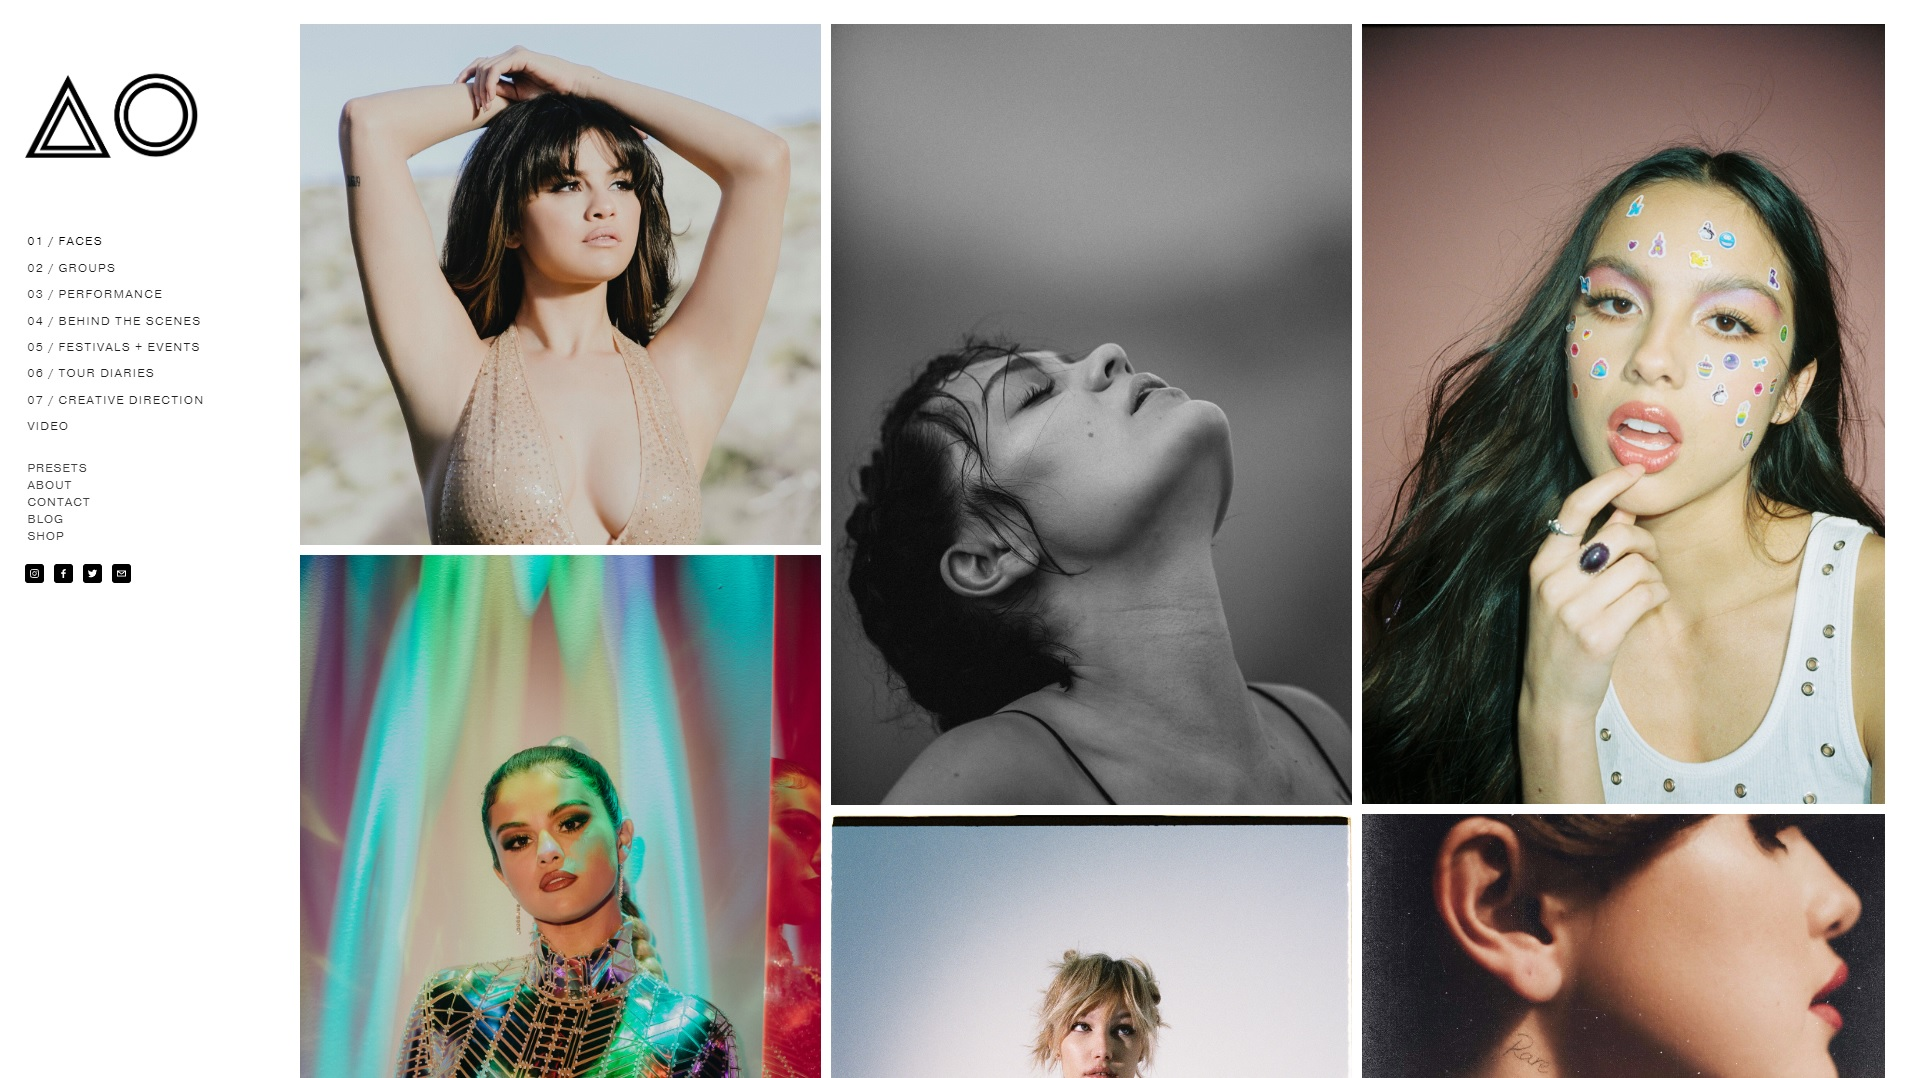
\includegraphics[width=0.95\textwidth]{images/ashley-1.jpg}}
   \caption{\textit{\url{www.ashleyosborn.com}} --- strona główna.}
   \label{fig:ashley-1.jpg}
\end{figure}

Rysunek \ref{fig:ashley-1.jpg} przedstawia wygląd strony głównej witryny internetowej \url{www.ashleyosborn.com}. Warto zwrócić szczególną uwagę na kilka jej elementów. W~lewym górnym rogu znajduje się logo będące inicjałami właścicielki analizowanej strony. Pełni ono funkcję estetyczną i jest ważną częścią identyfikacji wizualnej. Ponadto, będąc w dowolnym miejscu na stronie fotografki, można na nie kliknąć --- spowoduje to przeniesienie użytkownika na stronę główną. Oprócz logo, w lewej części strony umieszczone zostało menu, które też jest zawsze widoczne. Resztę, a zarazem większość ekranu, wypełniają zdjęcia. Warto zaznaczyć, że ich wybór nie jest przypadkowy --- osoby, które się na nich pojawiły, są znanymi na świecie artystkami. Przykładowo osoba pozująca na pierwszej fotografii od lewej to Selena Gomez - posiada ona największą liczbę (ponad 373 miliony) obserwujących na Instagramie \cite{instagram}. 

\begin{figure}[H] 
    \centering
         \fbox{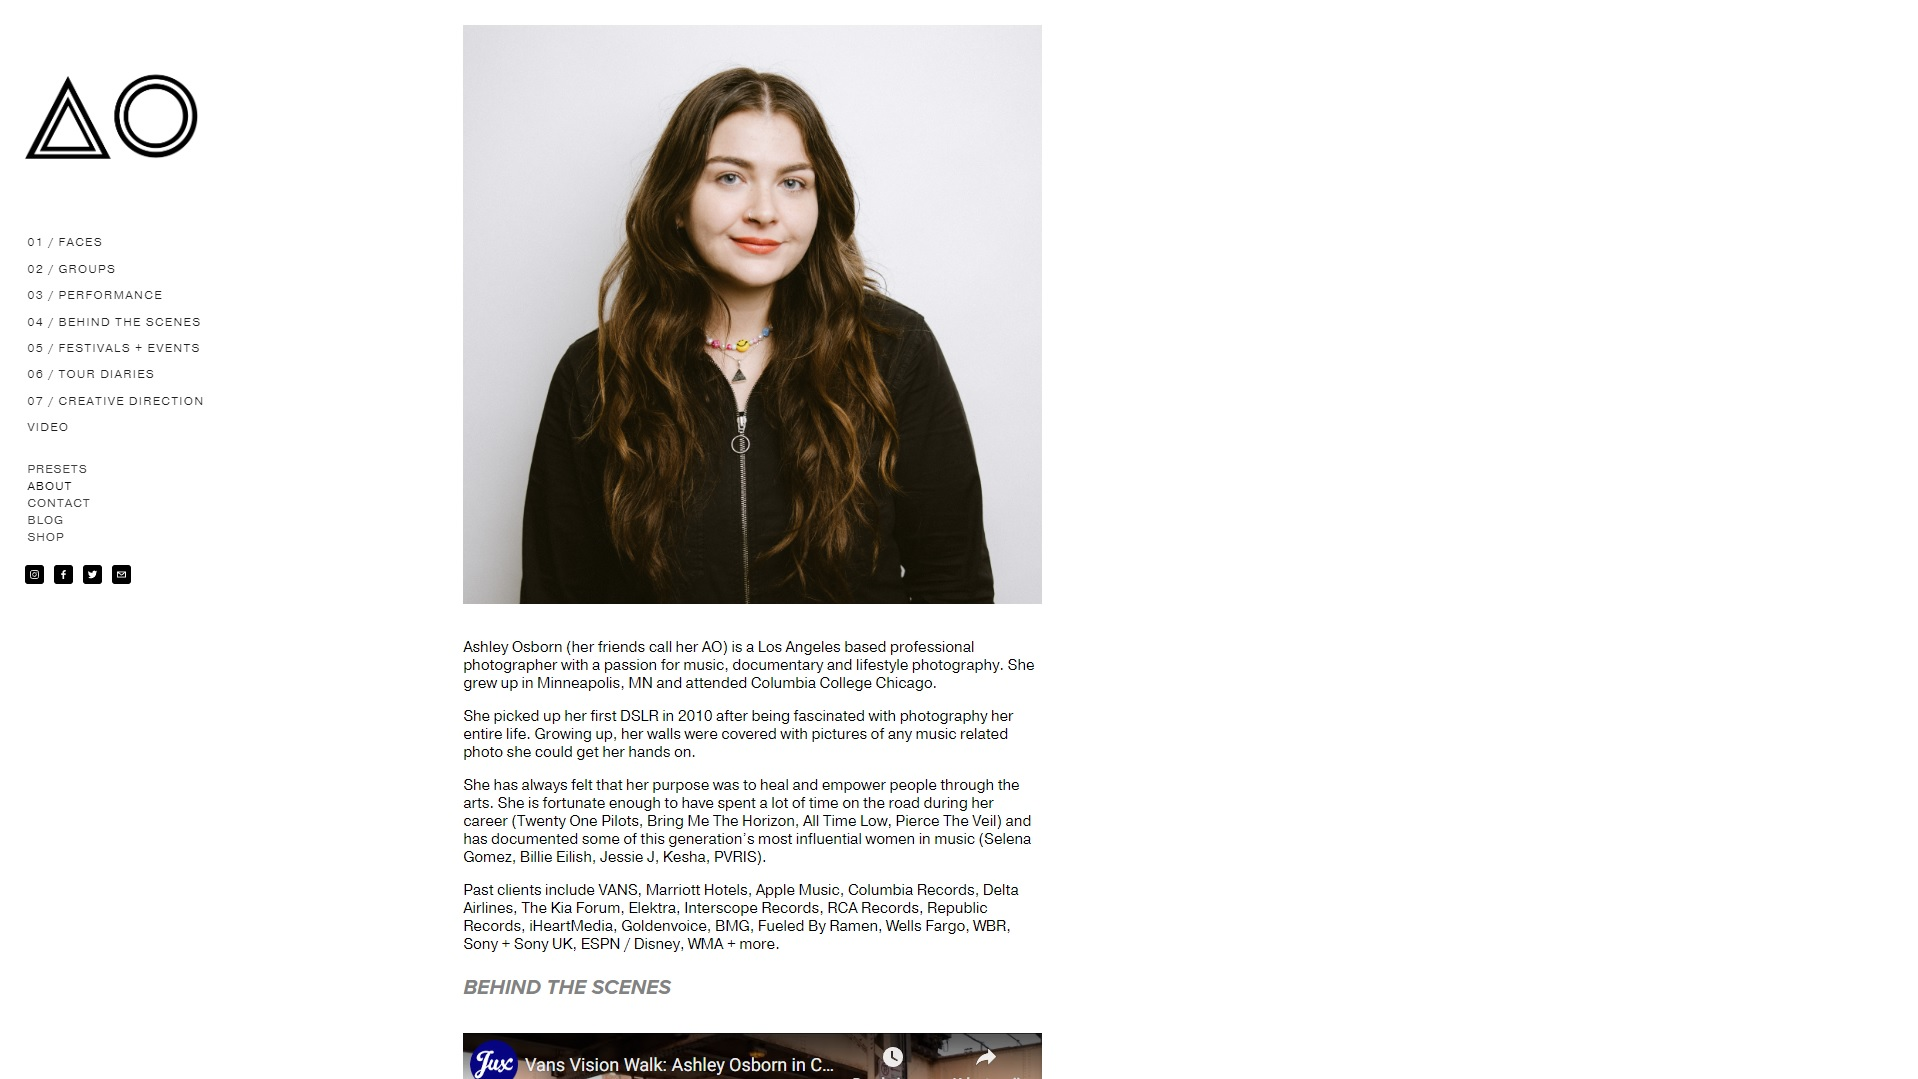
\includegraphics[width=0.95\textwidth]{images/ashley-2.jpg}}
   \caption{\textit{\url{www.ashleyosborn.com}} --- sekcja ``o mnie''.}
   \label{fig:ashley-2.jpg}
\end{figure}

\begin{figure}[H] 
    \centering
         \fbox{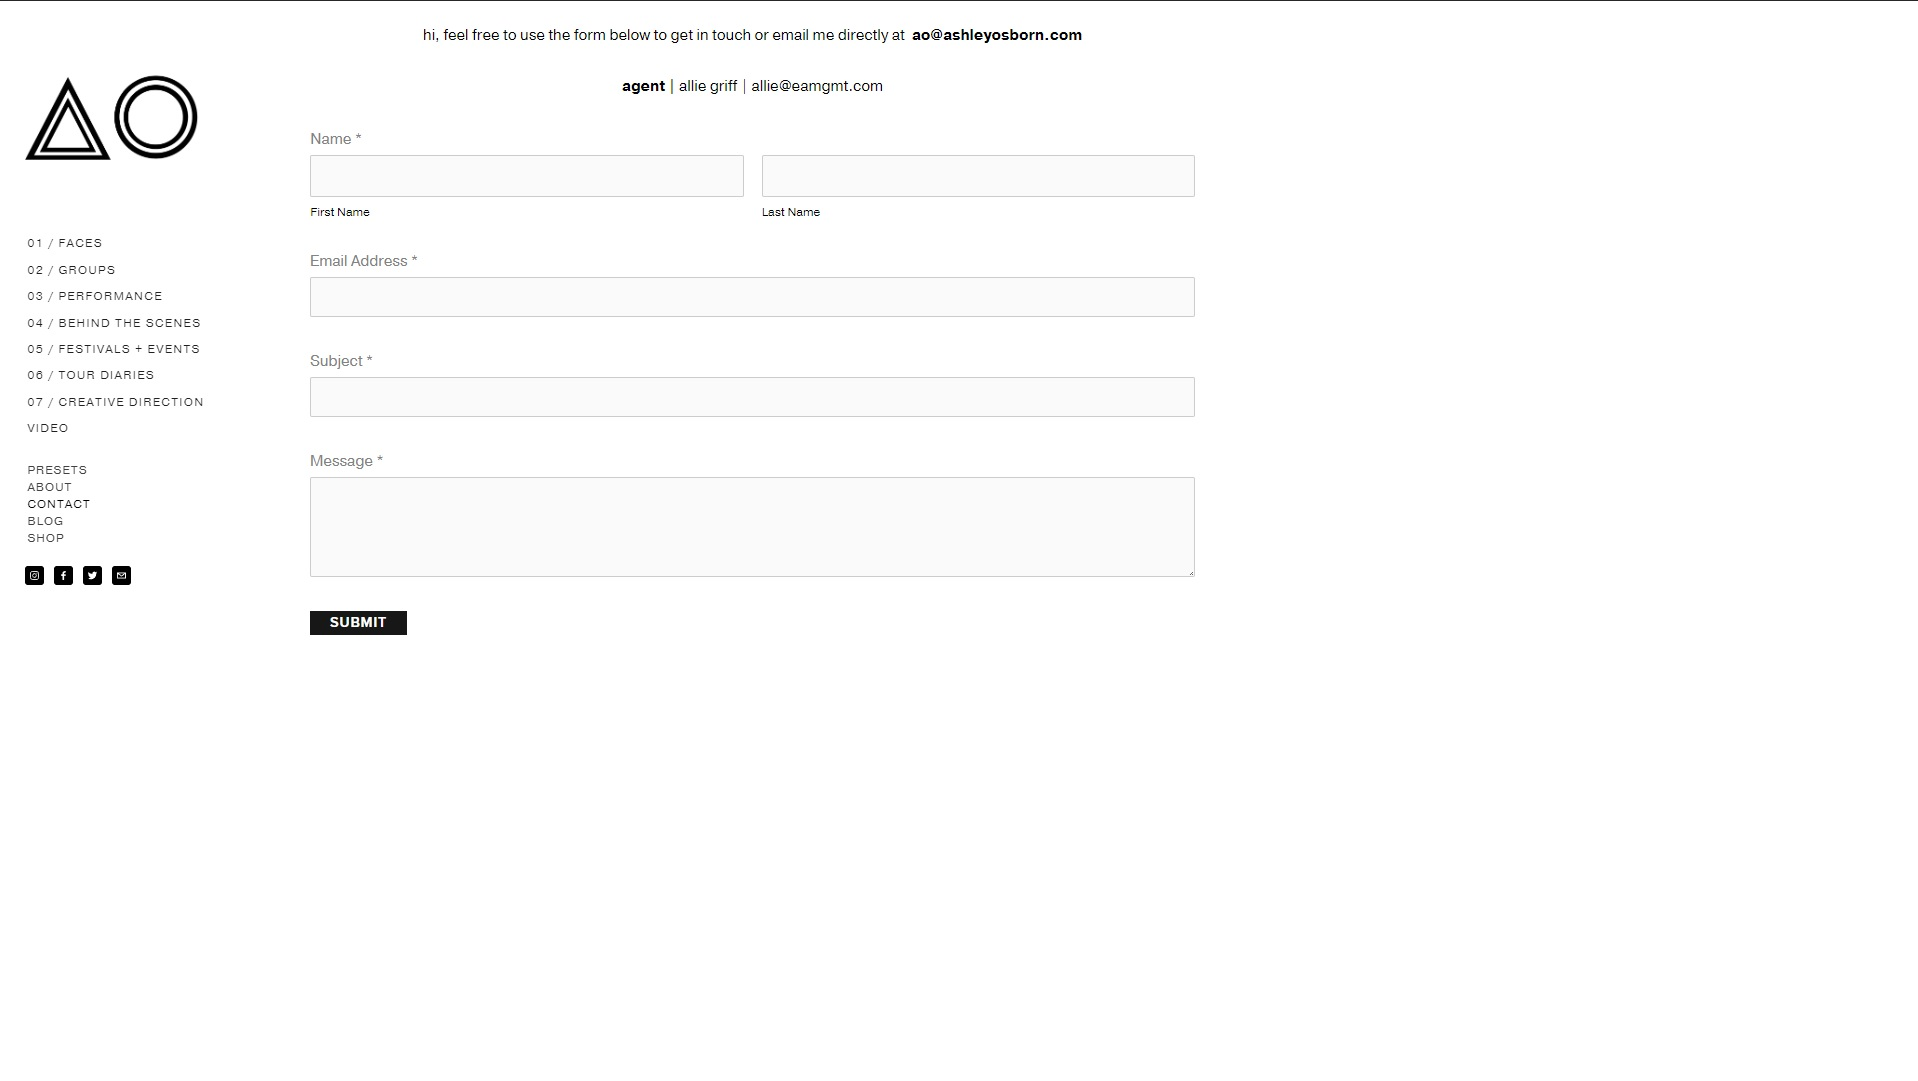
\includegraphics[width=0.95\textwidth]{images/ashley-3.jpg}}
   \caption{\textit{\url{www.ashleyosborn.com}} --- formularz kontaktowy.}
   \label{fig:ashley-3.jpg}
\end{figure}

\newpage

Widoczna na rysunku \ref{fig:ashley-2.jpg} sekcja ``o mnie'' jest kolejnym nieodłącznym elementem każdej strony-wizytówki należącej do osoby zajmującej się profesjonalną fotografią. Pozwala ona przedstawić wygląd, charakter i osiągnięcia osoby, która chce zachęcić potencjalnych klientów do skorzystania z usługi. Nie musi być ona rozbudowana --- w tym przypadku są to portret oraz krótki, lecz treściwy opis życiorysu Ashley Osborn. Zawiera on między innymi wykaz najważniejszych zleceń z przeszłości, nazwę ukończonej szkoły wyższej, a także obecne miejsce zamieszkania. Formularz kontaktowy z rysunku \ref{fig:ashley-3.jpg} umożliwia szybkie wysłanie wiadomości bez konieczności używania poczty elektronicznej lub mediów społecznościowych. Warto zwrócić uwagę na gwiazdki przy polach obowiązkowych (w tym przypadku --- po prostu wszystkich polach). Wprowadzane dane powinny być walidowane, a~użytkownik poinformowany zarówno wtedy, gdy próba wysłania danych powiedzie się, jak i wtedy, gdy wystąpi błąd \cite{formularze}. 

Ostatnią sekcją strony Ashley Osborn jest blog, skonstruowany w prosty sposób, podobny do reszty strony. Użytkownik może wybrać interesujący go post z~listy (rys. \ref{fig:ashley-4.jpg}), po czym przenoszony jest do jego treści (rys. \ref{fig:ashley-5.jpg}). Należy tu się przyjrzeć tekstowi --- nie zajmuje on całej szerokości strony. Ułatwia to czytanie - zarówno zbyt szerokie, jak i zbyt wąskie akapity skutecznie zniechęcają użytkownika do czytania \cite{szerokosc}. Oprócz rzeczy przedstawionych na powyższych zrzutach ekranu, na stronie istnieje też możliwość przejścia do sklepu, w którym sprzedawane są \textit{presety}\footnote{ang. preset --- zestaw gotowych ustawień, najczęściej wykorzystywany przy obróbce dużej liczby zdjęć, pozwalający na utrzymanie spójnej stylistyki na każdym z nich.} do programu do obróbki zdjęć Adobe Lightroom.

\begin{figure}[H] 
    \centering
         \fbox{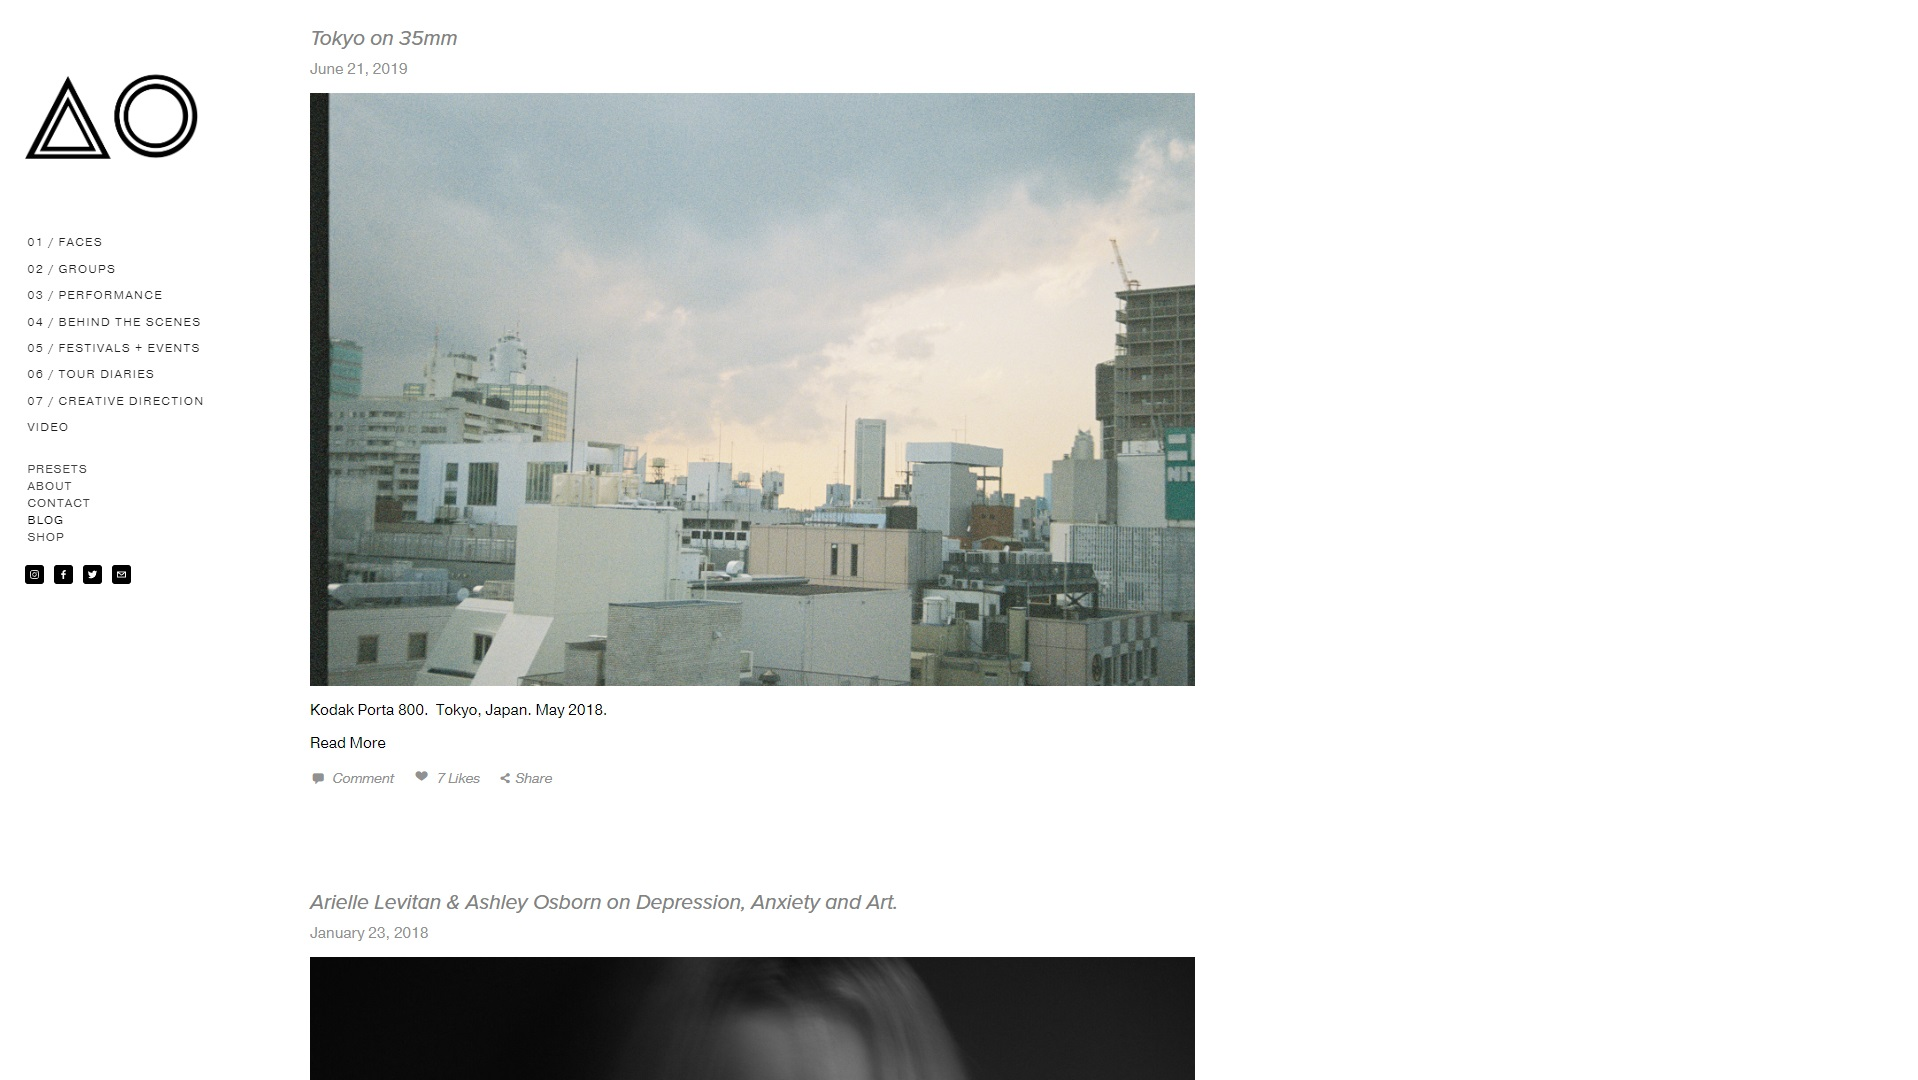
\includegraphics[width=0.95\textwidth]{images/ashley-4.jpg}}
   \caption{\textit{\url{www.ashleyosborn.com}} --- blog (lista postów).}
   \label{fig:ashley-4.jpg}
\end{figure}

\begin{figure}[H] 
    \centering
         \fbox{
\includegraphics[width=0.95\textwidth]{images/ashley-5.jpg}}
   \caption{\textit{\url{www.ashleyosborn.com}} --- blog (widok postu).}
   \label{fig:ashley-5.jpg}
\end{figure}


%%% Zackery Michael

\newpage

\subsubsection{Zackery Michael}

\begin{figure}[H] 
    \centering
         \fbox{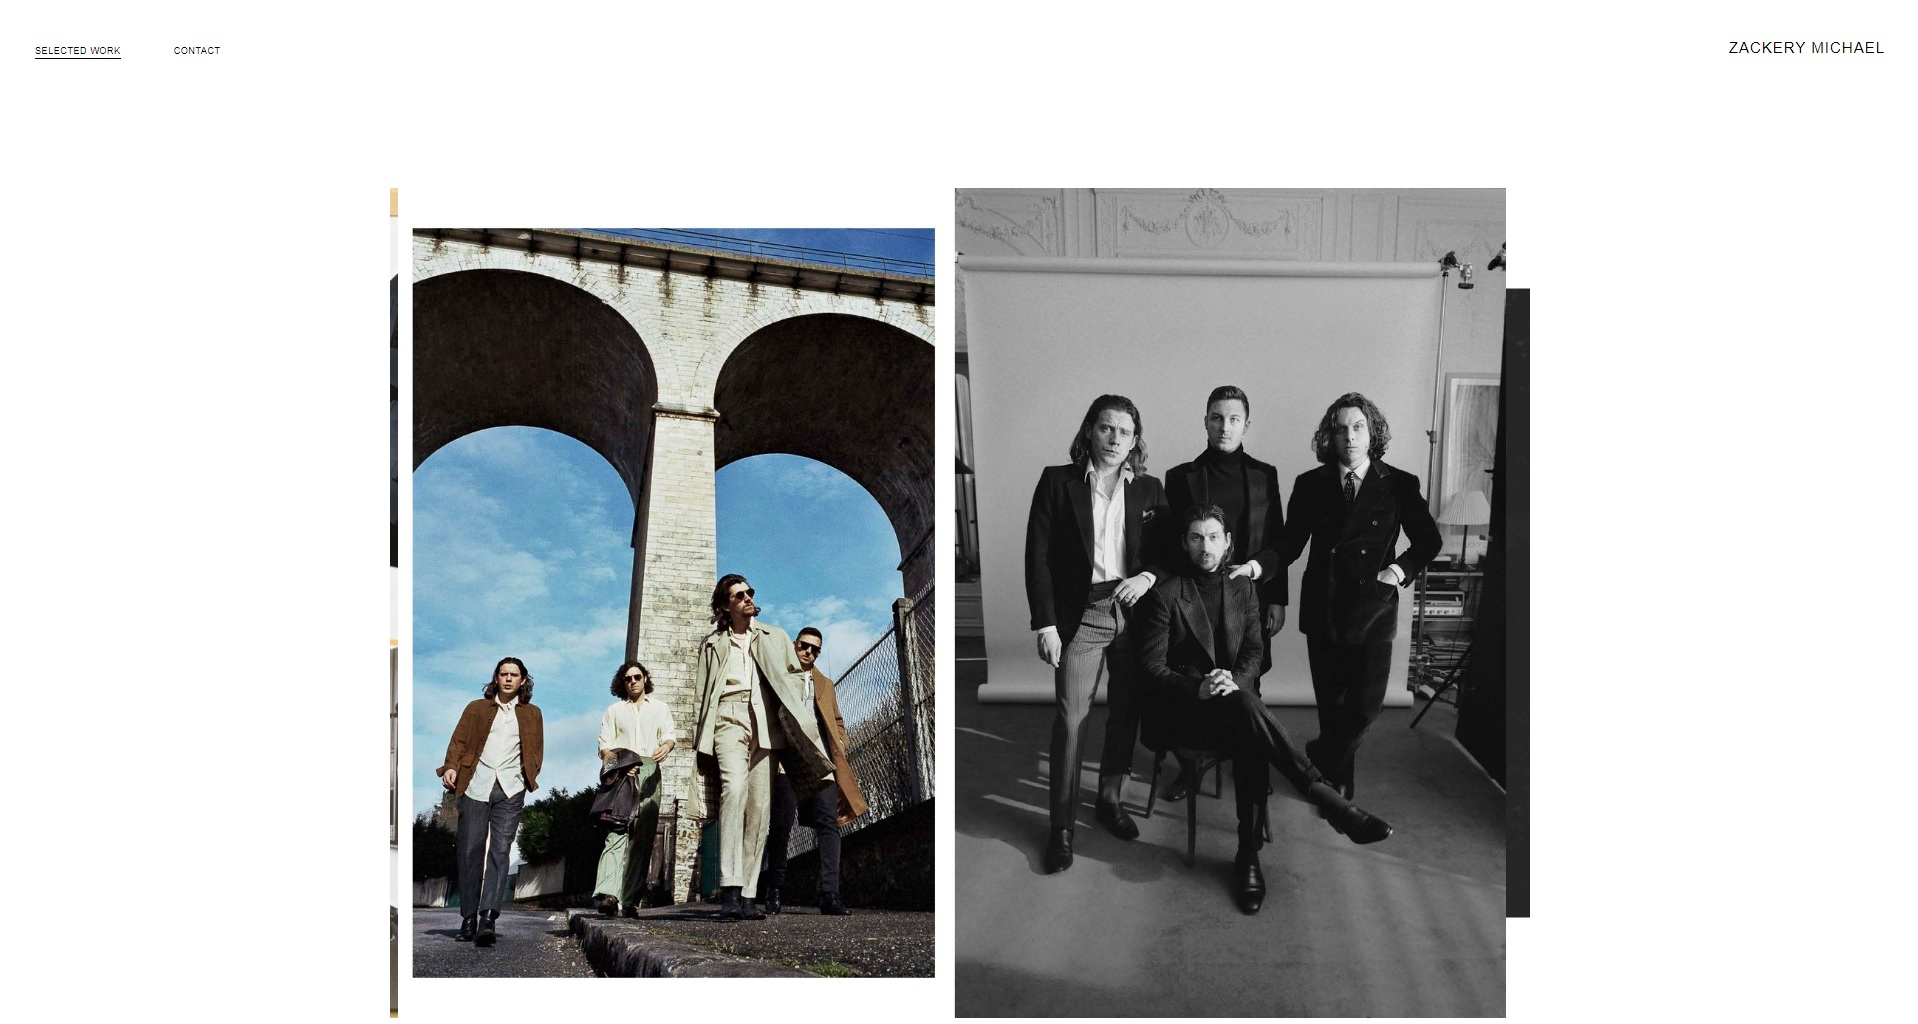
\includegraphics[width=0.95\textwidth]{images/zackery-1.jpg}}
   \caption{\textit{\url{www.zackerymichaelstudio.com}} --- strona główna.}
   \label{fig:zackery-1.jpg}
\end{figure}

\begin{figure}[H] 
    \centering
         \fbox{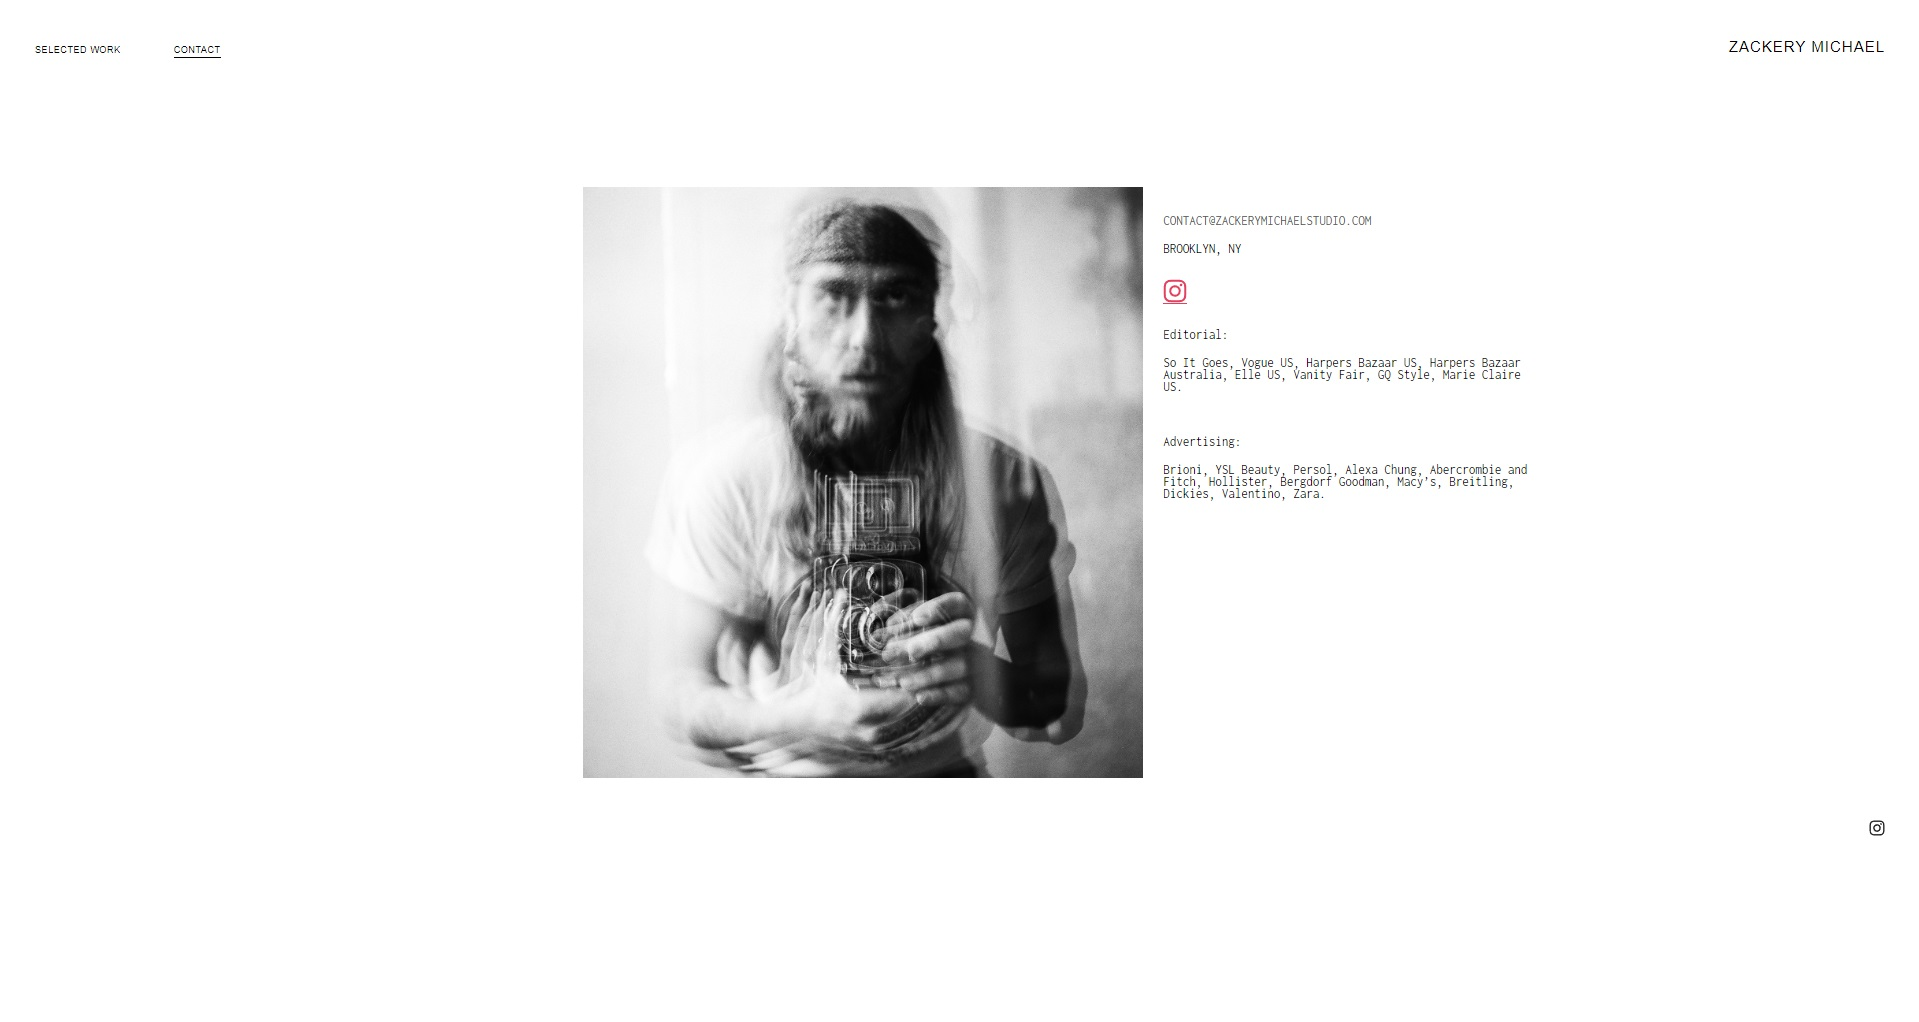
\includegraphics[width=0.95\textwidth]{images/zackery-2.jpg}}
   \caption{\textit{\url{www.zackerymichaelstudio.com}} --- sekcja kontaktowa.}
   \label{fig:zackery-2.jpg}
\end{figure}

Druga przedstawiona strona-wizytówka jest zupełnie inna w porównaniu do poprzedniej. O ile sam wygląd pierwszej analizowanej witryny był prosty, to ilość treści była dość bogata (blog, sekcja ``o mnie'', oddzielny formularz kontaktowy czy nawet sklep). W przypadku portfolio nowojorskiego fotografa Zackery'ego Michaela zastosowano zdecydowanie bardziej minimalistyczne podejście. Jego witryna internetowa składa się jedynie z dwóch części: strony głównej, przeznaczonej do zaprezentowania wybranych prac (rys. \ref{fig:zackery-1.jpg}) oraz sekcji ``kontakt'', gdzie obok zdjęcia przedstawiającego Zackery'ego Michaela podany jest jego adres poczty elektronicznej oraz przedstawione są najważniejsze firmy, z którymi współpracował fotograf (rys. \ref{fig:zackery-2.jpg}). Tekst jest znacznie ograniczony w celu zwrócenia pełnej uwagi odwiedzających stronę na prace zaprezentowane przez Zackery'ego Michaela.

%% Portale społecznościowe

\subsection{Portale społecznościowe}

Wraz z rozwojem technologii internetowych pojawiły się portale społecznościowe, które w dzisiejszych czasach pełnią bardzo ważną funkcję zarówno w znaczeniu społecznym (ułatwiają kontakt oraz zawieranie nowych znajomości przez Internet), jak i biznesowym (ze względu na wielką popularność są potężnym narzędziem marketingowym i źródłem pozyskiwania klientów). W~kontekście zawodu fotografa są one o tyle ważne, że Instagram oraz Facebook, czyli te najbardziej popularne, są w dużej mierze oparte na udostępnianiu zdjęć. Pomaga to w budowaniu marki osobistej osoby świadczącej usługi fotograficzne, co ułatwia zdobywanie nowych zleceń i poszerzanie działalności poza rynek lokalny \cite{socialmedia}. Wspomniane portale społecznościowe zostaną w tym rozdziale opisane pod kątem prezentacji treści, zwłaszcza postów (Facebook) i zdjęć (Instagram) oraz profilów użytkownika.

%%% Instagram

\subsubsection{Instagram}

Instagram to powstały w 2010 roku \cite{instagramfirstday} portal społecznościowy skupiony na możliwości udostępniania zdjęć i filmów, które następnie mogą być polubione\footnote{polubienie, potocznie lajk (ang. like) --- wyrażenie aprobaty wobec treści poprzez np. kliknęcie kciuka w górę lub symbolu serca.} oraz komentowane przez innych użytkowników. Wśród fotografów jego popularność jest szczególnie duża ze względu na możliwość pełnienia przez ten serwis funkcji portfolio oraz łatwość podjęcia kontaktu poprzez wiadomości bezpośrednie. Przykładowym zaprezentowanym profilem użytkownika będzie widoczny na rysunku \ref{fig:instagram-1.jpg} profil Ashley Osborn, fotografki, której strona internetowa została opisana w podrozdziale \ref{ashley}. Składa się on z kilku elementów, którymi są: 
\begin{itemize}
    \item Część nagłówkowa ze zdjęciem profilowym, informacjami o liczbie postów, osób obserwujących oraz obserwowanych, opisem profilu oraz linkiem do strony internetowej.
    \item Zapisane relacje (ang. \textit{stories} --- wprowadzony w 2016 roku mechanizm Instagrama, pozwalający na udostępnianie zdjęć oraz filmów znikających po 24 godzinach \cite{stories}).
    \item Galeria w postaci szerokiej na trzy elementy siatki kwadratowych zdjęć lub filmów. Warto zwrócić uwagę, że trzy pierwsze posty są przypięte, \linebreak  a kolejne --- ułożone w kolejności od najnowszych do najstarszych. Opcja przypinania postów daje użytkownikom większy wpływ na wygląd ich profilu poprzez wyróżnienie ulubionych zdjęć lub filmów.
\end{itemize}

\begin{figure}[H] 
    \centering
         \fbox{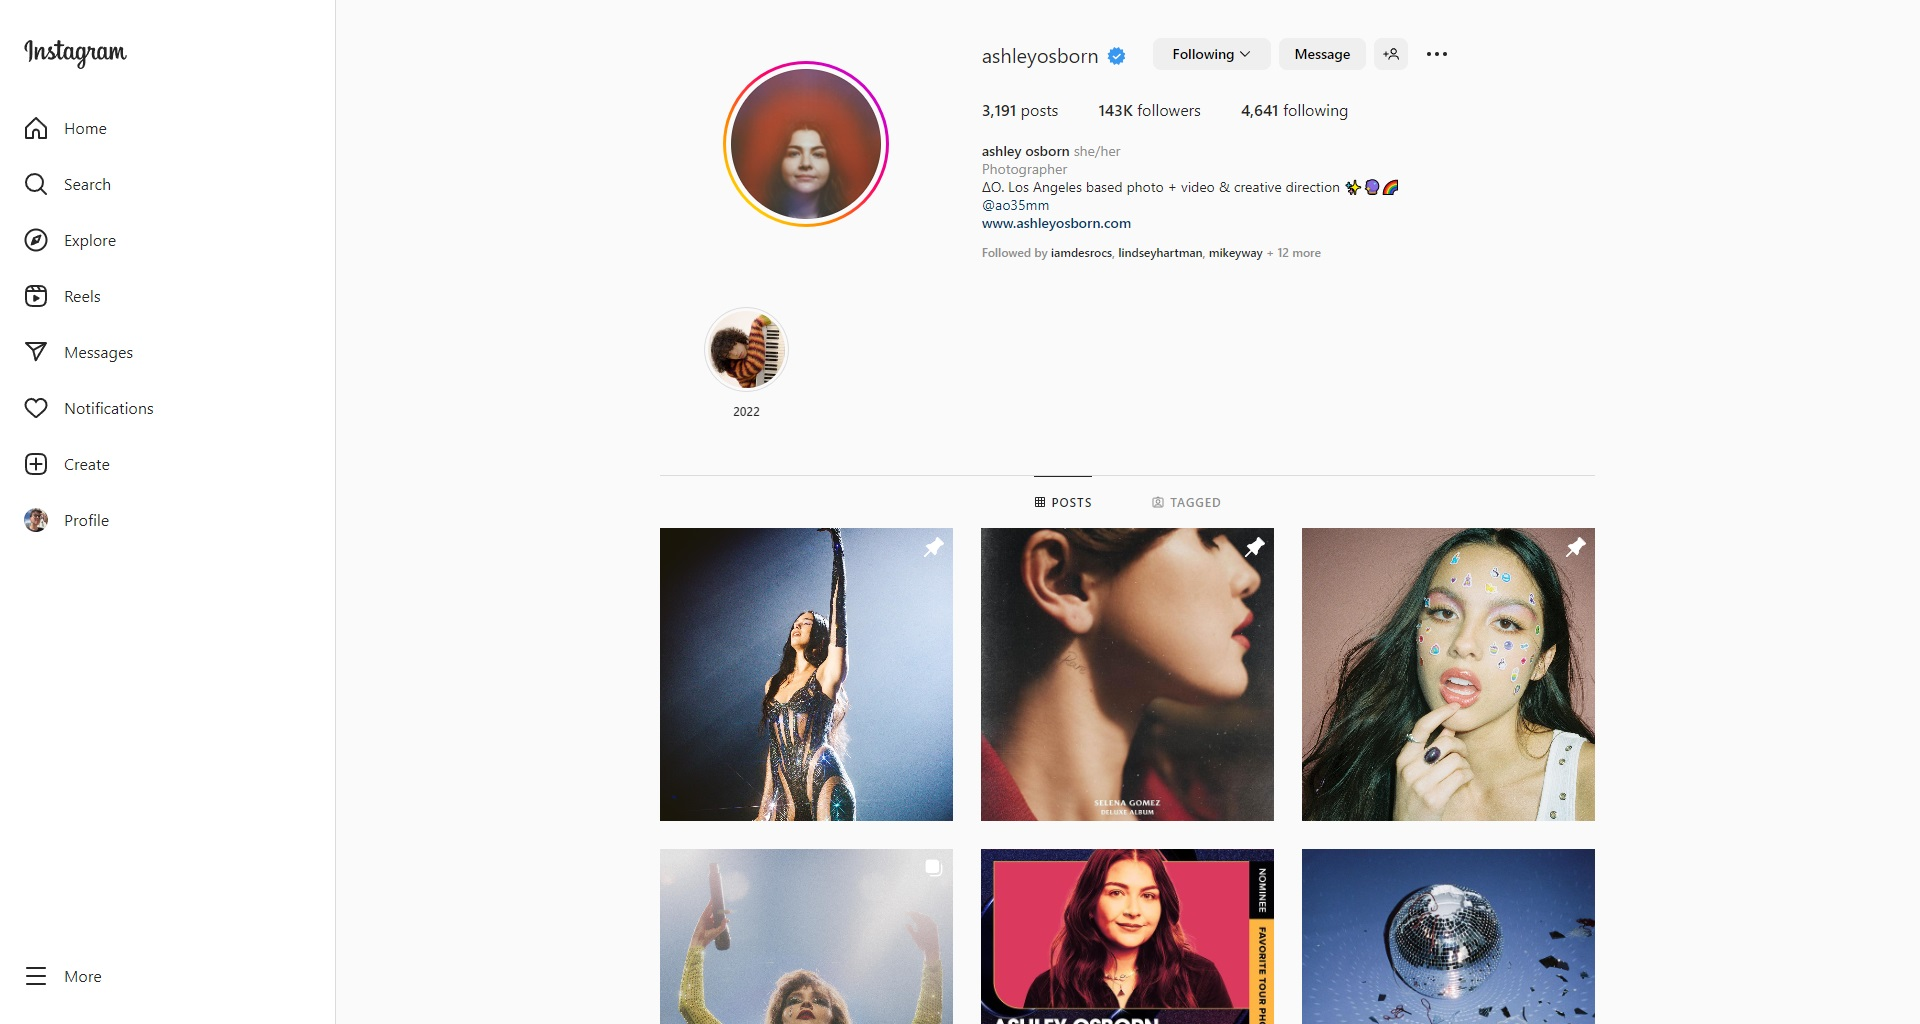
\includegraphics[width=0.95\textwidth]{images/instagram-1.jpg}}
   \caption{Instagram --- profil użytkownika.}
   \label{fig:instagram-1.jpg}
\end{figure}

\begin{figure}[H] 
    \centering
         \fbox{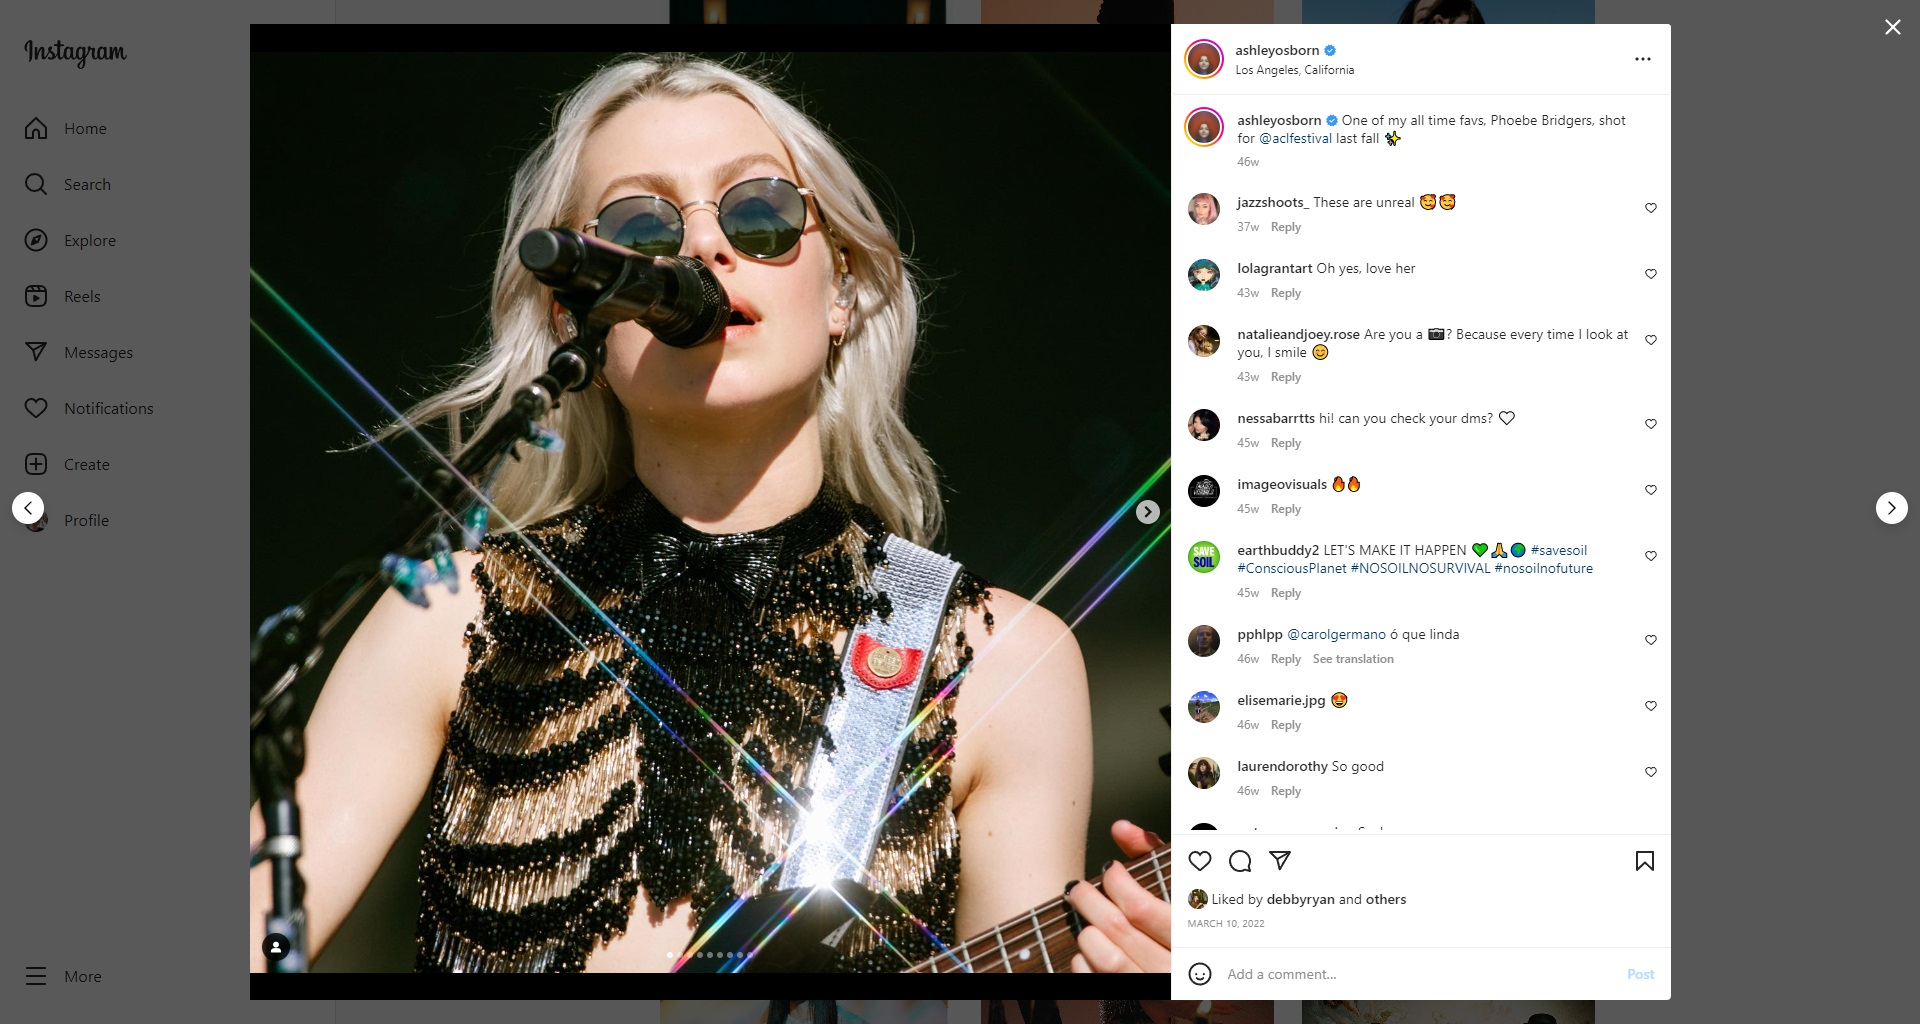
\includegraphics[width=0.95\textwidth]{images/instagram-2.jpg}}
   \caption{Instagram --- widok postu.}
   \label{fig:instagram-2.jpg}
\end{figure}

Kolejnym widokiem jest widok postu (rys. \ref{fig:instagram-2.jpg}). Pozwala on na przeglądanie wszystkich znajdujących się w nim filmów i zdjęć, czytanie i dodawanie komentarzy, polubienie postu oraz udostępnienie go za pomocą wiadomości prywatnej lub skopiowanie linku, aby umieścić go poza Instagramem. Warto zwrócić uwagę na przyciemnioną pozostałą część strony --- użytkownik po zamknięciu postu wróci do miejsca, od którego zaczął jego oglądanie. 

%%% Facebook

\subsubsection{Facebook}

Założony w 2004 roku \cite{historiafacebooka} Facebook to najpopularniejszy pod względem miesięcznej liczby użytkowników serwis społecznościowy \cite{socialmediastats}. Portal ten jest wykorzystywany zarówno do tworzenia profilów prywatnych, jak i firmowych. Użytkownicy mogą dodawać się nawzajem do grona znajomych, umieszczać na swojej tablicy posty tekstowe lub ze zdjęciami i filmami, tworzyć grupy, obserwować interesujące ich strony. Te ostatnie mogą reprezentować np. popularnych artystów, lokalne firmy lub po prostu umieszczać treści o określonej tematyce. Ze względu na ogromną popularność i idącym za nią potencjałem marketingowym posty publikowane przez strony mogą też być promowane, co zwiększa potencjalną liczbę odbiorców. Elementami profilu użytkownika są: 
\begin{itemize}
    \item część nagłówkowa zawierająca tło, zdjęcie profilowe, nazwę strony, liczbę osób obserwujących i obserwowanych, możliwość zaobserwowania profilu oraz opcję wyszukiwania (rys. \ref{fig:facebook-1.jpg});
    \item sekcja o nazwie ``Prezentacja'' --- krótki opis, informacja o rodzaju strony oraz odniesienie do strony internetowej (rys. \ref{fig:facebook-1.jpg});
    \item galeria zdjęć (rys. \ref{fig:facebook-2.jpg});
    \item uporządkowana chronologicznie (od najnowszego do najstarszego) lista postów (rys. \ref{fig:facebook-2.jpg}).
\end{itemize}
Posty mogą być wyświetlane oddzielnie. W zależności od tego, czy razem z nimi dodane jest zdjęcie lub film, widok ten się różni. Rysunek \ref{fig:facebook-3.jpg} przedstawia post ze zdjęciem, natomiast rysunek \ref{fig:facebook-4.jpg} --- post bez zdjęcia z osadzonym linkiem. Podobnie jak w przypadku strony prezentowanej w~podrozdziale \ref{ashley}, warto zwrócić uwagę na ograniczoną szerokość posta, a co za tym idzie --- tekstu.

\begin{figure}[H] 
    \centering
         \fbox{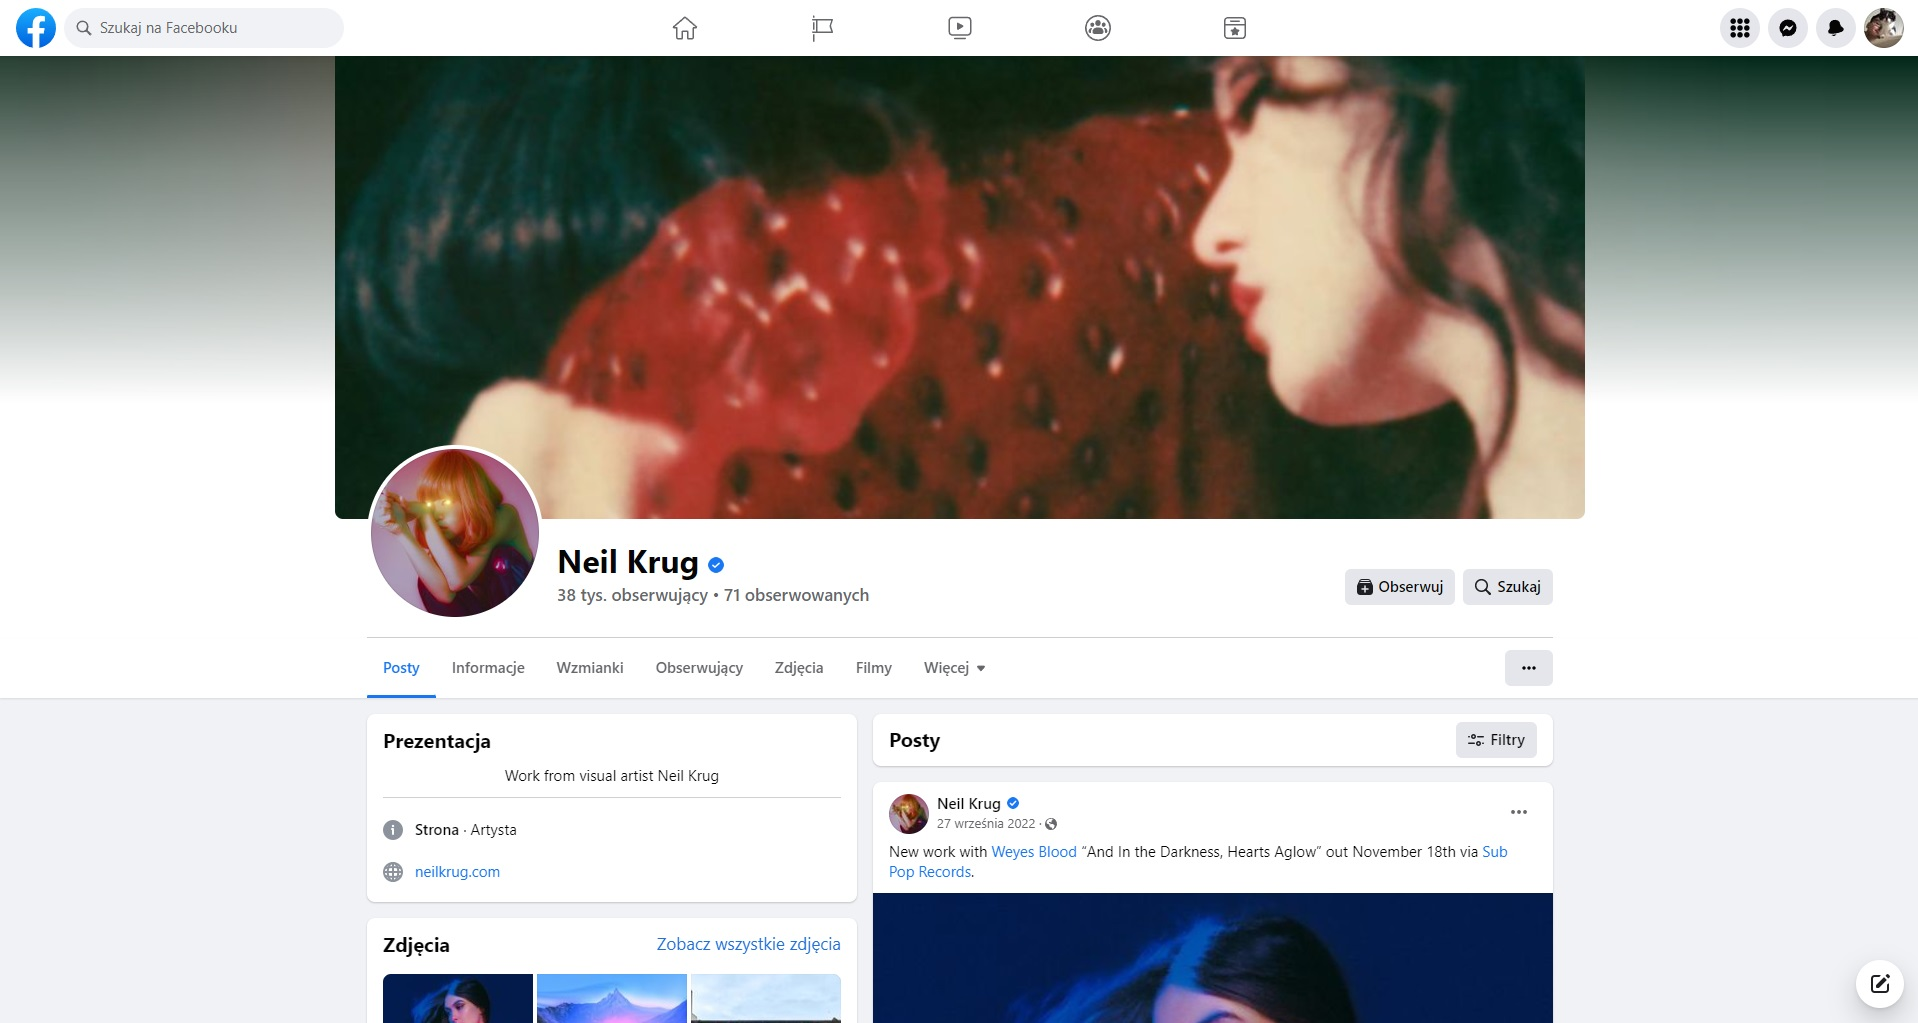
\includegraphics[width=0.95\textwidth]{images/facebook-1.jpg}}
   \caption{Facebook --- widok profilu użytkownika ze zdjęciem w tle.}
   \label{fig:facebook-1.jpg}
\end{figure}

\begin{figure}[H] 
    \centering
         \fbox{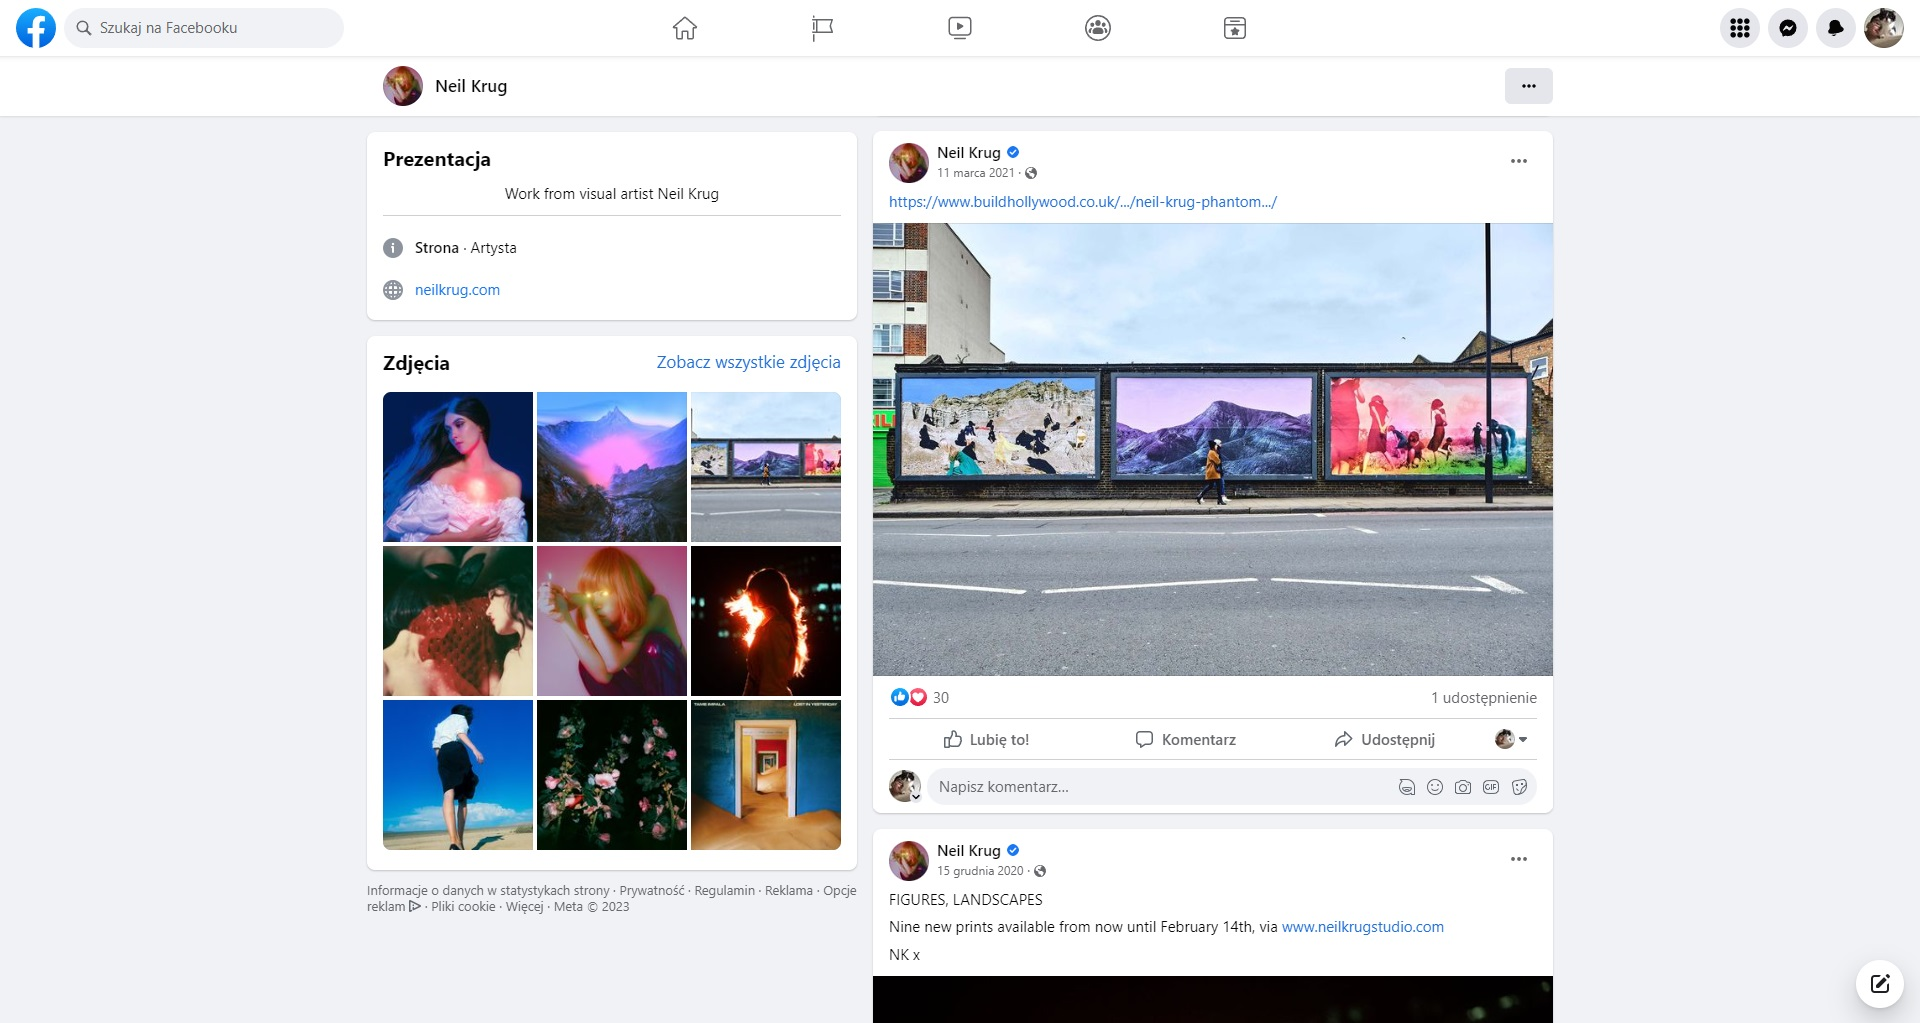
\includegraphics[width=0.95\textwidth]{images/facebook-2.jpg}}
   \caption{Facebook --- widok tablicy użytkownika po przewinięciu.}
   \label{fig:facebook-2.jpg}
\end{figure}

\begin{figure}[H] 
    \centering
         \fbox{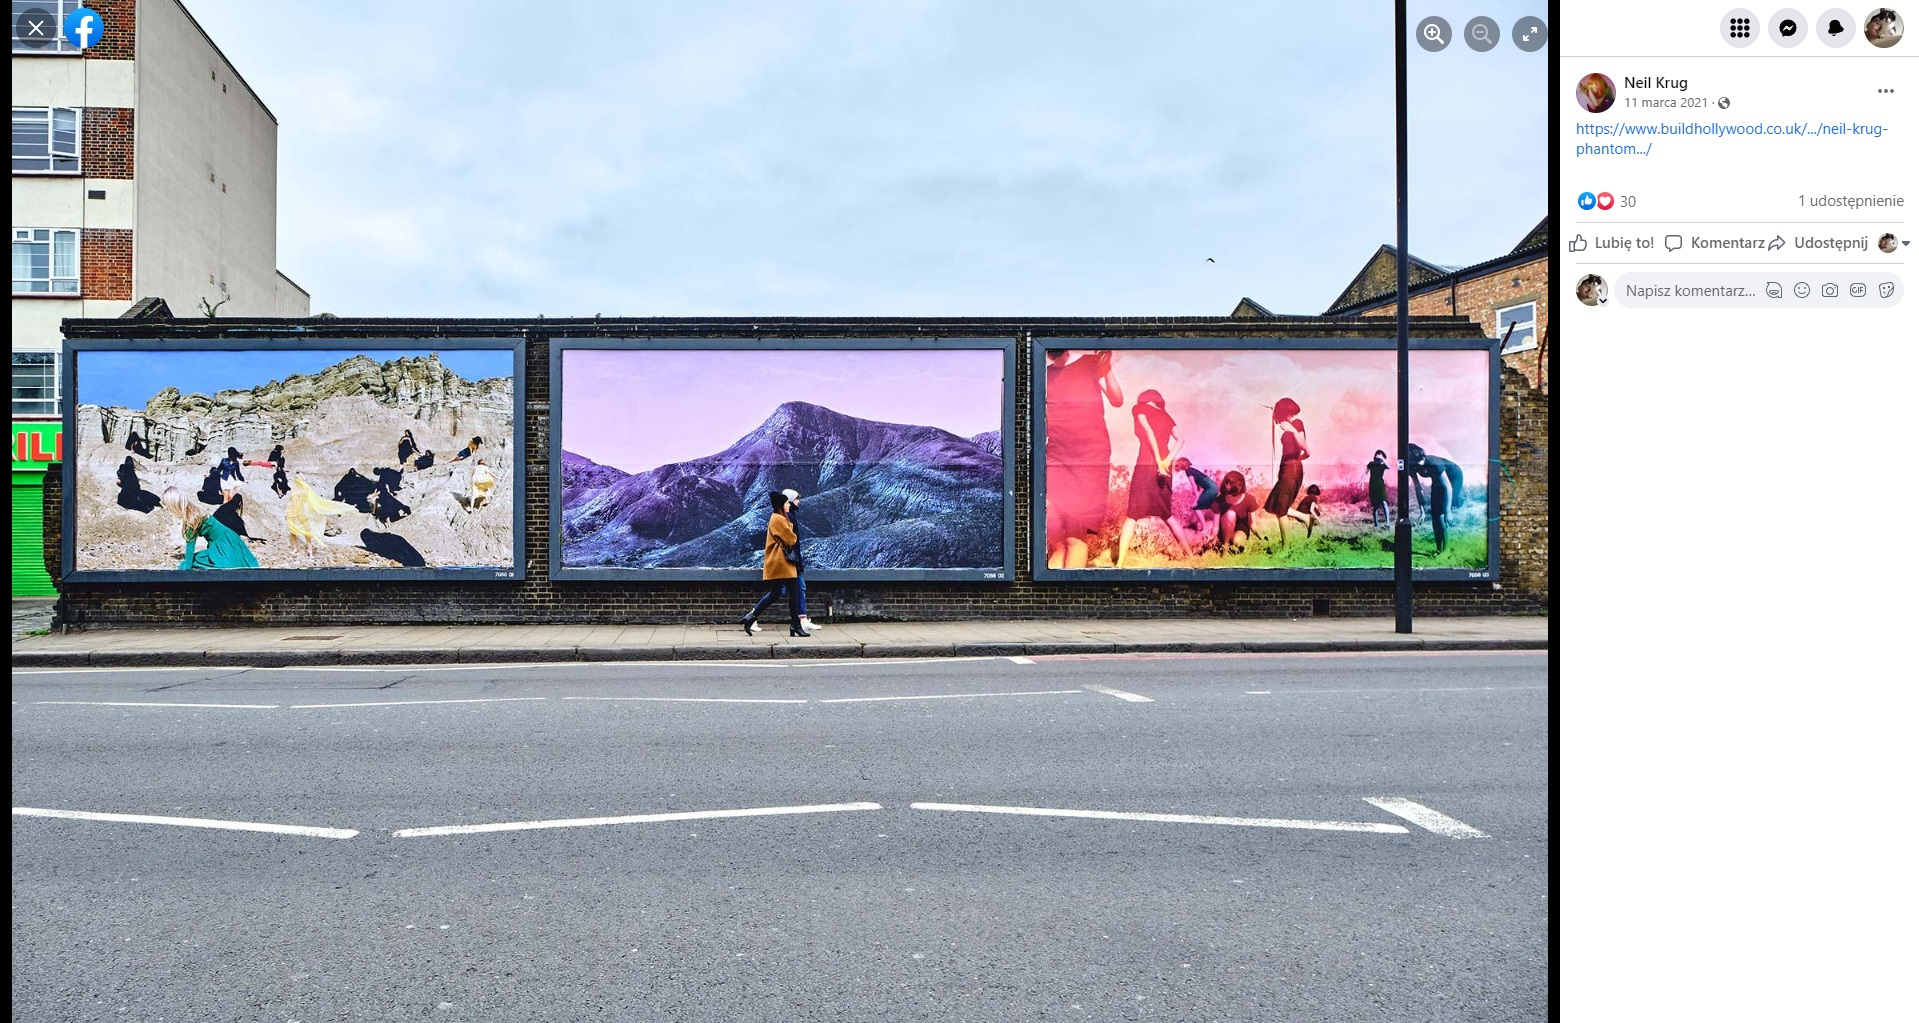
\includegraphics[width=0.95\textwidth]{images/facebook-3.jpg}}
   \caption{Facebook --- widok postu ze zdjęciem.}
   \label{fig:facebook-3.jpg}
\end{figure}

\begin{figure}[H] 
    \centering
         \fbox{
\includegraphics[width=0.95\textwidth]{images/facebook-4.jpg}}
   \caption{Facebook --- widok postu tekstowego (z osadzonym linkiem).}
   \label{fig:facebook-4.jpg}
\end{figure}

\subsection{Podsumowanie przeglądu}

Biorąc pod uwagę cechy analizowanych stron-wizytówek oraz portali społecznościowych używanych do pozyskiwania nowych klientów i promowania własnych prac, wyciągnięte zostały wnioski dotyczące podejścia do tworzenia projektu strony internetowej oraz planowania jej funkcjonalności. Po pierwsze, strony internetowe zawierające portfolio powinny być proste pod względem nawigacji (np. widoczny cały czas pasek nawigacyjny) oraz projektu graficznego (minimalistyczny układ i~prosta kolorystyka pozwalają skupić się na treści). Po drugie, w przypadku występowania większej ilości tekstu, wskazane jest zachowanie ograniczonej szerokości bloku tekstu. Strona główna jest pierwszym miejscem, w które trafia użytkownik, więc przydadzą się na niej skupiające uwagę zdjęcia (może to być spektakularna sceneria, ale też na przykład ktoś sławny). Sekcja ``o mnie'' powinna natomiast zawierać zwięźle opisany życiorys oraz doświadczenie zawodowe. W przypadku obecności formularza kontaktowego należy pamiętać o walidacji wprowadzanych przez użytkownika danych oraz wyświetlaniu rezultatu próby wysłania danych. W~czasach ogromnej popularności mediów społecznościowych dobrą praktyką jest też umieszczenie odnośników do znajdujących się tam profili fotografa.

% Narzędzia wybrane do realizacji projektu

\newpage 

\section{Narzędzia wybrane do realizacji projektu}

Niniejszy rozdział przedstawia narzędzia, które zostały wykorzystane do wykonania projektu graficznego tworzonej strony oraz jego realizacji. Ich wybór podyktowany był wcześniejszym doświadczeniem, dostępnością dokumentacji oraz dostosowaniem do wymagań projektowych, które zostały przedstawione w rozdziale~\ref{wymagania}.

%% Figma
\subsection*{Figma}

\begin{figure}[H] 
    \centering
        
\includegraphics[width=0.1\textwidth]{images/figma-logo.png}
   \caption{Logo narzędzia Figma.}
\end{figure}


\begin{figure}[H] 
    \centering
         \fbox{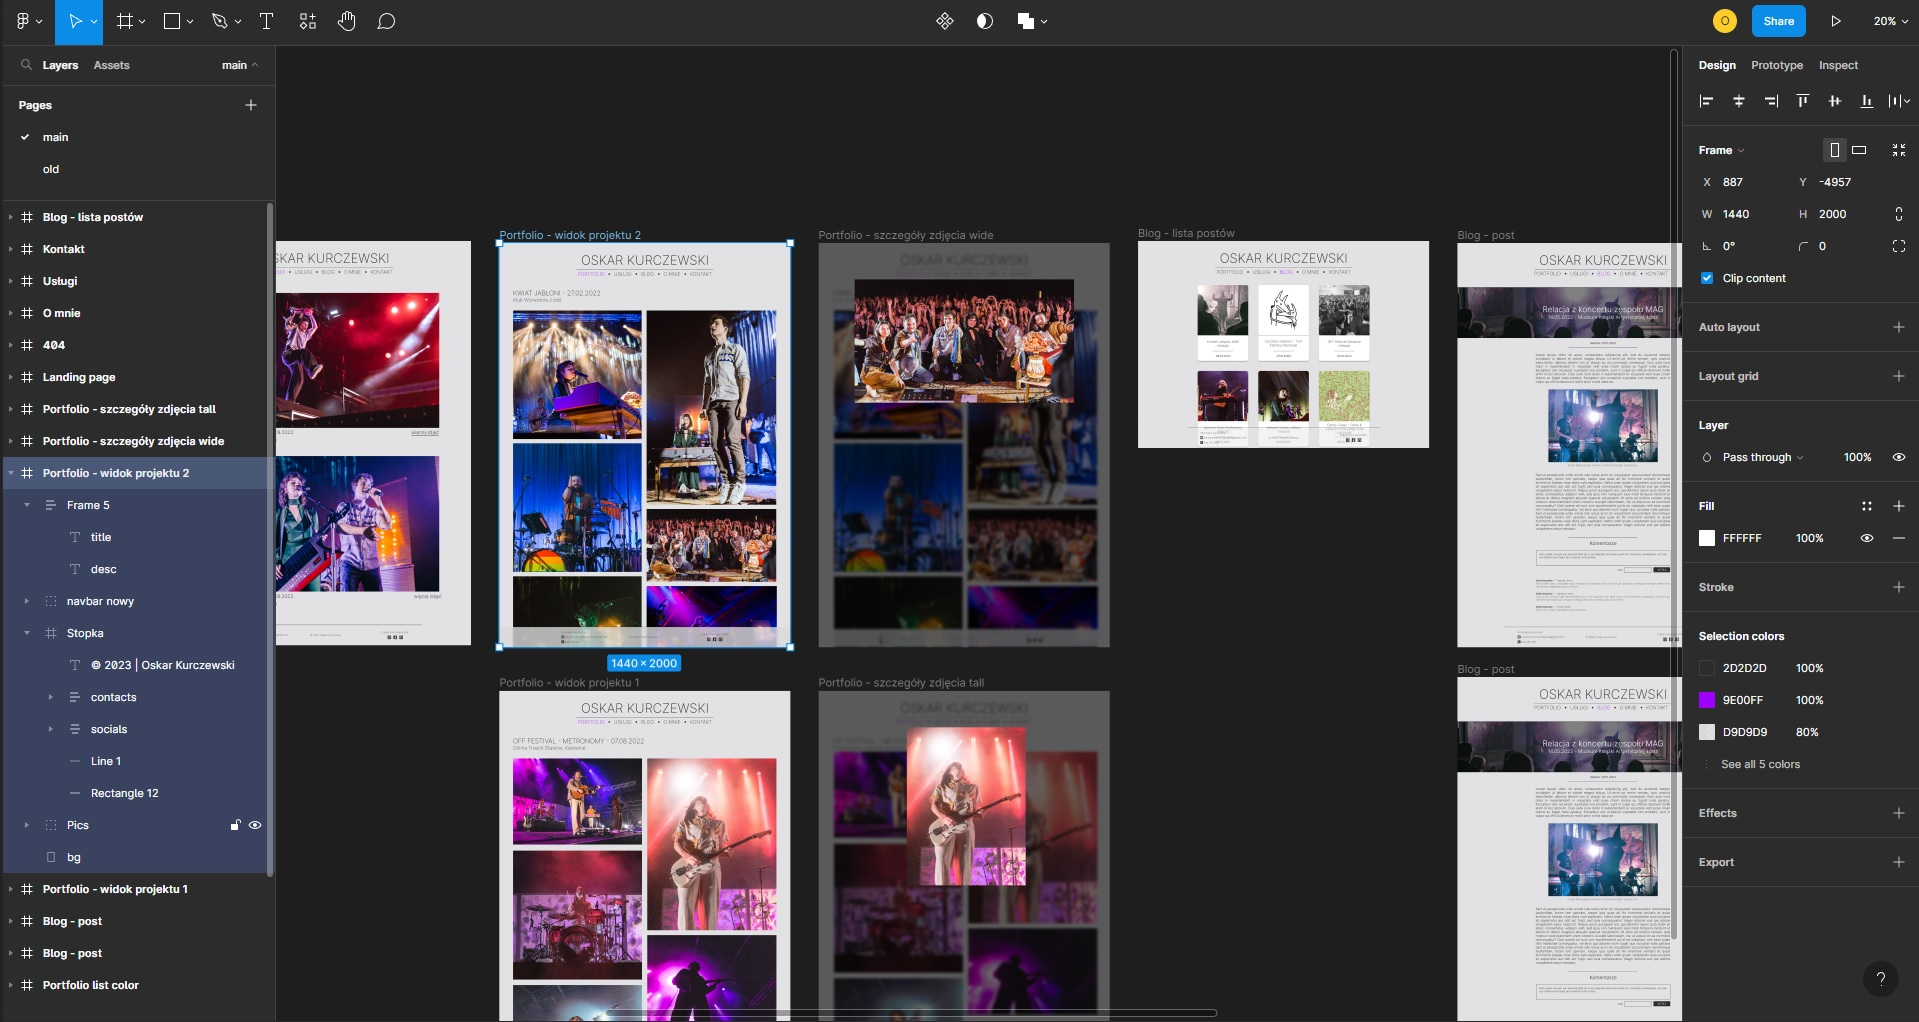
\includegraphics[width=0.95\textwidth]{images/figma-1.jpg}}
   \caption{Interfejs użytkownika narzędzia Figma.}
   \label{fig:figma-1.jpg}
\end{figure}

Wcześniejsze wykonanie projektu graficznego tworzonej strony internetowej pozwala na jej łatwiejszą implementację. Taki interfejs użytkownika jest też bardziej spójny wizualnie, co jest ważne dla pozytywnego odbioru strony. Do sporządzenia projektu strony-portfolio z blogiem wykorzystane zostało narzędzie Figma (rys.~\ref{fig:figma-1.jpg}) --- prosty w obsłudze program pozwalający na wykonanie interaktywnych projektów interfejsów użytkownika za pomocą grafiki wektorowej \cite{figma}. 

%% JavaScript

\subsection*{JavaScript}

\begin{figure}[H] 
    \centering
        
\includegraphics[width=0.1\textwidth]{images/js-logo.png}
   \caption{Logo języka JavaScript.}
\end{figure}

Przy implementacji tworzonego projektu wykorzystany został JavaScript~(JS), czyli najpopularniejszy język programowania na świecie \cite{js}. Cechują go: wieloplatformowość, wysokopoziomowość i dynamiczne typowanie. Jako zaletę języka JavaScript można wymienić wsparcie dla wielu platform --- tworzone za jego pomocą aplikacje mogą być używane zarówno na urządzeniach mobilnych, jak~i~w~przeglądarce. Ponadto duży wybór bibliotek oraz szkieletów aplikacyjnych ułatwia dobranie odpowiednich narzędzi do danego typu projektu.

%% Node/NPM

\subsection*{Node.js oraz npm}

\begin{figure}[H] 
    \centering
        
\includegraphics[width=0.1\textwidth]{images/node-logo.png}\hspace{16pt}
        
\includegraphics[width=0.1\textwidth]{images/npm-logo.png}
    \caption{Logotypy Node.js oraz npm.}
\end{figure}

Node.js to wieloplatformowe środowsko uruchomieniowe zbudowane w języku JavaScript \cite{node}. Jego działanie jest oparte na zdarzeniach asynchronicznych, dzięki czemu aplikacja stworzona w Node.js działa jako jeden proces. Integralnym elementem środowiska Node.js jest npm (\textit{Node Package Manager}) --- system zarządzania pakietami pozwalający na łatwą instalację wybranych bibliotek i narzędzi \cite{npm}. 

%% Strapi

\subsection*{Strapi}

\begin{figure}[H] 
    \centering
        
\includegraphics[width=0.2\textwidth]{images/strapi-logo.png}
   \caption{Logo systemu zarządzania treścią Strapi.}
\end{figure}

Strapi to system zarządzania treścią (CMS) typu \textit{headless} --- oznacza to, że nie pozwala on na definiowanie układu i wyglądu strony, a jedynie za zarządzanie treścią i jej dostarczanie do warstwy widoku. Użytkownik za pomocą intuicyjnego interfejsu graficznego może stworzyć model danych dostosowany do aktualnych potrzeb i wymagań. Do dyspozycji są dostępne typy pojedyncze (występujące tylko raz na całej stronie, np. treść sekcji ``o mnie''), kolekcje (np. posty lub projekty w portfolio) oraz komponenty (elementy powtarzające się w kolekcjach i typach pojedynczych) \cite{strapifeatures}. Głównymi zaletami Strapi są:
\begin{itemize}
    \item wsparcie dla wielu systemów zarządzania bazami danych --- SQLite (domyślny), MySQL, PostgresQL oraz MariaDB;
    \item wiele dostępnych wtyczek ułatwiających korzystanie z systemu;
    \item konfigurowalne API, pozwalające na dostosowanie systemu do potrzeb;
    \item obsługa kont użytkownika i uprawnień poprzez role, dzięki czemu nie ma konieczności jej oddzielnego implementowania.
\end{itemize}


%% SQLite

\subsection*{SQLite}

\begin{figure}[H] 
    \centering
        
\includegraphics[width=0.1\textwidth]{images/sqlite-logo.png}
   \caption{Logo systemu zarządzania bazami danych SQLite.}
\end{figure}

SQLite jest domyślnym systemem zarządzania relacyjną bazą danych dla Strapi. W porównaniu do innych popularnych systemów takich jak MySQL czy PostgresQL, SQLite wyróżnia się tym, że jest biblioteką języka C i nie wymaga oddzielnego procesu --- zapis i odczyt wykonywany jest po prostu za pomocą pliku bazy danych \cite{sqlite}. Dzięki temu jego ogromną zaletą są brak konieczności instalacji oraz konfiguracji bazy danych, a co za tym idzie --- łatwość użytkowania. SQLite wspiera język zapytań SQL (ang. \textit{Structured Query Language}).

%% React

\subsection*{React}

\begin{figure}[H] 
    \centering
        
\includegraphics[width=0.1\textwidth]{images/react-logo.png}
   \caption{Logo biblioteki React.}
\end{figure}

React to biblioteka będąca jednym z najpopularniejszych narzędzi do~tworzenia interfejsów użytkownika stron internetowych \cite{react}. Całość kodu pisana jest w JavaScripcie. Ważnym elementem Reacta jest JSX (ang. \textit{JavaScript Syntax Extension}) --- rozszerzenie składni JavaScript podobne do języka znaczników HTML. Ułatwia ono intuicyjne tworzenie komponentów, z których składa się strona internetowa.

%% Next.js

\subsection*{Next.js}

\begin{figure}[H] 
    \centering
        
\includegraphics[width=0.1\textwidth]{images/next-logo.png}
   \caption{Logo szkieletu aplikacyjnego Next.js.}
\end{figure}

Next.js jest szkieletem aplikacyjnym dla biblioteki React pozwalającym na tworzenie statycznych aplikacji internetowych \cite{next}. Jego kluczową cechą jest możliwość renderowania i generowania zawartości strony internetowej po~stronie serwera, co ulepsza pozycjonowanie witryny w wyszukiwarkach (SEO --- ang. \textit{search engine optimization}). Dla ułatwienia pracy nad tworzonymi stronami internetowymi, Next.js korzysta z routingu opartego na stronach. Dodatkowo, wsparcie dla routingu dynamicznego zapewnia m. in. możliwość łatwego tworzenia czytelnych dla użytkownika linków w formie unikalnego ciągu znaków (ang. \textit{slug}). Next.js posiada także integrację z Sassem --- preprocesorem języka CSS.

%% SCSS

\subsection*{Sass (SCSS)}

\begin{figure}[H] 
    \centering
        
\includegraphics[width=0.1\textwidth]{images/sass-logo.png}
   \caption{Logo preprocesora Sass.}
\end{figure}

Sass (ang. \textit{Syntactically Awesome Style Sheets}) to preprocesor i rozszerzenie języka CSS (ang. \textit{Cascading Style Sheets}) posiadający dodatkowe funkcjonalności takie, jak zmienne lub możliwość zagnieżdżania stylów w sposób odwzorowujący hierarchię występującą w HTML. SCSS (ang. \textit{Sassy CSS}) jest natomiast składnią będącą nadzbiorem CSS, co oznacza, że poprawnie napisany CSS może być jednocześnie wykorzystany w pliku SCSS \cite{sass}. Różnice pomiędzy składniami SASS oraz SCSS zostały zaprezentowane w~listingach \ref{chapter3:sass} i \ref{chapter3:scss}. Do realizacji projektu wybrana została składnia SCSS.\newline
\begin{code}[htbp]
    \lstinputlisting{./code/sass_example.txt}
    \caption
    [Przykład składni Sass.]
    {Przykład składni Sass.}
    \label{chapter3:sass}
\end{code}

\begin{code}[htbp]
    \lstinputlisting{./code/scss_example.txt}
    \caption
    [Przykład składni SCSS.]
    {Przykład składni SCSS.}
    \label{chapter3:scss}
\end{code}

% Projekt portfolio i blogu

\clearpage

\section{Projekt portfolio i blogu} \label{wymagania}
W tym rozdziale przedstawione zostaną założenia i wymagania (z podziałem na funkcjonalne i niefunkcjonalne) dotyczące projektu portfolio i blogu z systemem komentowania. W podrozdziale \ref{realizacja} wraz z fragmentami kodu źródłowego zaprezentowane będą również najważniejsze aspekty implementacji tworzonej strony internetowej.
 
%% Założenia projektu

\subsection{Założenia projektu}

Założenia projektu określają wizję tworzonego projektu oraz cel jego realizacji. Tworzona w ramach pracy inżynierskiej strona-wizytówka będzie składać się z~dwóch części --- systemu zarządzania treścią Strapi oraz odpowiedzialnej za warstwę widoku aplikacji stworzonej z wykorzystaniem szkieletu aplikacyjnego Next.js. Jej głównym zadaniem jest przedstawienie prac fotografa-dziennikarza muzycznego w formie portfolio z podziałem na projekty (np. konkretne sesje zdjęciowe lub wydarzenia) oraz udostępnienie w~formie bloga przestrzeni do wypowiedzi na temat powiązany z głównym obszarem tematycznym zdjęć, którym jest muzyka na żywo. Zgodnie z wnioskami z rozdziału \ref{przeglad}, graficzny interfejs tworzonej strony powinien być minimalistyczny, lecz nie surowy, co ma za zadanie skupić uwagę użytkownika na jej treści --- postach oraz fotografiach. 

%% Wymagania funkcjonalne

\subsection{Wymagania funkcjonalne}

Wymagania funkcjonalne określają konkretne funkcje, które powinny znaleźć się w tworzonej aplikacji internetowej, aby założenia projektu zostały spełnione. Skupiają się na sposobie działania jego poszczególnych elementów, pełnią funkcję listy tego, co powinno zostać zaimplementowane \cite{wymagania}. 

\subsubsection*{Dostęp do systemu zarządzania treścią}

Możliwość dodawania, edytowania i usuwania elementów powinna być zarezerwowana tylko dla osoby zarządzającej stroną internetową, wyłącznie za pomocą panelu administratora. Wyjątkiem są komentarze do postów oraz wpisy kontakowe, które mogą być dodawane za pomocą udostępnionego przez system REST API przez każdego użytkownika odwiedzającego stronę. 

\subsubsection*{Struktura danych w systemie zarządzania treścią} \label{struktura}

Struktura danych w systemie zarządzania treścią powinna być zorganizowana zgodnie z układem strony. Ułatwi to późniejsze pobieranie danych, a~także dodawanie oraz modyfikację treści. Potrzebne będą następujące kolekcje (elementy występujące na stronie więcej, niż jeden raz):
\begin{itemize}
    \item Post --- posiada tytuł, opis, miniaturkę i tło w formie zdjęć, treść złożoną z~dowolnej ilości akapitów i obrazów oraz kategorię (typ wyliczeniowy); może mieć dowolną ilość komentarzy.
    \item Wpis kontaktowy --- zawiera dane podane przez użytkownika (imię, nazwisko, adres poczty elektronicznej) oraz wiadomość i jej temat.
    \item Projekt --- posiada tytuł, opis, dowolną ilośc zdjęć oraz miniaturkę.
    \item Usługa --- posiada nazwę, opis, zdjęcie oraz cenę.
\end{itemize}
Na stronie pojawią się również elementy występujące wyłącznie jeden raz, dlatego wskazane będzie też stworzenie typów pojedynczych:
\begin{itemize}
    \item Zdjęcia na stronie głównej.
    \item Treść strony ``o mnie'', w tym nagłówek, dwa akapity oraz zdjęcie.
\end{itemize}

\subsubsection*{Optymalizacja strony dla wyszukiwarek internetowych (SEO)}

Aby w pełni wykorzystać możliwości tworzonej strony internetowej, powinna ona trafić do jak największej liczby odbiorców. W tym celu konieczna jest jej optymalizacja dla wyszukiwarek internetowych (ang. SEO --- \textit{Search Engine Optimization}). Można to osiągnąć poprzez wykorzystanie renderowania po stronie serwera (SSR --- ang. \textit{Server-Side Rendering}) oraz generowania statycznej strony (SSG --- ang. \textit{Static Site Generation}). Dzięki SSG oraz SSR wyszukiwarki internetowe lepiej radzą sobie z indeksowaniem stron, co zwiększa szansę na znalezienie takiej strony przez potencjalnego użytkownika. Kolejnym sposobem na optymalizację SEO jest zastosowanie unikalnego ciągu znaków w formie tzw. \textit{sluga} do stworzenia linków do postów na blogu oraz projektów z portfolio zamiast standardowego identyfikatora występującego najczęściej po prostu w formie liczby całkowitej. Dobrą praktyką jest zawieranie jak największej liczby słów kluczowych związanych z tematyką danego postu lub przedmiotem zdjęć zamieszczonych w projekcie \cite{seo}.

\subsubsection*{Portfolio i projekty}

Użytkownik odwiedzający projekt w portfolio fotografa powinien mieć możliwość wyświetlenia wybranego zdjęcia w większym formacie. Aby w pełni skupić jego uwagę na oglądanej fotografii, powinna ona się pojawiać w formie wyskakującego okienka z przyciemnionym lub rozmazanym tłem (którym jest strona projektu) oraz możliwością jego zamknięcia poprzez ponowne kliknięcie w dowolnym miejscu. 

\subsubsection*{Blog i posty}

Lista postów powinna być stworzona z wykorzystaniem paginacji, aby wyeliminować problem zbyt dużej ilości miniaturek postów na stronie. Użytkownik powinien mieć możliwość wyświetlania i dodawania komentarzy do postów na blogu w celu nawiązywania dyskusji z innymi użytkownikami i wyrażania opinii na temat treści danych postów. W przypadku braku komentarzy, pod postem powinien pojawić się napis ``brak komentarzy'' w celu zachęcenia osoby odwiedzającej blog do rozpoczęcia dyskusji. 


\subsubsection*{Sposoby kontaktu}

Aby umożliwić podjęcie kontaktu w dowolnie wybrany przez użytkownika sposób, powinny zostać podjęte kroki ułatwiające wykonanie tej czynności. Pierwszym sposobem jest udostępnienie formularza kontaktowego, który pozwoli na wysłanie wiadomości bezpośrednio przez odwiedzaną stronę internetową. Ważną częścią formularza jest jego walidacja --- użytkownik musi wiedzieć, czy wpisane przez niego dane są poprawne, a po wysłaniu --- czy podjęta próba kontaktu powiodła się. Kolejne rozwiązanie to umieszczenie na stronie (np. w stopce) numeru telefonu oraz adresu poczty elektronicznej. Dane te powinny być oznaczone w strukturze strony jako kotwica (ang. \textit{anchor}) oraz posiadać odpowiednie przedrostki (przykład dla adresu poczty elektronicznej w listingu \ref{chapter4:anchor}). Ostatnim sposobem na ułatwienie kontaktu osobie odwiedzającej stronę jest podanie odnośników do mediów społecznościowych, w szczególności Instagrama oraz Facebooka, które są głównymi serwisami wykorzystywanymi w branży fotograficznej.

\begin{code}[htbp]
    \vspace{0.5cm}
    \lstinputlisting{./code/anchor_example.txt}
    \caption
    [Przykład zastosowania znacznika \textit{a} w języku HTML dla adresu poczty elektronicznej oraz numeru telefonu.]
    {Przykład zastosowania znacznika \textit{a} w języku HTML dla adresu poczty elektronicznej oraz numeru telefonu.}
    \label{chapter4:anchor}
\end{code}


%% Wymagania niefunkcjonalne

\subsection{Wymagania niefunkcjonalne}

W odróżnieniu od wymagań funkcjonalnych, wymagania niefunkcjonalne określają ogólne cechy tworzonej aplikacji. Dotyczą one między innymi jej jakości oraz dostępności. Skupiają się nie na tym, co robi aplikacja, lecz na tym, jak dobrze to robi \cite{wymagania}. 

\subsubsection*{Szybkość ładowania strony, wykorzystanie SSG i SSR}

Aby wywołać jak najlepsze wrażenie u użytkownika, który odwiedza tworzoną stronę internetową, powinna ona ładować się szybko, w szczególności tam, gdzie zdjęcia są jej najważniejszymi elementami (strona główna oraz portfolio). Pomocne (a zarazem przydatne do spełnienia wymagań zarówno funkcjonalnych i niefunkcjonalnych) do osiągnięcia tego celu jest wykorzystanie SSG oraz SSR, które są wbudowanymi funkcjonalnościami szkieletu aplikacyjnego Next.js. 

\subsubsection*{Wygląd strony dopasowany do jej tematyki}

Tworzona strona internetowa powinna wyglądać minimalistycznie w celu skupienia uwagi odwiedzających na jej treści. Sprawdzonym rozwiązaniem, które zostało zaprezentowane w rozdziale \ref{przeglad}, jest trzymanie się jak najmniejszej ilości kolorów. Aby dodać stronie czegoś charakterystycznego, można wykorzystać też kolor akcentowy, którym w tym przypadku jest fiolet. Przy minimalistycznym układzie i projekcie graficznym strony ważne jest również dodanie prostych animacji, np. pojawiające się podkreślenie oraz fioletowa strzałka przy najechaniu myszką na link na stronie głównej. 

\subsubsection*{Intuicyjna nawigacja i dostęp do informacji}

Nawigacja jest ważną częścią projektowania stron internetowych. Powinna ona być intuicyjna i łatwa, co przy prostej strukturze strony można osiągnąć poprzez umieszczenie widocznego cały czas paska nawigacji z linkami do wszystkich istniejących podstron. W stopce (również zawsze widocznej) powinny natomiast znaleźć się podstawowe dane kontaktowe takie jak numer telefonu oraz adres poczty elektronicznej. 

\subsubsection*{Dostęp do strony na różnych urządzeniach i responsywność}

Ze względu na reprezentacyjną charakterystykę strony-wizytówki złożonej z~portfolio oraz blogu, kluczowe jest umożliwienie jej wyświetlania na jak największej ilości urządzeń z dostępem do Internetu. Aby zapewnić wygodę przeglądania tworzonej strony, wskazane jest wykonanie jej z użyciem metody RWD (ang. \textit{Responsive Web Design}), czyli w taki sposób, aby elementy i ich układ na stronie dostosowywały się do róznych rozmiarów ekranu \cite{rwd}. 

%% Realizacja projektu 

\subsection{Realizacja projektu} \label{realizacja}

W tym podrozdziale przedstawione zostały najważniejsze aspekty implementacji obu części tworzonej strony internetowej. Najpierw opisana została konfiguracja systemu zarządzania treścią Strapi, utworzenie odpowiedniej struktury danych oraz umożliwienie pobierania i dodawania treści w sposób spełniający wymagania funkcjonalne. W dalszej części rozdziału zaprezentowana jest implementacja tworzonej strony z użyciem szkieletu aplikacyjnego Next.js wraz z jej najważniejszymi funkcjonalnościami, w tym pobieraniem treści ze Strapi.

\subsubsection{Strapi --- stworzenie struktury danych oraz konfiguracja systemu zarządzania treścią}

Aby rozpocząć pracę z systemem zarządzania treścią Strapi, należy mieć zainstalowane środowisko uruchomieniowe Node.js wraz z wybranym systemem zarządzania pakietami (w tym przypadku --- npm). Najprostszym sposobem na stworzenie projektu Strapi jest skorzystanie ze skryptu instalacyjnego, a następnie przejście do katalogu głównego projektu oraz uruchomienie go. Można to zrobić, korzystając z poleceń z listingu~\ref{chapter4:npx_strapi.txt}.

\begin{code}[htbp]
    \lstinputlisting{./code/npx_strapi.txt}
    \caption
    [Polecenia tworzące oraz uruchamiające bazowy projekt systemu zarządzania treścią Strapi.]
    {Polecenia tworzące oraz uruchamiające bazowy projekt systemu zarządzania treścią Strapi.}
    \label{chapter4:npx_strapi.txt}
\end{code}

Po instalacji Strapi należy stworzyć pierwsze konto użytkownika z rolą administratora, który posiada pełne uprawnienia do systemu. Kolejnym krokiem jest utworzenie struktury danych według wymagań z rozdziału \ref{wymagania}. Służy do tego dostępna wyłącznie w trybie rozwojowym (ang. \textit{development mode})\footnote{Po zbudowaniu aplikacji zablokowana jest możliwość zmieniania struktury danych.}, przedstawiona na rysunku \ref{fig:strapi-interface-1.jpg} wtyczka \textit{Content-Type Builder} \cite{strapidocs}. Jest to narzędzie pozwalające stworzyć strukturę danych za pomocą interfejsu użytkownika bez konieczności ręcznego pisania kodu. Przykład przedstawiony na rysunku \ref{fig:strapi-interface-1.jpg} przedstawia interfejs narzędzia Strapi podczas używania wspomnianej wtyczki. 

Stworzona struktura danych została przedstawiona w formie diagramu na rysunku \ref{fig:diagram-typu-tresci.png}. Dla ulepszenia jego czytelności została użyta następująca konwencja kolorów: elementy żółte to kolekcje, co oznacza, że mogą występować wielokrotnie (np. posty). Kolorem niebieskim zaznaczone są komponenty, które w tym przypadku składają się na treść posta w formie zaznaczonej na biało ``strefy dynamicznej'' (ang. \textit{dynamic zone}) --- pozwala to na stworzenie treści posta złożonego z~komponentów ustawionych w dowolnej kolejności (przykładowo może to być jeden akapit, po którym następują dwa zdjęcia). Na pomarańczowo zaznaczone zostały typy pojedyncze, takie jak treść strony ``o mnie'' lub strony głównej. Kolor czerwony oznacza natomiast typ wyliczeniowy, który w tym przypadku odpowiada za kategorię, do jakiej przypisany może zostać post na blogu.

\begin{figure}[H] 
    \centering
         \fbox{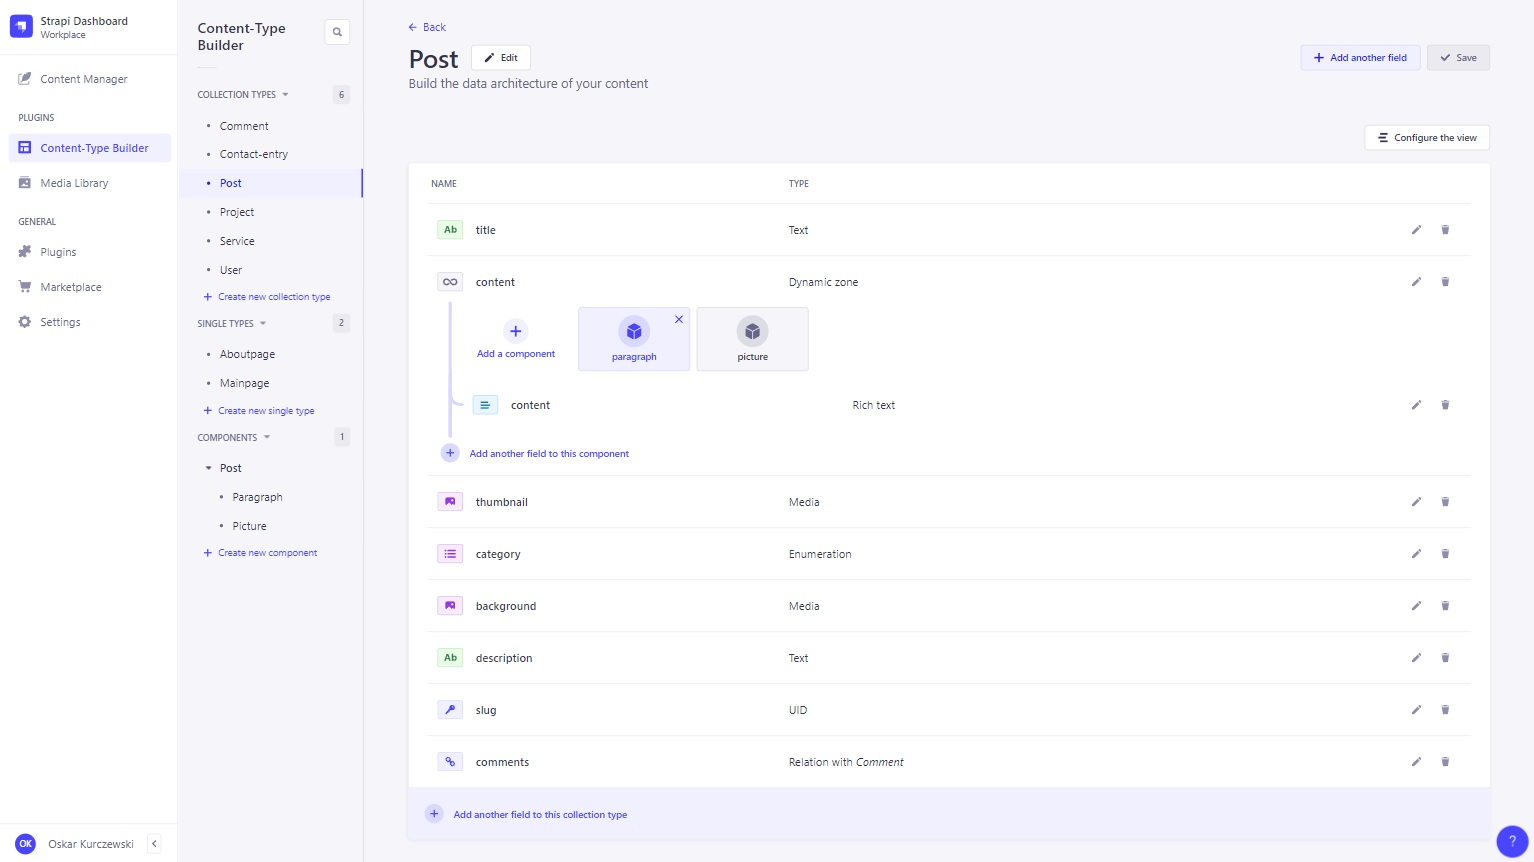
\includegraphics[width=0.95\textwidth]{images/strapi-interface-1.jpg}}
   \caption{Interfejs narzędzia Strapi z wtyczką Content-Type Builder.}
   \label{fig:strapi-interface-1.jpg}
\end{figure}

\begin{figure}[H] 
    \centering
         \fbox{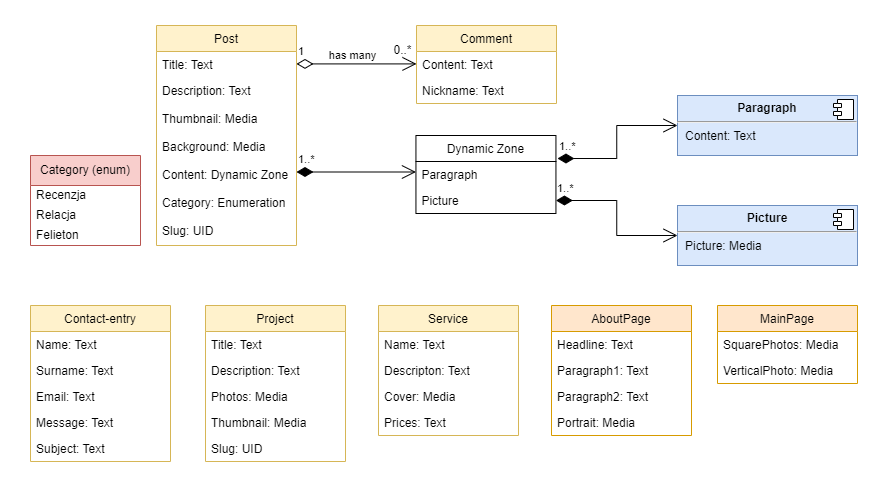
\includegraphics[width=0.95\textwidth]{images/diagram-typu-tresci.png}}
   \caption{Diagram struktury danych w systemie zarządzania treści Strapi.}
   \label{fig:diagram-typu-tresci.png}
\end{figure}

\newpage

Po zakończeniu tworzenia struktury danych konieczne jest ustawienie odpowiednich uprawnień dotyczących REST API w celu umożliwienia pobierania treści do wyświetlenia na stronie oraz zablokowania możliwości ich dodawania, usuwania i modyfikacji użytkownikom nieposiadającym konta w Strapi (reprezentowanych przez rolę \textit{Public}). Wyjątkami są komentarze, które mogą być dodawane pod postami przez każdą osobę odwiedzającą stronę oraz wpisy kontaktowe, które nie mogą być wyświetlane przez użytkowników, ale mogą być przez nich dodawane. Szczegółowa lista uprawnień dla roli \textit{Public} zaprezentowana jest w tabeli \ref{tab:permissions}. 

\begin{table}
    \centering
    \caption{Lista uprawnień do REST API w Strapi dla użytkownika z rolą \textit{Public} (niezalogowanego)}
    \begin{tabular}{|l|l|l|l|l|l|} 
        \hline
        \diagbox{\textbf{Element}}{\textbf{Uprawnienie}} & \textit{create} & \textit{delete} & \textit{update} & \textit{find} & \textit{findOne}  \\ 
        \hline
        Aboutpage                                        & n/d             &                 &                 & X             & n/d               \\ 
        \hline
        Mainpage                                         & n/d             &                 &                 & X             & n/d               \\ 
        \hline
        Comment                                          & X               &                 &                 & X             &                   \\ 
        \hline
        Contact-entry                                    & X               &                 &                 &               &                   \\ 
        \hline
        Post                                             &                 &                 &                 & X             & X                 \\ 
        \hline
        Project                                          &                 &                 &                 & X             & X                 \\ 
        \hline
        Service                                          &                 &                 &                 & X             & X                 \\
        \hline
        \end{tabular}
    \label{tab:permissions}
\end{table}

Aby po stronie widoku możliwe było utworzenie linków do postów oraz projektów w postaci unikalnego ciągu znaków, konieczne było wprowadzenie modyfikacji do kontrolera dla wspomnianych kolekcji, a dokładniej --- nadpisanie funkcji pobrania jednego elementu (\textit{findOne}). Aby to zrobić, należy podać klucz, według którego ma być szukany dany element: jest nim właśnie \textit{slug}. Aby dane były pobierane w~odpowiedni sposób trzeba ustawić parametr \textit{populate} dla zawartości elementu na wartość \textit{true}. Przykład modyfikacji kontrolera znajduje się w listingu~\ref{chapter4:controller}. 

Ostatnim (choć wpływającym jedynie na wygodę dodawania treści) krokiem jest skorzystanie z funkcjonalności Strapi pozwalającej na rozmieszczenie elementów w edytorze treści w taki sposób, który odpowiada układowi faktycznej strony (rys. \ref{fig:strapi-interface-3.jpg}). Dzięki temu można rozpocząć dodawanie treści w prosty i~intuicyjny sposób (rys. \ref{fig:strapi-interface-4.jpg}).

\begin{code}[htbp]
    \lstinputlisting{./code/controller.txt}
    \caption
    [Przykład modyfikacji do kontrolera REST API w systemie zarządzania treścią Strapi.]
    {Przykład modyfikacji do kontrolera REST API w systemie zarządzania treścią Strapi.}
    \label{chapter4:controller}
\end{code}

\begin{figure}[H] 
    \centering
         \fbox{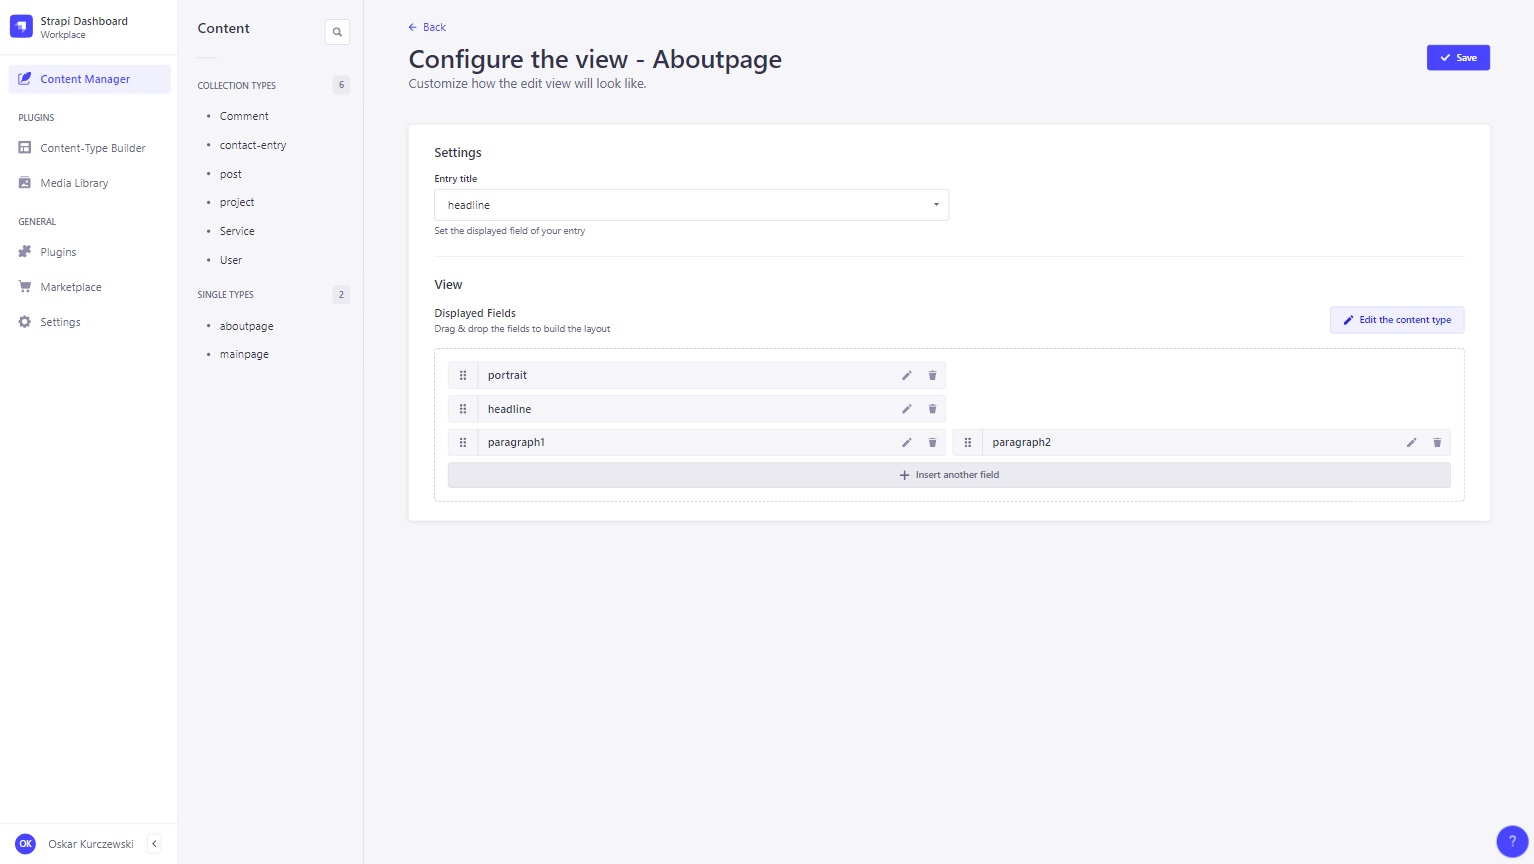
\includegraphics[width=0.95\textwidth]{images/strapi-interface-3.jpg}}
   \caption{Rozmieszczanie elementów edytora treści w systemie zarządzania treścią Strapi.}
   \label{fig:strapi-interface-3.jpg}
\end{figure}

\begin{figure}[H] 
    \centering
         \fbox{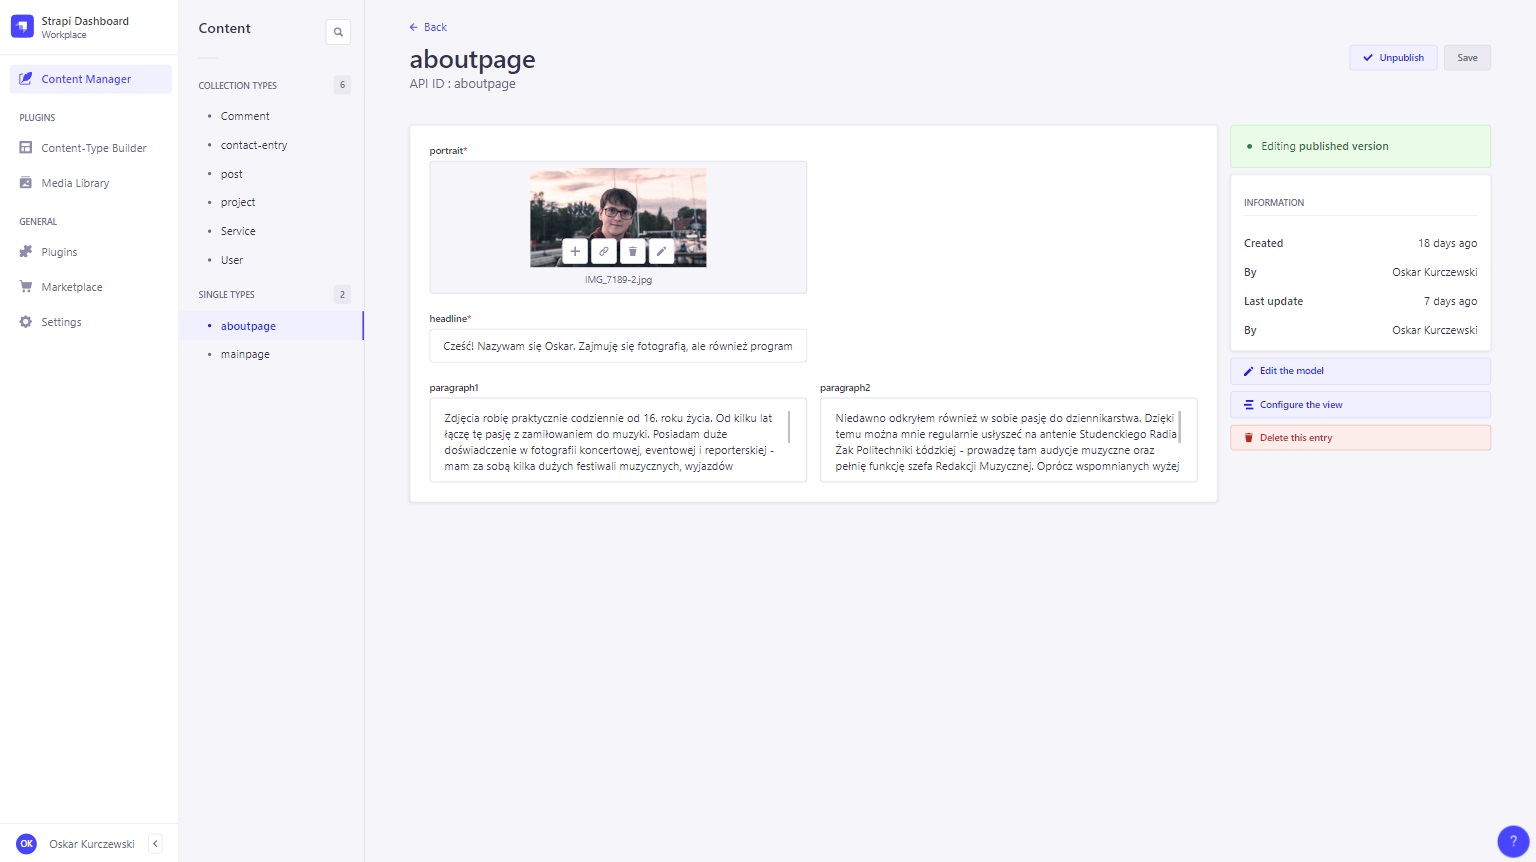
\includegraphics[width=0.95\textwidth]{images/strapi-interface-4.jpg}}
   \caption{Efekt rozmieszczenia elementów w edytorze treści w systemie zarządzania treścią Strapi.}
   \label{fig:strapi-interface-4.jpg}
\end{figure}

\subsubsection{Next.js --- implementacja strony internetowej}
Aby rozpocząć implementację aplikacji z wykorzystaniem Next.js, należy stworzyć i uruchomić nowy projekt z użyciem polecenia z listingu \ref{chapter4:npx_next.txt}. Konieczna jest też instalacja preprocesora Sass za pomocą menadżera pakietów npm. Po jej zakończeniu można rozpocząć pracę nad implementacją strony internetowej.

\begin{code}[htbp]
    \lstinputlisting{./code/npx_next.txt}
    \caption
    [Polecenie tworzące oraz uruchamiające nowy projekt z użyciem szkieletu aplikacyjnego Next.js.]
    {Polecenie tworzące oraz uruchamiające nowy projekt z użyciem szkieletu aplikacyjnego Next.js.}
    \label{chapter4:npx_next.txt}
\end{code}

\subsubsection*{Utworzenie projektu i organizacja jego struktury}
 Pierwszy krok to stworzenie plików odpowiadających odpowiednim podstronom w katalogu \texttt{/pages} --- szkielet aplikacyjny Next.js korzysta z routingu opartego na stronach będących komponentami biblioteki React \cite{nextdocs}. Potrzebne będą strona główna, strony portfolio i blogu (listy dodanych projektów/postów oraz widoki poszczególnych projektów/postów), strona z listą usług świadczonych przez fotografa, strona ``o~mnie'' oraz strona kontaktowa. Warto również dodać własną stronę ``nie znaleziono'', która jest wyświetlana, gdy dany link nie istnieje. Listing \ref{chapter4:tree} przedstawia drzewo plików w katalogu \texttt{/pages}. Warto w nim zwrócić uwagę na nawiasy kwadratowe przy plikach \texttt{blog/[slug].js} oraz \texttt{portfolio/[slug].js} --- oznacza to, że są to ścieżki dynamiczne, tzn. linki do postów oraz projektów generują się na podstawie parametru w postaci \textit{sluga} pobranego z systemu zarządzania treścią Strapi. 

\begin{code}[htbp]
    \lstinputlisting{./code/tree.txt}
    \caption
    [Drzewo plików w katalogu \texttt{/pages}.]
    {Drzewo plików w katalogu \texttt{/pages}.}
    \label{chapter4:tree}
\end{code}

\subsubsection*{Pobieranie danych z systemu zarządzania treścią}

Po utworzeniu odpowiedniej struktury plików w projekcie, można przejść do budowy układu poszczególnych stron oraz pobierania danych z systemu zarządzania treścią Strapi. Jako przykład posłuży strona ``o mnie'' znajdująca się w pliku \texttt{about.js}. Widoczny w listingu \ref{chapter4:next_about1.txt} komponent funkcyjny \textit{About} zwraca zawartość strony ``o~mnie'' w postaci kodu JSX. Funkcja \textit{getStaticProps} przedstawiona w listingu \ref{chapter4:next_about2.txt} służy natomiast do pobierania danych z systemu zarządzania treścią i statycznego generowania strony (SSG), dzięki czemu załaduje się ona szybciej oraz będzie lepiej indeksowana w wyszukiwarkach internetowych. W~przypadku danych, które po stronie systemu zarządzania treścią mogą być modyfikowane lub dodawane często, powinno się używać funkcji \textit{getServerSideProps}, oferującej renderowanie po stronie serwera (SSR). Różnica pomiędzy \textit{getStaticProps} a \textit{getServerSideProps} jest taka, że przy używaniu \textit{getStaticProps} zawartość strony zostanie wygenerowana w trakcie jej budowania, gdzie w przypadku \textit{getServerSideProps} renderowanie po stronie serwera ma miejsce za każdym razem, kiedy użytkownik wykona żądanie \cite{nextdocs}. Dzięki temu nie jest konieczne ponowne uruchomienie aplikacji Next.js w celu wyświetlenia nowo dodanych 
treści, co jest wymagane jeśli korzysta się z SSG. 

\begin{code}[htbp]
    \lstinputlisting{./code/next_about1.txt}
    \caption
    [Fragment pliku \texttt{about.js} przedstawiający komponent funkcyjny \textit{About}.]
    {Fragment pliku \texttt{about.js} przedstawiający komponent funkcyjny \textit{About}.}
    \label{chapter4:next_about1.txt}
\end{code}

\newpage

REST API systemu zarządzania treścią Strapi zwraca dane w formacie JSON (\textit{JavaScript Object Notation}). Listing \ref{chapter4:strapi_response.txt} przedstawia przykładowe, trywialne dane do strony ``o mnie''. Można je przekazać do komponentu \textit{About} w~formie właściwości (ang. \textit{props}), a następnie wyświetlić na stronie poprzez wskazanie konkretnego pola, czego przykładem jest linijka czternasta 
w listingu \ref{chapter4:next_about1.txt} odpowiadająca za wyświetlanie nagłówka.

\begin{code}[htbp]
    \lstinputlisting{./code/next_about2.txt}
    \caption
    [Fragment pliku \texttt{about.js} przedstawiający funkcję \textit{getStaticProps}.]
    {Fragment pliku \texttt{about.js} przedstawiający funkcję \textit{getStaticProps}.}
    \label{chapter4:next_about2.txt}
\end{code}

\begin{code}[htbp]
    \lstinputlisting{./code/strapi_response.txt}
    \caption
    [Dane w formacie JSON zwrócone przez Strapi dla strony ``o mnie''.]
    {Dane w formacie JSON zwrócone przez Strapi dla strony ``o mnie''.}
    \label{chapter4:strapi_response.txt}
\end{code}

\subsubsection*{Komponenty}

Aby zgodnie z zasadą pojedynczej odpowiedzialności \cite{srp} polepszyć czytelność kodu oraz ułatwić jego późniejszą ewentualną modyfikację, zostały stworzone następujące komponenty:
\begin{itemize}
    \item \textit{Card} --- znajdująca się na liście postów karta będąca jednocześnie odnośnikiem do strony z postem. Zawiera miniaturkę, kategorię, tytuł i~datę publikacji.
    \item \textit{Comment} --- komponent reprezentujący komentarz pod postem. Składa się z nazwy użytkownika, treści komentarza oraz czasu, który upłynął od jego publikacji (do jego obliczenia wykorzystana została prosta biblioteka \textit{react-time-ago} zainstalowana z użyciem menadżera pakietów npm).
    \item \textit{ImageModal} --- okno modalne zajmujące cały ekran, służące do wyświetlania zdjęcia z projektu w portfolio w dużym formacie.
    \item \textit{Service} --- komponent w formie karty zawierającej informacje na temat danej usługi (opis i cena), widoczne po najechaniu na obrazek, pod którym widnieje nazwa usługi.
    \item \textit{ProjectThumbnail} --- miniaturka projektu składająca się ze zdjęcia, opisu oraz przycisku ``więcej zdjęć'' przenoszącego do widoku całego projektu.
    \item \textit{Footer} --- stopka strony składająca się z informacji kontaktowych (telefon, adres poczty eletkronicznej) oraz odnośników do profilów fotografa w portalach społecznościowych.
    \item \textit{Navbar} --- pasek z nagłówkiem strony w postaci imienia i nazwiska fotografa oraz główne dziedziny świadczonych usług fotograficznych (w przypadku strony głównej) lub pasek nawigacyjny jeśli użytkownik znajduje się w innym miejscu.
\end{itemize}

\subsubsection*{Komentarze i formularz kontaktowy --- przesyłanie danych do Strapi}

Aby umożliwić dodawanie komentarzy pod postami oraz wysyłanie wiadomości poprzez formularz kontaktowy, należy w odpowiedni sposób przesłać dane do systemu zarządzania treścią Strapi z użyciem metody POST protokołu HTTP. Można to zrobić, używając funkcji \textit{fetch} z odpowiednimi parametrami tak, jak w~listingu \ref{chapter4:next_post.txt}. Owe parametry to \textit{method}, \textit{headers} oraz \textit{body}. \textit{Method} określa metodę HTTP (w tym przypadku POST), \textit{headers} to nagłówki HTTP do wysłania z żądaniem (tutaj: określające sposób przekazania danych), natomiast \textit{body} to przesyłane dane (w formacie JSON). Przy wysyłaniu żądania ważne jest również określenie jego adresu, którym w tym przypadku jest \texttt{/api/comments}. 

\begin{code}[htbp]
    \lstinputlisting{./code/next_post.txt}
    \caption
    [Fragment funkcji \textit{addComment} dodającej komentarz do postu.]
    {Fragment funkcji \textit{addComment} dodającej komentarz do postu.}
    \label{chapter4:next_post.txt}
\end{code}

\subsubsection*{Walidacja wprowadzanych danych}

Ze względu na to, że dane są przesyłane za pomocą formularza, należy sprawdzić poprawność wprowadzonych przez użytkownika danych za pomocą walidacji. W przypadku komentarza wystarczy atrybut \textit{required}, który blokuje możliwość wysłania danych jeśli pola treści oraz ksywki nie są wypełnione. Przy formularzu kontaktowym oprócz obowiązkowych pól, należy dodatkowo sprawdzić prawidłowość podawanego adresu poczty elektronicznej. Zostało to zrobione na dwa sposoby: w~samym formularzu z wykorzystaniem atrybutu ``\texttt{type="email"}'' oraz w~systemie zarządzania treścią Strapi poprzez zastosowanie wyrażenia regularnego.

\subsubsection*{\textit{Responsive Web Design}}

Jednym z wymagań niefunkcjonalnych projektu jest zastosowanie metody RWD (ang. \textit{Responsive Web Design}) w celu dostosowania tworzonej strony internetowej do ekranów różnych rozmiarów. Preprocesor Sass pozwala na zrobienie tego w bardzo prosty sposób, którym jest wykorzystanie zmiennych oraz domieszek (\textit{mixin}) --- fragmentów kodu SCSS pozwalających na używanie ich wielokrotnie bez konieczności ich kopiowania. Listing \ref{chapter4:mixin_example.txt} przedstawia deklarację zmiennej określającej szerokość ekranu średniej wielkości (np. tabletów) oraz domieszki pozwalającej ustawiać dla nich indywidualne zasady wyświetlania w sposób ukazany w~listingu~\ref{chapter4:include_example.txt}. 

\begin{code}[htbp]
    \lstinputlisting{./code/mixin_example.txt}
    \caption
    [Przykład deklaracji domieszki w SCSS.]
    {Przykład deklaracji domieszki w SCSS.}
    \label{chapter4:mixin_example.txt}
\end{code}

\begin{code}[htbp]
    \lstinputlisting{./code/include_example.txt}
    \caption
    [Przykład użycia domieszki w SCSS.]
    {Przykład użycia domieszki w SCSS.}
    \label{chapter4:include_example.txt}
\end{code}

% Portfolio i blog

\clearpage
\section{Portfolio i blog}

W tym rozdziale zaprezentowany zostanie efekt końcowy oraz sposób użytkowania stworzonej strony internetowej z perspektywy administratora (podrozdział \ref{strapi-use}) oraz użytkownika odwiedzającego stronę (podrozdział \ref{next-use}). Opisane będzie między innymi korzystanie z systemu zarządzania treścią (tworzenie, edycja i usuwanie zawartości strony, wyświetlanie wiadomości z formularza kontatkowego), dodawanie komentarzy i dostosowanie strony do ekranów różnej wielkości. 

%% System zarządzania treścią

\subsection{System zarządzania treścią} \label{strapi-use}

Jednym z dwóch głównych elementów tworzonej strony internetowej jest system zarządzania treścią, którym jest Strapi. Narzędzie to pozwala na intuicyjne dodawanie zawartości, która ma znaleźć się na stronie internetowej. Aby z niego skorzystać, należy zalogować się do panelu administracyjnego, gdzie dostępny jest menedżer treści (ang. \textit{Content Manager}) pozwalający na dodawanie, edycję i usuwanie treści, które są widoczne dla osób odwiedzających stronę. 

\subsubsection*{Wyświetlanie wiadomości wysłanych za pomocą formularza kontaktowego}

W celu wyświetlenia wiadomości wysłane za pomocą formularza kontaktowego należy przejść do kolekcji o nazwie \textit{contact-entry} w sekcji \textit{Content Manager} systemu zarządzania treścią Strapi. Znajduje się tam lista wpisów, które zostały dodane przez osoby odwiedzające stronę. Aby przeczytać konkretną wiadomość, należy wybrać ją z listy, która jest przedstawiona na rysunku \ref{fig:strapi-use-1.jpg}. 

\begin{figure}[H] 
    \centering
         \fbox{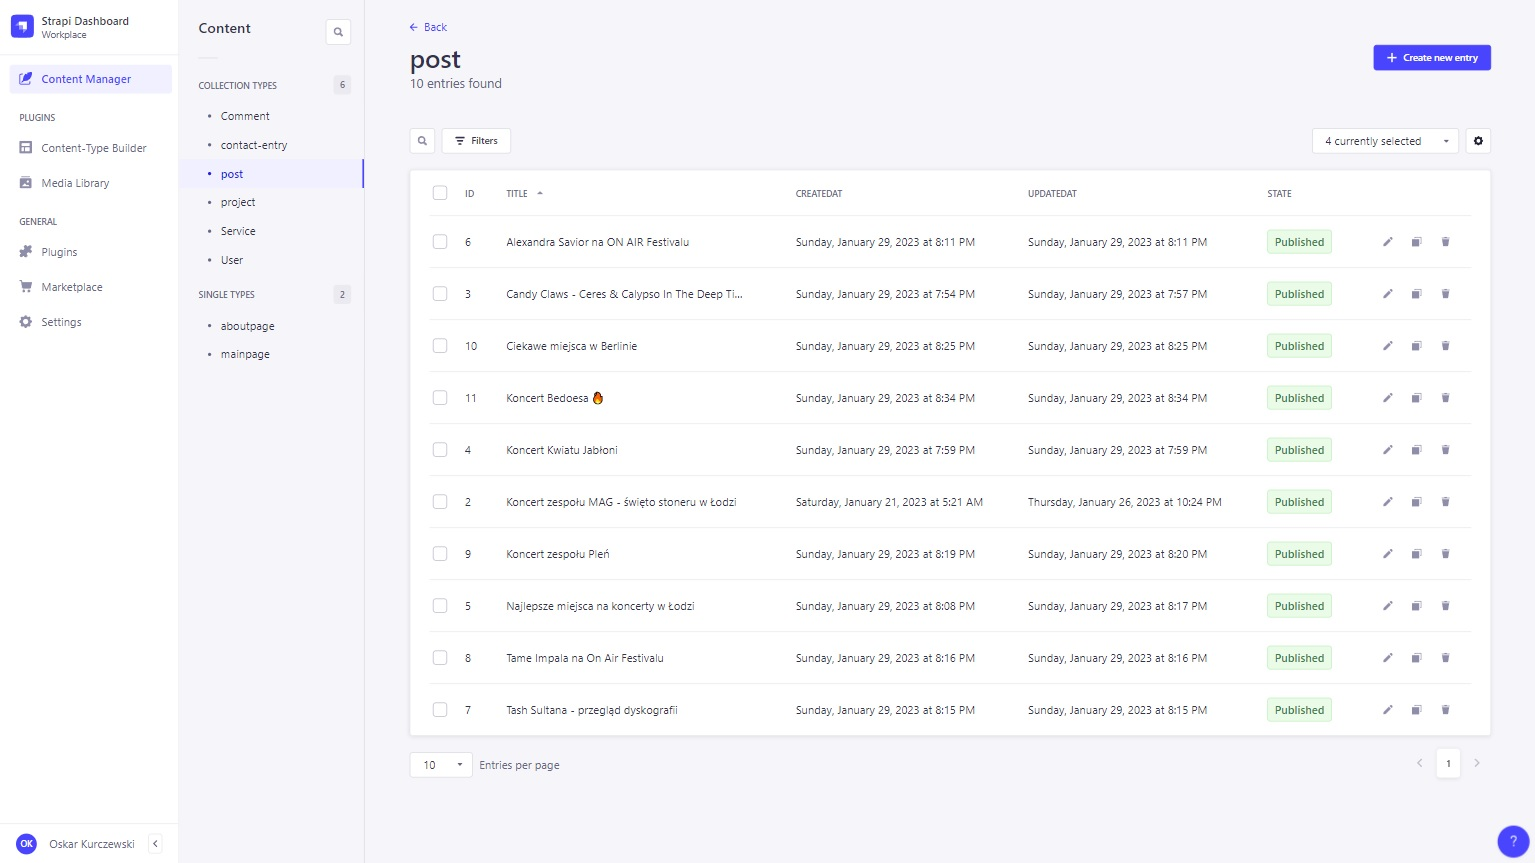
\includegraphics[width=0.95\textwidth]{images/strapi-use-1.jpg}}
   \caption{Widok menadżera treści w Strapi (lista wiadomości wysłanych z formularza kontaktowego).}
   \label{fig:strapi-use-1.jpg}
\end{figure}

\subsubsection*{Dodawanie, edycja i usuwanie treści}

Dodawanie, edycja i usuwanie treści w Strapi są bardzo prostymi czynnościami. Wszystko odbywa się za pomocą intuicyjnego graficznego interfejsu użytkownika. W tej sekcji jako przykład posłuży proces dodawania postu. Aby to zrobić, należy najpierw w menedżerze treści wybrać odpowiednią kolekcję, czyli \textit{post}. Wyświetli się wtedy lista podobna do tej z rysunku \ref{fig:strapi-use-1.jpg}, gdzie poprzez naciśnięcie przycisku ``\textit{Create an entry}'' należy otworzyć okno tworzenia nowej pozycji (rys. \ref{fig:strapi-use-2.jpg}). Kolejnym krokiem jest wypełnienie pól występujących w poście (rys. \ref{fig:strapi-use-3.jpg}). W przypadku dodawania obrazów i innych plików, należy je uprzednio przesłać do biblioteki multimediów (rys. \ref{fig:strapi-use-4.jpg}). Obrazy można też w prosty sposób przykadrować (rys. \ref{fig:strapi-use-5.jpg}). Edycja treści wygląda podobnie do jej dodawania, ale zamiast użycia przycisku ``\textit{Create an entry}'' należy wybrać z listy pozycję, która ma być zmieniona. Pozycje usuwa się za pomocą przycisku z ikoną kosza (akcję należy dodatkowo zatwierdzić). 

\begin{figure}[H] 
    \centering
         \fbox{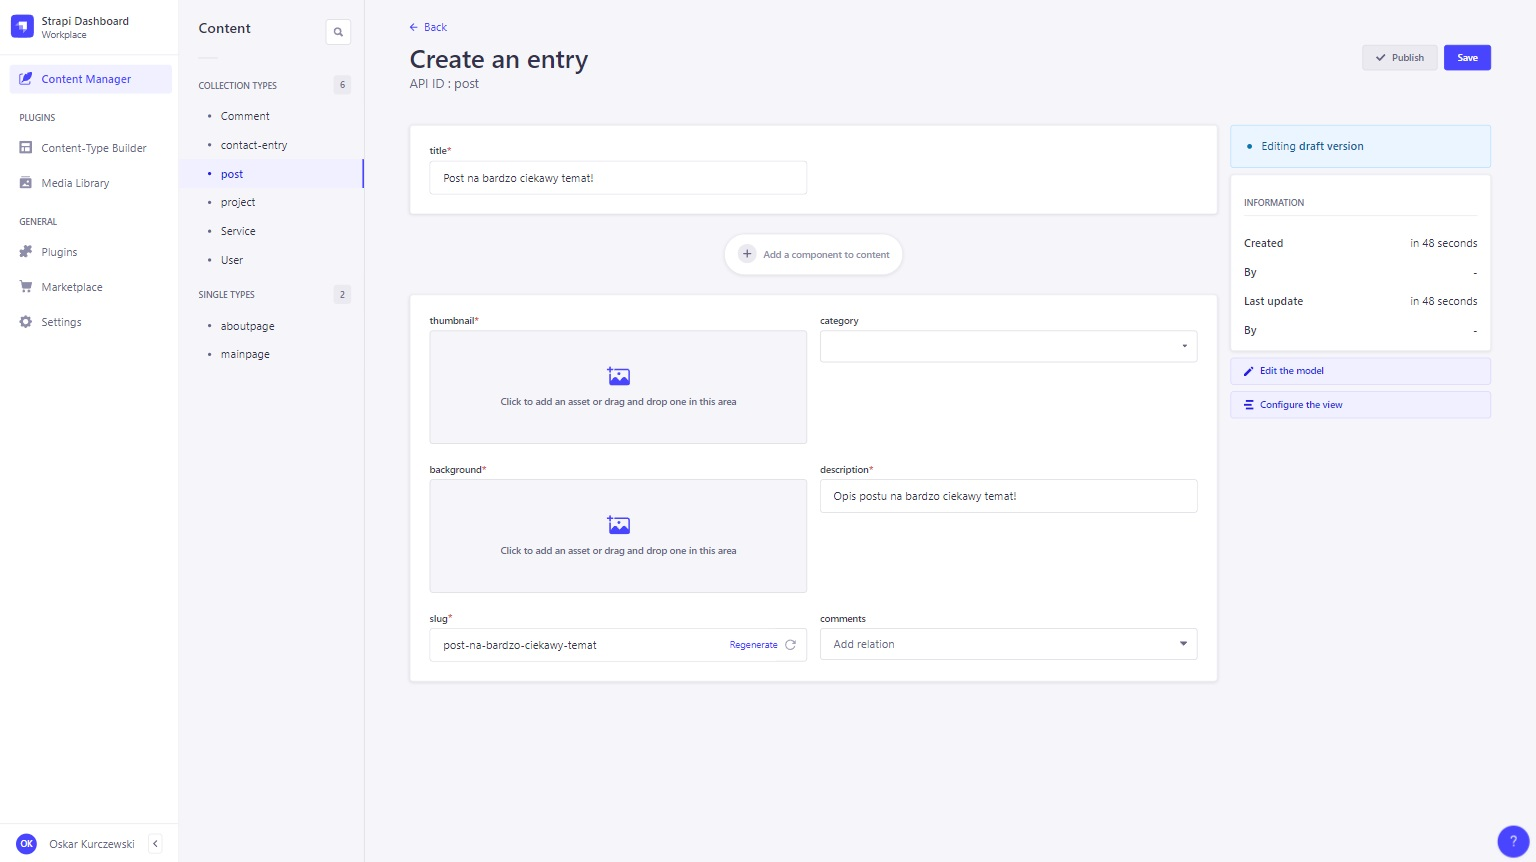
\includegraphics[width=0.95\textwidth]{images/strapi-use-2.jpg}}
   \caption{Widok menadżera treści w Strapi (tworzenie nowego postu --- pusty formularz).}
   \label{fig:strapi-use-2.jpg}
\end{figure}

\begin{figure}[H] 
    \centering
         \fbox{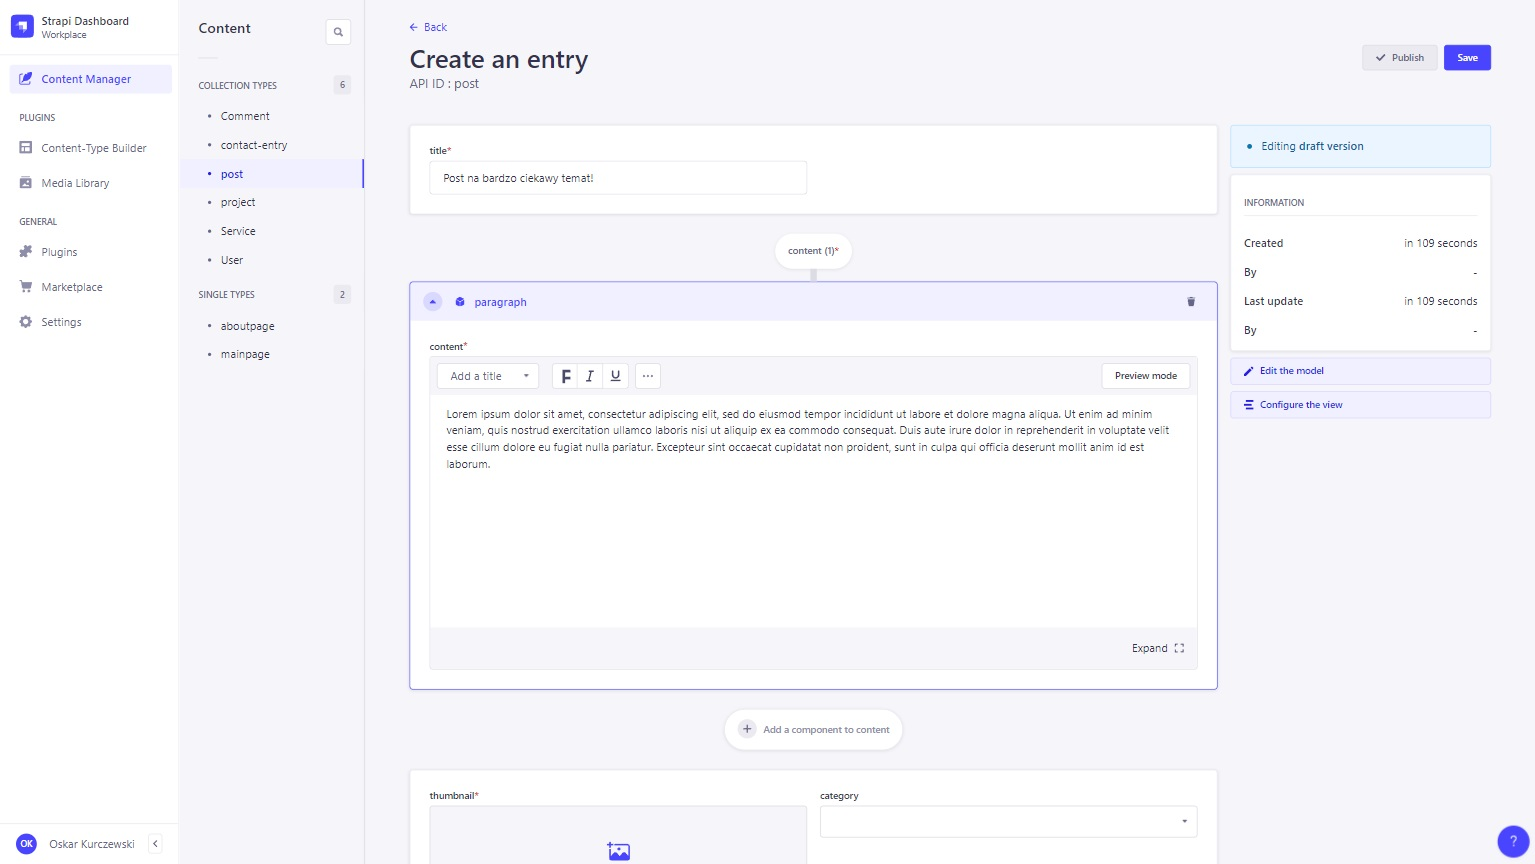
\includegraphics[width=0.95\textwidth]{images/strapi-use-3.jpg}}
   \caption{Widok menadżera treści w Strapi (tworzenie nowego postu --- dodawanie treści).}
   \label{fig:strapi-use-3.jpg}
\end{figure}

\begin{figure}[H] 
    \centering
         \fbox{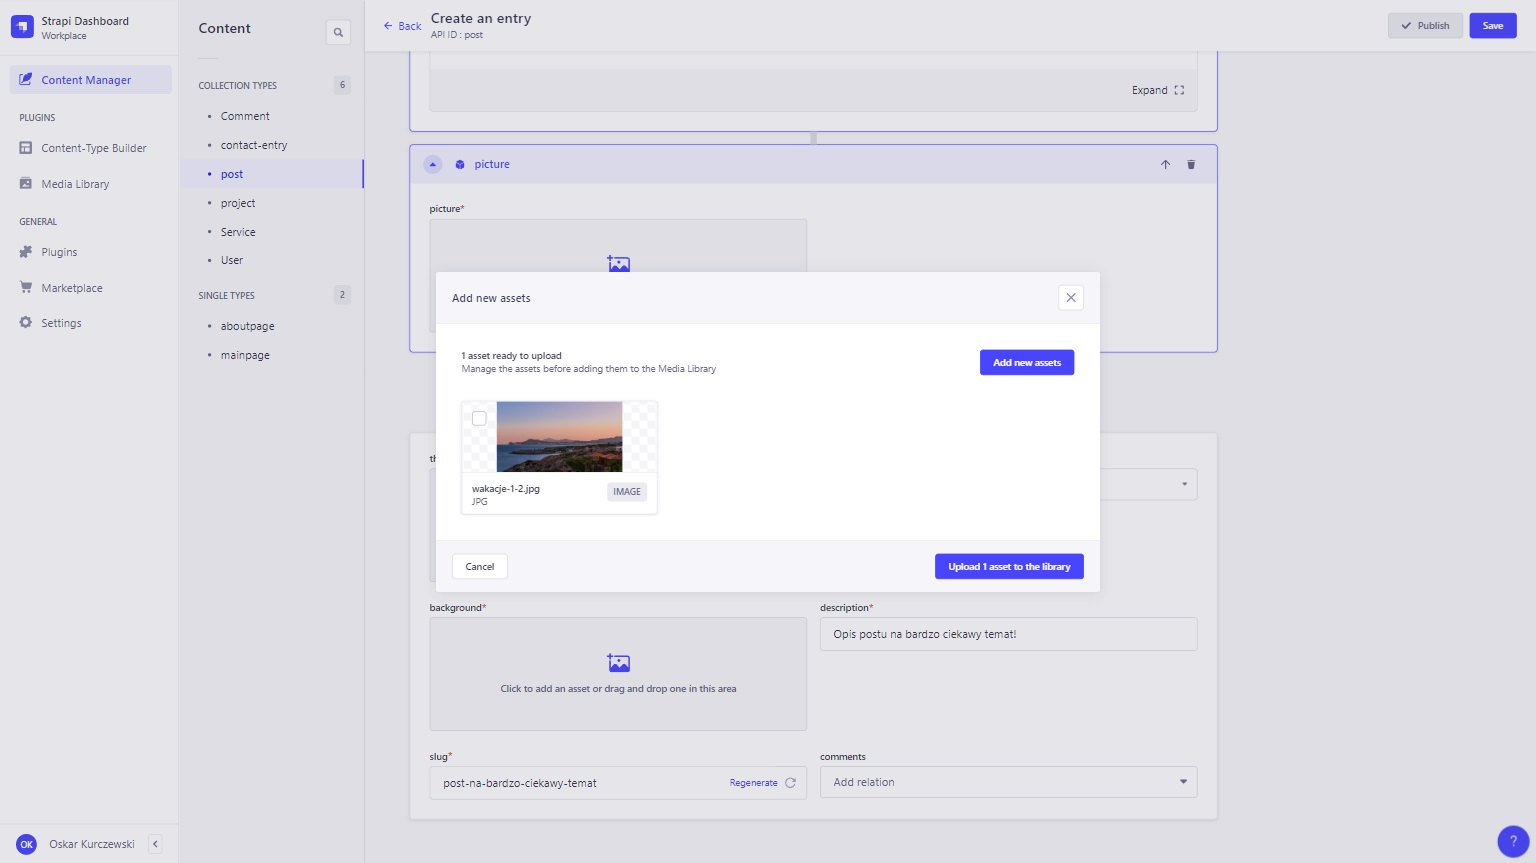
\includegraphics[width=0.95\textwidth]{images/strapi-use-4.jpg}}
   \caption{Widok menadżera treści w Strapi (tworzenie nowego postu --- przesyłanie nowego obrazu).}
   \label{fig:strapi-use-4.jpg}
\end{figure}

\begin{figure}[H] 
    \centering
         \fbox{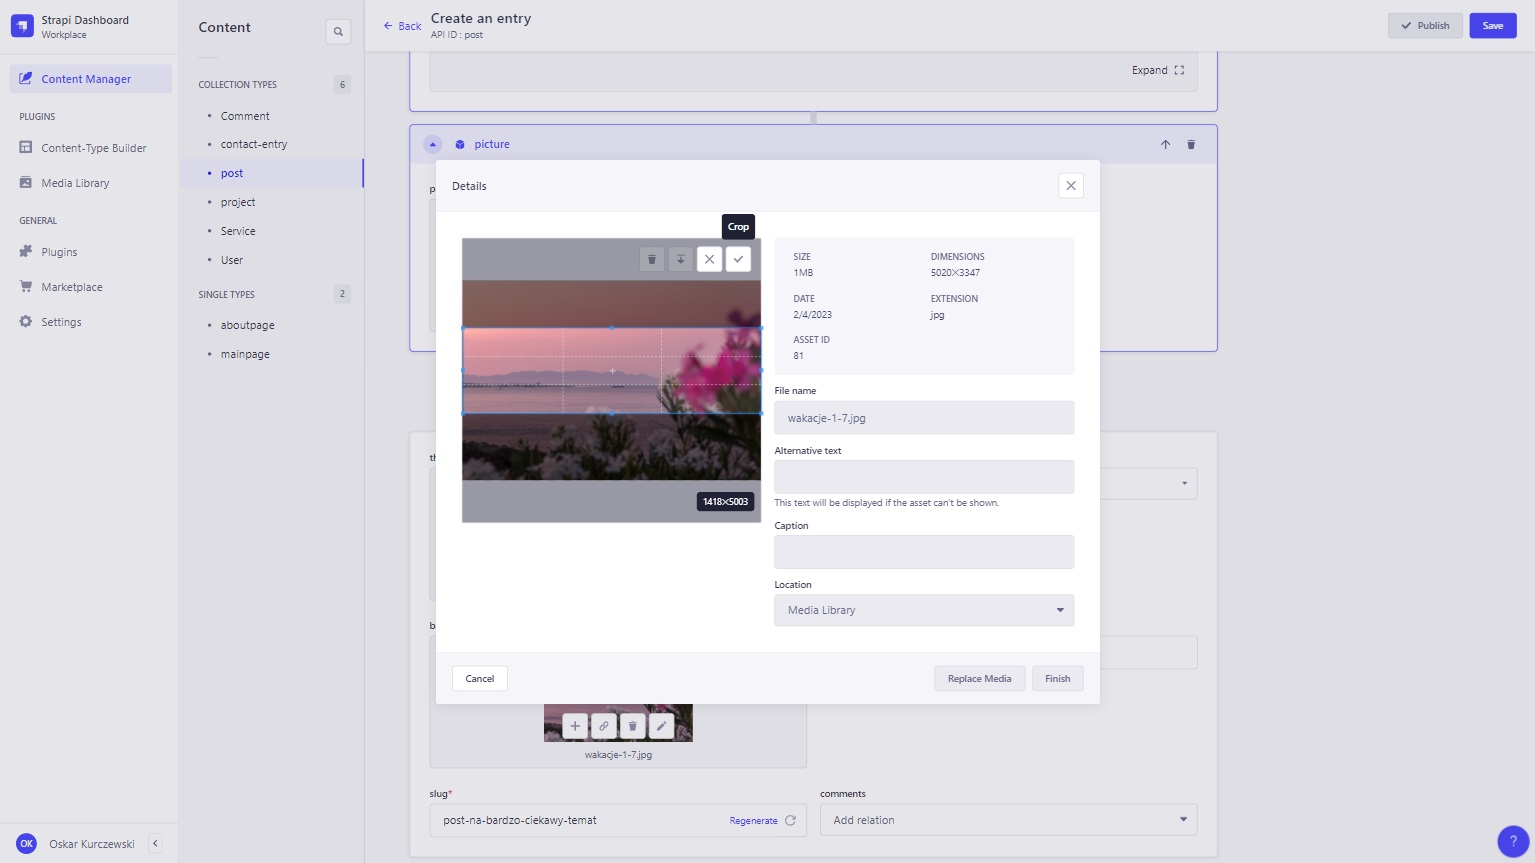
\includegraphics[width=0.95\textwidth]{images/strapi-use-5.jpg}}
   \caption{Widok menadżera treści w Strapi (przykład edycji obrazu).}
   \label{fig:strapi-use-5.jpg}
\end{figure}

%% Strona internetowa

\subsection{Strona internetowa} \label{next-use}

Strona internetowa z portfolio oraz blogiem jest drugą częścią stworzonego projektu i~odpowiada za prezentację treści zarządzanych z użyciem Strapi. W~tym podrozdziale przedstawione oraz opisane zostaną jej elementy oraz dopasowanie wyglądu strony do mniejszych ekranów (np. telefonów). 

\subsubsection*{Nagłówek i stopka}

Na stworzonej stronie internetowej pojawiły się dwa elementy, które są widoczne w każdej sekcji. Są to nagłówek strony pełniący głównie funkcję nawigacyjną i estetyczną oraz stopka, która umożliwia łatwy dostęp do najważniejszych informacji 
takich jak dane kontaktowe czy linki do mediów społecznościowych fotografa. 

\subsubsection*{Strona główna}

\begin{figure}[H] 
    \vspace{0.5cm}
    \centering
         \fbox{
\includegraphics[width=0.95\textwidth]{images/gotowa-aplikacja-1.jpg}}
   \caption{Widok strony głównej po najechaniu myszką na odnośnik do portfolio.}
   \label{fig:gotowa-aplikacja-1.jpg}
\end{figure}

Pierwszą rzeczą, którą widzą odwiedzający, jest strona główna (rys. \ref{fig:gotowa-aplikacja-1.jpg}). Składa się ona z trzech ułożonych w mozaikę zdjęć i menu, które jest połączeniem do pozostałych części strony --- portfolio, listy usług, blogu, strony ``o mnie'' i strony kontaktowej. Aby użytkownik wiedział, że jest to menu, zastosowano zanimowane podkreślenie tekstu i wskazującą strzałkę. Elementy te wyświetlają się po najechaniu na opcję myszką. 

\subsubsection*{Portfolio}

\begin{figure}[H] 
    \vspace{0.5cm}
    \centering
         \fbox{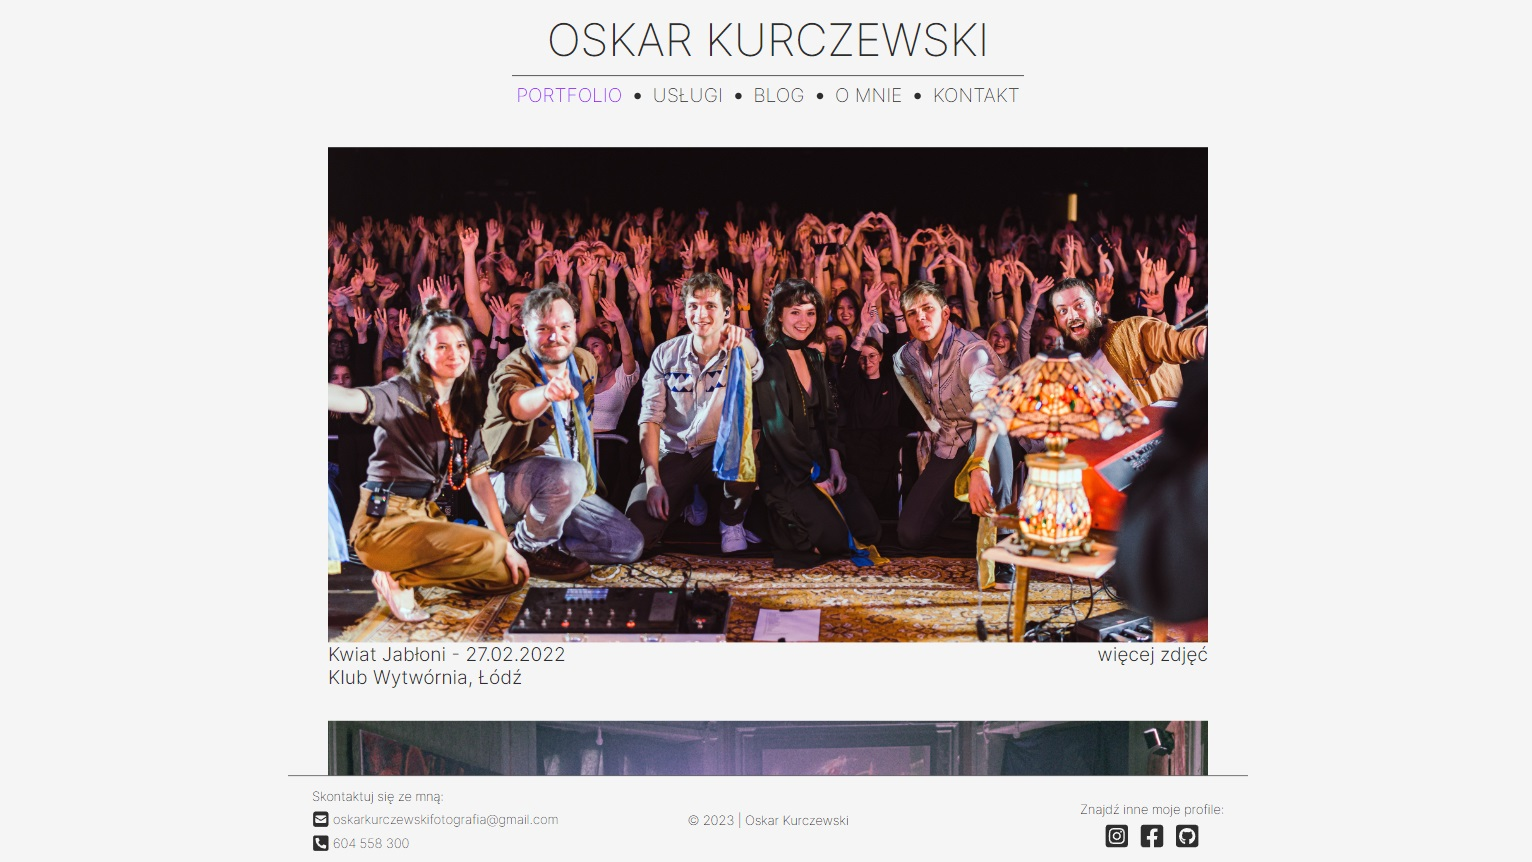
\includegraphics[width=0.95\textwidth]{images/gotowa-aplikacja-2.jpg}}
   \caption{Portfolio --- widok listy projektów.}
   \label{fig:gotowa-aplikacja-2.jpg}
\end{figure}

Jednym z najważniejszych elementów stworzonej strony internetowej jest portfolio służące do prezentacji zdjęć w formie tematycznych galerii (nazwanych projektami). Portfolio składa się z dwóch części. Pierwszą z nich jest lista projektów, widoczna na rysunku \ref{fig:gotowa-aplikacja-2.jpg} --- każdy projekt jest wyświetlany w formie zdjęcia oraz podpisu. Po naciśnięciu odnośnika ``więcej zdjęć'', użytkownik przenoszony jest do widoku wybranego projektu (rys. \ref{fig:gotowa-aplikacja-3.jpg}). Składa się on z nagłówka, podpisu oraz galerii zdjęć w formie dwukolumnowej mozaiki. Każdą fotografię można kliknąć w celu wyświetlenia jej w większym formacie (rys. \ref{fig:gotowa-aplikacja-4.jpg}). Aby zamknąć ten widok, wystarczy kliknąć przycisk ``zamknij''. 

\begin{figure}[H] 
    \centering
         \fbox{
\includegraphics[width=0.95\textwidth]{images/gotowa-aplikacja-3.jpg}}
   \caption{Portfolio --- widok projektu.}
   \label{fig:gotowa-aplikacja-3.jpg}
\end{figure}

\begin{figure}[H] 
    \centering
         \fbox{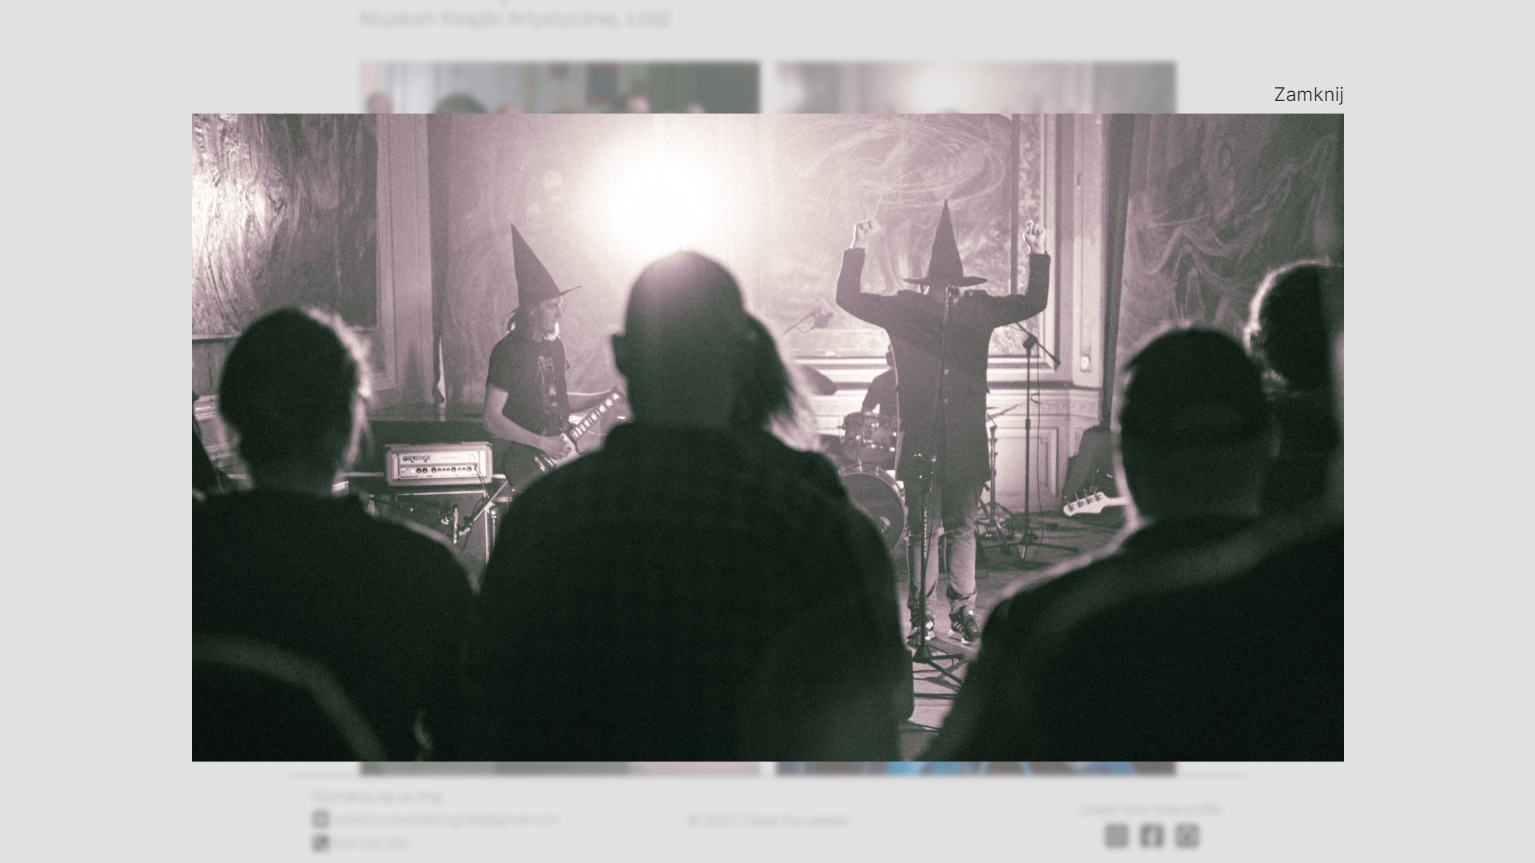
\includegraphics[width=0.95\textwidth]{images/gotowa-aplikacja-4.jpg}}
   \caption{Portfolio --- widok zdjęcia w większym formacie.}
   \vspace{-4mm}
   \label{fig:gotowa-aplikacja-4.jpg}
\end{figure}

\subsubsection*{Lista usług}

Sekcja zawierająca listę usług (rys. \ref{fig:gotowa-aplikacja-5.jpg}) jest natomiast jedną z najprostszych części całego projektu. Jej zadaniem jest przedstawienie charakterystyki świadczonych przez fotografa usług w formie krótkiego, chwytliwego opisu oraz informacji na temat ceny danej usługi. Wymienione dane pokazują się po najechaniu myszką na odpowiednią kartę --- obrazek wtedy zanika i widoczny jest tekst. 

\begin{figure}[H] 
    \centering
         \fbox{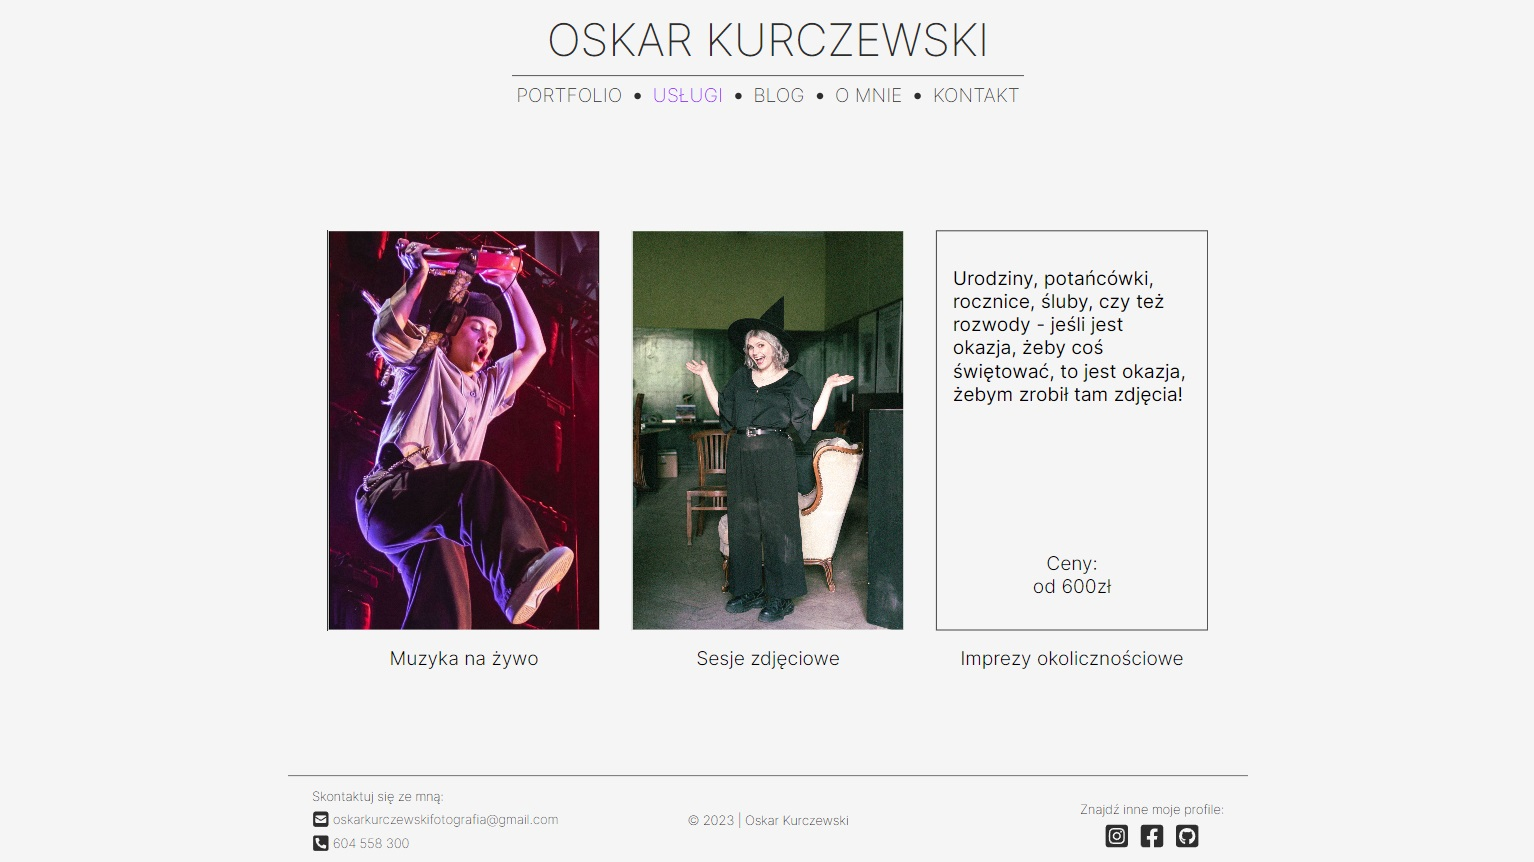
\includegraphics[width=0.95\textwidth]{images/gotowa-aplikacja-5.jpg}}
   \caption{Strona z listą usług po najechaniu na kartę z usługą ``imprezy okolicznościowe''.}
   \label{fig:gotowa-aplikacja-5.jpg}
\end{figure}

\subsubsection*{Blog i sekcja ``o mnie''}

Kolejną częścią stworzonej strony internetowej jest blog. Składa się on z widocznej na rysunku \ref{fig:gotowa-aplikacja-6.jpg} paginowanej listy postów reprezentowanych przez karty (na każdej stronie jest sześć takich kart). Pełnią one funkcję odnośników do poszczególnych postów. Widok postu (rys. \ref{fig:gotowa-aplikacja-7.jpg}) składa się z nagłówka zawierającego tytuł oraz opis na tle zdjęcia, pod którym znajduje się data dodania wpisu. Następnym elementem jest treść postu, która może składać się ze zdjęć (z podpisem lub bez) oraz tekstu. 

\begin{figure}[H] 
    \centering
         \fbox{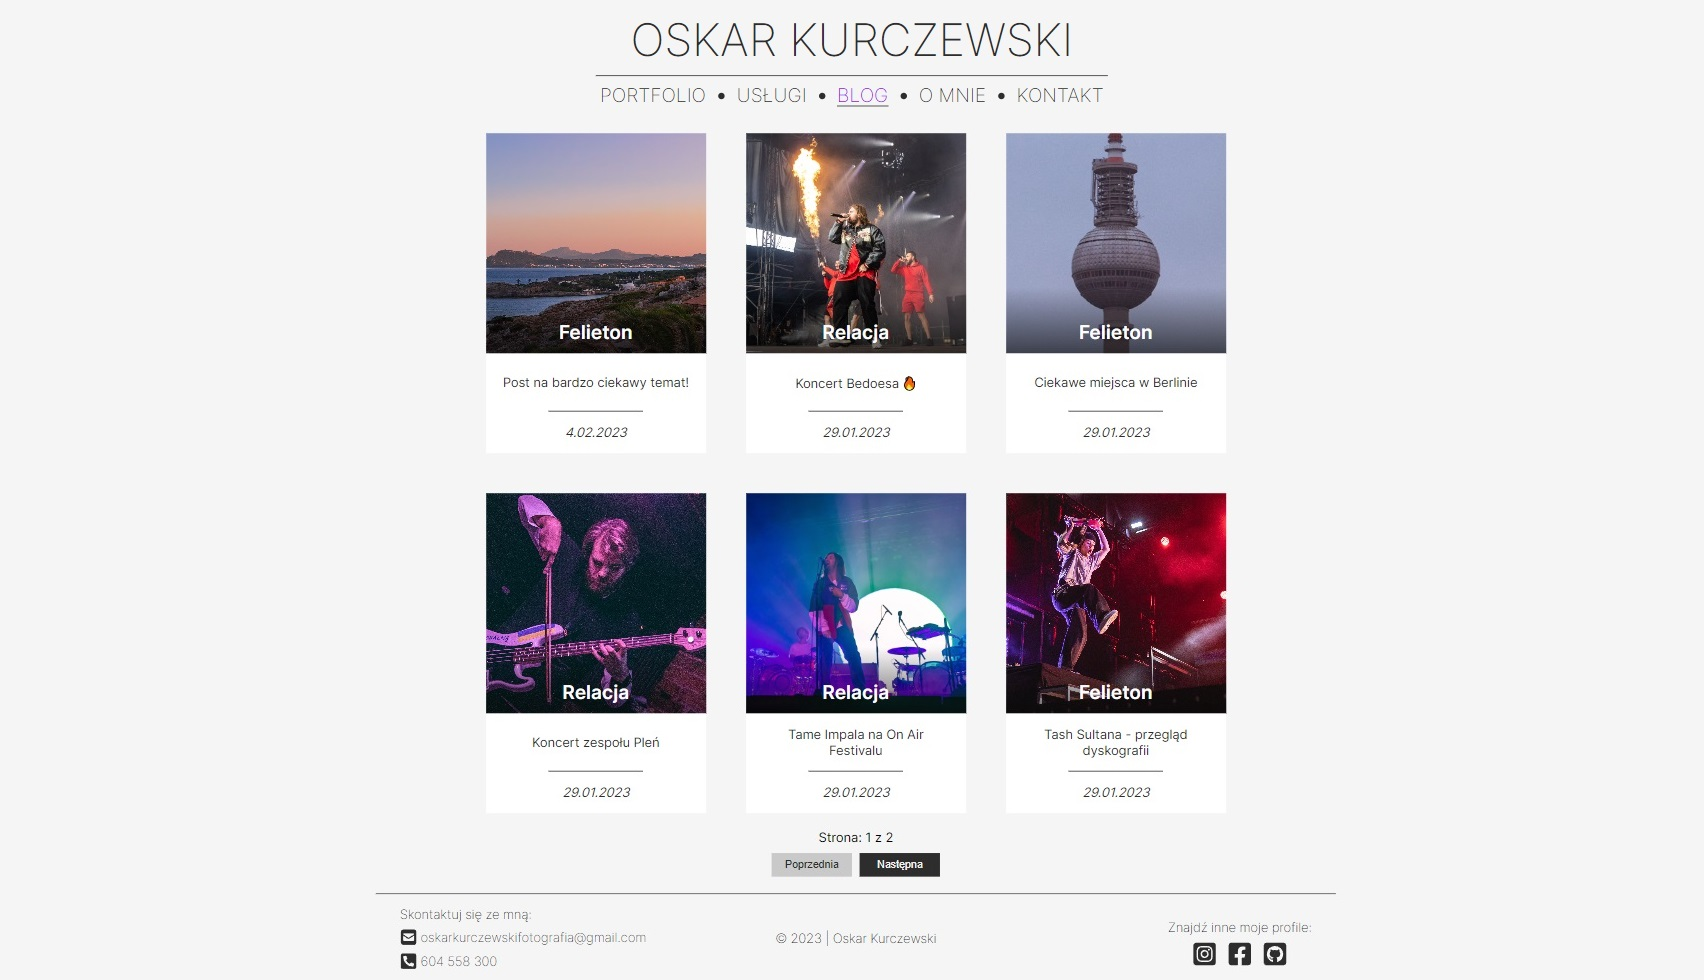
\includegraphics[width=0.95\textwidth]{images/gotowa-aplikacja-6.jpg}}
   \caption{Blog --- lista postów.}
   \label{fig:gotowa-aplikacja-6.jpg} 
\end{figure}

\begin{figure}[H] 
    \centering
         \fbox{
\includegraphics[width=0.95\textwidth]{images/gotowa-aplikacja-7.jpg}}
   \caption{Blog --- widok postu.}
   \label{fig:gotowa-aplikacja-7.jpg}
\end{figure}

Na końcu postu (rys. \ref{fig:gotowa-aplikacja-8.jpg}) znajduje się sekcja komentarzy. Najprostsza ze wszystkich sekcja ``o mnie'' (rys. \ref{fig:gotowa-aplikacja-9.jpg}) zawiera natomiast zdjęcie oraz opis zawierający informacje na temat osoby prezentującej swoje projekty na stronie. 

\begin{figure}[H] 
    \centering
         \fbox{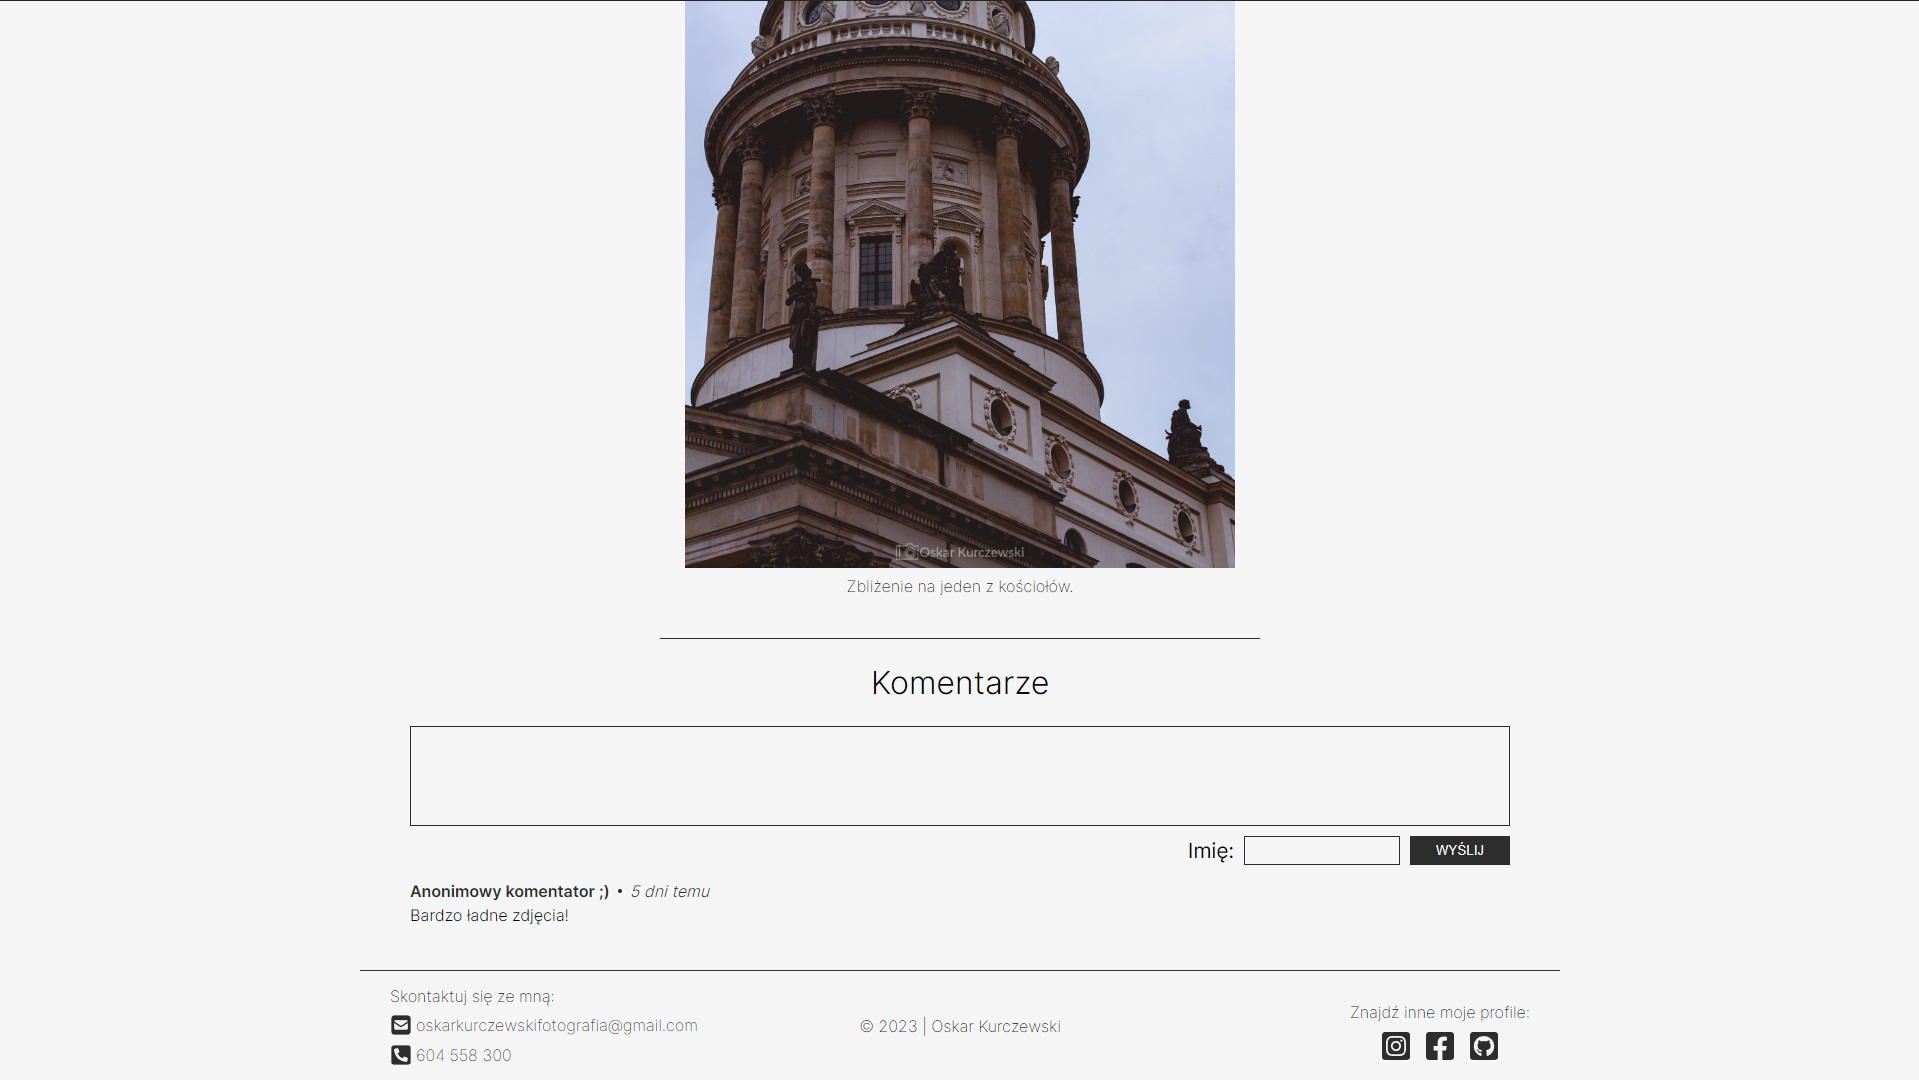
\includegraphics[width=0.95\textwidth]{images/gotowa-aplikacja-8.jpg}}
   \caption{Blog --- widok postu z komentarzem.}
   \vspace{-3mm}
   \label{fig:gotowa-aplikacja-8.jpg}
\end{figure}

\begin{figure}[H] 
    \centering
         \fbox{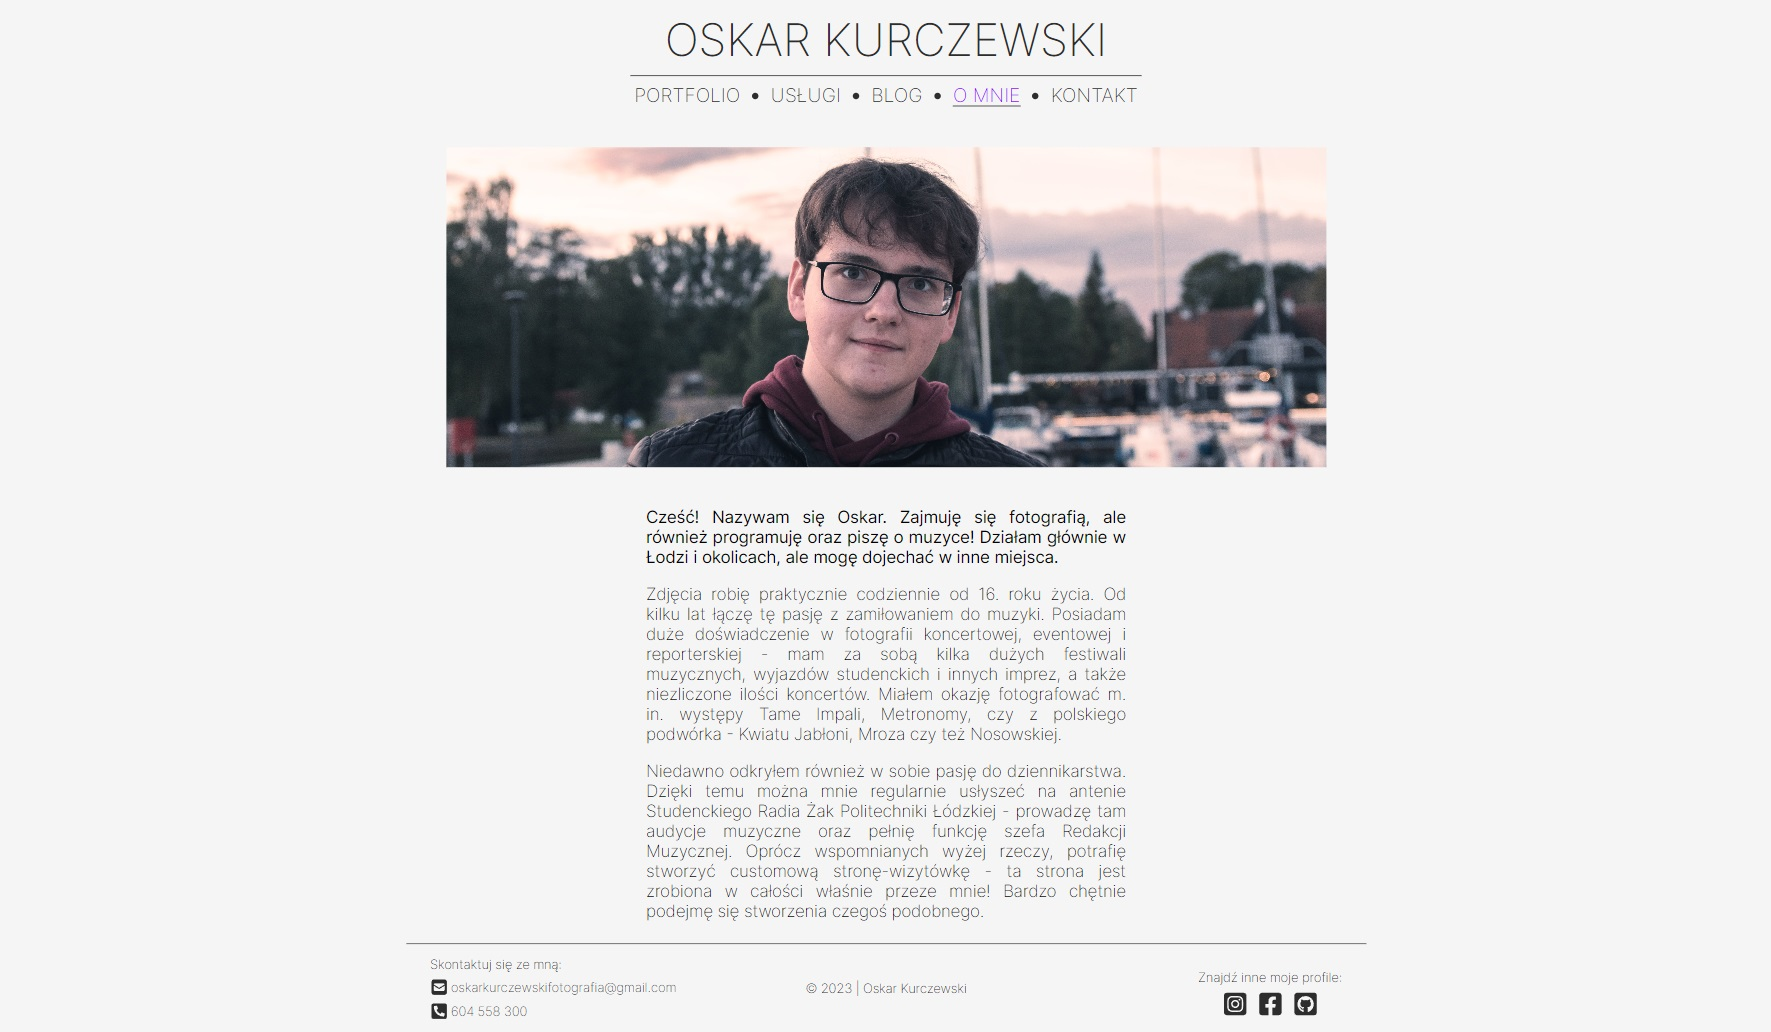
\includegraphics[width=0.95\textwidth]{images/gotowa-aplikacja-9.jpg}}
   \caption{Sekcja ``o mnie''.}
   \vspace{-3mm}
   \label{fig:gotowa-aplikacja-9.jpg}
\end{figure}

\subsubsection*{Strona kontaktowa}

\begin{figure}[H] 
    \centering
         \fbox{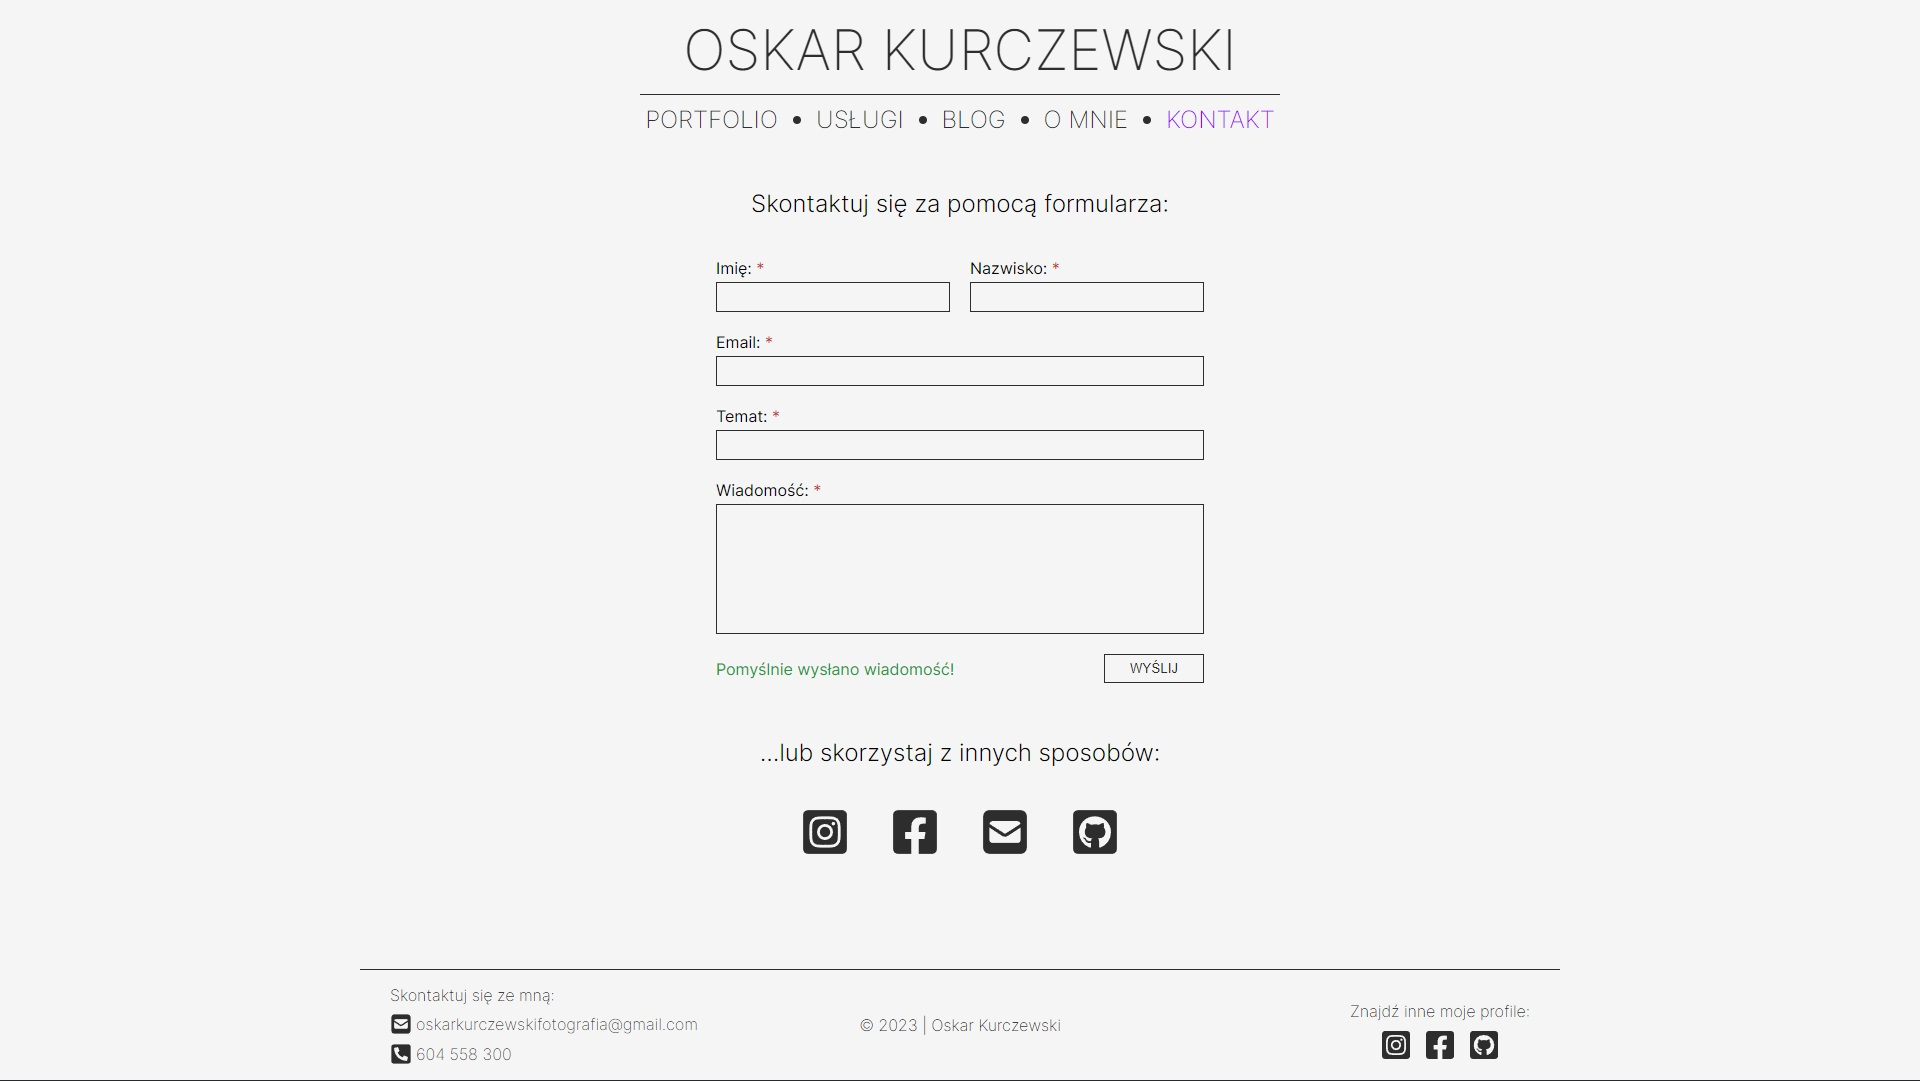
\includegraphics[width=0.95\textwidth]{images/gotowa-aplikacja-10.jpg}}
   \caption{Sekcja ``kontakt'' po poprawnym wysłaniu wiadomości z użyciem formularza.}
   \label{fig:gotowa-aplikacja-10.jpg}
\end{figure}

Ostatnia sekcja zawiera formularz kontaktowy i jest przedstawiona na rysunku \ref{fig:gotowa-aplikacja-10.jpg}. Umożliwia ona przesłanie wiadomości za pomocą formularza kontaktowego oraz zawiera odnośniki do mediów społecznościowych i adresu poczty elektronicznej. Rzeczą, na którą warto zwrócić uwagę jest, informacja o poprawnym wysłaniu wiadomości. Pozwala ona użytkownikowi upewnić się, że dotarła ona do systemu zarządzania treścią w poprawny sposób. 



\subsubsection*{Responsywność strony}

Strona internetowa z portfolio i blogiem została stworzona z zastosowaniem zasad RWD (\textit{Responsive Web Design}). Rysunek \ref{fig:resposywnosc.jpg} przedstawia widok strony głównej, projektu w portfolio oraz postu na blogu widziane na ekranie smartfona. 

\begin{figure}[H] 
    \centering
         \fbox{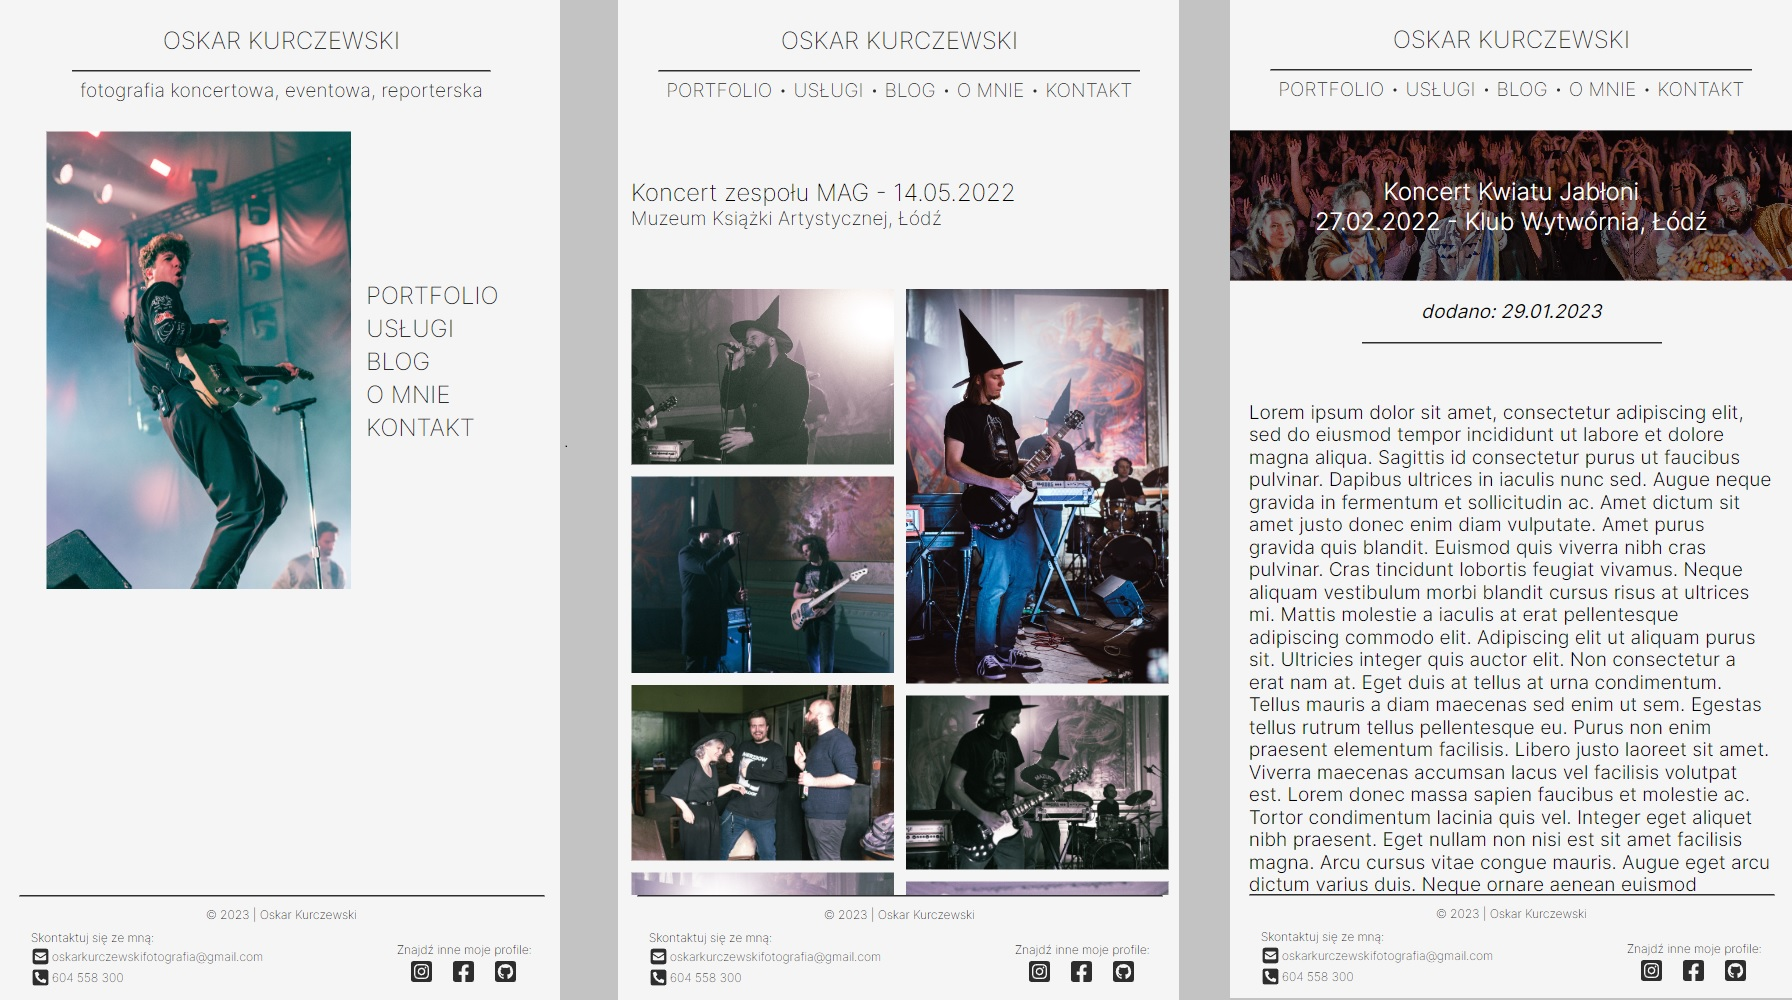
\includegraphics[width=0.95\textwidth]{images/resposywnosc.jpg}}
   \caption{Responsywność strony --- strona główna, projekt w portfolio oraz post na blogu.}
   \label{fig:resposywnosc.jpg}
\end{figure}

% Podsumowanie

\newpage 

\section{Podsumowanie}

% Spis rysunków

\newpage 

\addcontentsline{toc}{section}{\protect\numberline{}Spis rysunków}%
    \listoffigures
    \clearpage

% Spis tabel

\newpage 

\addcontentsline{toc}{section}{\protect\numberline{}Spis tabel}%
    \listoftables
    \clearpage

% Spis listingów

\newpage 

\addcontentsline{toc}{section}{\protect\numberline{}Spis listingów}%
    \listofcodes
    \clearpage

% Bibliografia

\newpage 

\section*{Bibliografia}
    \addcontentsline{toc}{section}{\protect\numberline{}Bibliografia}%
    \renewcommand{\section}[2]{}
    
\begin{thebibliography}{99}

    \bibitem{fotografia}
    Leszek J. Pękalski,
    \textit{Kalejdoskop fotografii. Między techniką a sztuką},
    Helion,
    2012.

    \bibitem{nobelfoto} 
    The Nobel Prize in Physics 2009,
    \url{https://www.nobelprize.org/prizes/physics/2009/summary/}, 
    dostęp 27.01.2023.

    \bibitem{firstdigitalphoto}
    The first digital photos, National Science and Media Museum,
    \url{https://www.scienceandmediamuseum.org.uk/objects-and-stories/first-digital-photos},
    dostęp 27.01.2023.

    \bibitem{instagram}
    Most followers on Instagram, Statista,
    \url{https://www.statista.com/statistics/421169/most-followers-instagram/},
    dostęp 27.01.2023.

    \bibitem{socialmediastats}
    Global social networks ranked by number of users, Statista,
    \url{https://www.statista.com/statistics/272014/global-social-networks-ranked-by-number-of-users/},
    dostęp 27.01.2023

    \bibitem{ashley}
    Ashley Osborn,
    \url{https://www.ashleyosborn.com/},
    dostęp 27.01.2023.

    \bibitem{stateofphotography}
    State of the Photography Industry Report 2022, Format,
    \url{https://www.format.com/magazine/features/photography/state-of-the-photography-industry-2022},
    dostęp 27.01.2023.

    \bibitem{projektowanie}
    Jason Beaird, James George,
    \textit{Niezawodne zasady web designu. Projektowanie spektakularnych witryn internetowych. Wydanie III},
    Helion,
    2015.

    \bibitem{formularze}
    Jennifer Niederst Robbins,
    \textit{Projektowanie stron internetowych. Przewodnik dla początkujących webmasterów po HTML5, CSS3 i grafice. Wydanie IV},
    Helion,
    2014.

    \bibitem{szerokosc}
    Line Length Readability, Baymard,
    \url{https://baymard.com/blog/line-length-readability},
    dostęp 27.01.2023

    \bibitem{socialmedia}
    Marcin Żukowski,
    \textit{Twoja firma w social mediach. Podręcznik marketingu internetowego dla małych i średnich przedsiębiorstw},
    Helion,
    2016.

    \bibitem{figma}
    Fabio Staiano,
    \textit{Designing and Prototyping Interfaces with Figma},
    Packt Publishing,
    2022.

    \bibitem{js}
    David Flanagan,
    \textit{JavaScript. Przewodnik. Poznaj język mistrzów programowania. Wydanie VII},
    Helion,
    2021.

    \bibitem{historiafacebooka}
    Facebook Overview, History \& Facts, Britannica,
    \textit{https://www.britannica.com/topic/Facebook},
    dostęp 27.01.2023.

    \bibitem{stories}
    Introducing Instagram Stories,
    \textit{https://about.instagram.com/blog/announcements/introducing-instagram-stories},
    dostęp 27.01.2023.

    \bibitem{instagramfirstday}
    A Brief History of Instagram's Fateful First Day, Time,
    \textit{https://time.com/4408374/instagram-anniversary/},
    dostęp 27.01.2023.

    \bibitem{strapidocs}
    Strapi Developer Docs,
    \textit{https://docs.strapi.io/developer-docs/latest/getting-started/introduction.html},
    dostęp 27.01.2023.

    \bibitem{strapifeatures}
    Strapi Features,
    \textit{https://strapi.io/features},
    dostęp 27.01.2023.

    \bibitem{node}
    About Node.js,
    \textit{https://nodejs.org/en/about/},
    dostęp 27.01.2023.

    \bibitem{npm}
    About npm,
    \textit{https://www.npmjs.com/about},
    dostęp 27.01.2023.

    \bibitem{sqlite}
    About SQLite,
    \textit{https://www.sqlite.org/about.html},
    dostęp 27.01.2023.

    \bibitem{react}
    React - A JavaScript library for building user interfaces,
    {https://reactjs.org},
    dostęp 27.01.2023.

    \bibitem{next}
    Next.js by Vercel - the React framework,
    {https://nextjs.org},
    dostęp 27.01.2023. 

    \bibitem{nextdocs}
    Next.js Documentation,
    {https://nextjs.org/docs/getting-started},
    dostęp 27.01.2023.

    \bibitem{sass}
    Sass basics,
    {https://sass-lang.com/guide},
    dostęp 27.01.2023.

    \bibitem{wymagania}
    Karl E Wiegers, Joy Beatty,
    \textit{Specyfikacja oprogramowania. Inżynieria wymagań. Wydanie III},
    Helion,
    2014.
    
    \bibitem{seo}
    Eric Enge, Stephan Spencer, Jessie Stricchiola,
    \textit{SEO, czyli sztuka optymalizacji witryn dla wyszukiwarek},
    Helion,
    2016.

    \bibitem{rwd}
    Thoriq Firdaus,
    \textit{Responsive Web Design. Nowoczesne strony WWW na przykładach},
    Helion, 
    2014.

    \bibitem{srp}
    Gary McLean Hall,
    \textit{Adaptywny kod. Zwinne programowanie, wzorce projektowe i SOLID-ne zasady. Wydanie II},
    Helion,
    2017.

        
\end{thebibliography}

\end{sloppypar}
\end{document}